\documentclass[twoside]{book}

% Packages required by doxygen
\usepackage{fixltx2e}
\usepackage{calc}
\usepackage{doxygen}
\usepackage[export]{adjustbox} % also loads graphicx
\usepackage{graphicx}
\usepackage[utf8]{inputenc}
\usepackage{makeidx}
\usepackage{multicol}
\usepackage{multirow}
\PassOptionsToPackage{warn}{textcomp}
\usepackage{textcomp}
\usepackage[nointegrals]{wasysym}
\usepackage[table]{xcolor}

% Font selection
\usepackage[T1]{fontenc}
\usepackage[scaled=.90]{helvet}
\usepackage{courier}
\usepackage{amssymb}
\usepackage{sectsty}
\renewcommand{\familydefault}{\sfdefault}
\allsectionsfont{%
  \fontseries{bc}\selectfont%
  \color{darkgray}%
}
\renewcommand{\DoxyLabelFont}{%
  \fontseries{bc}\selectfont%
  \color{darkgray}%
}
\newcommand{\+}{\discretionary{\mbox{\scriptsize$\hookleftarrow$}}{}{}}

% Page & text layout
\usepackage{geometry}
\geometry{%
  a4paper,%
  top=2.5cm,%
  bottom=2.5cm,%
  left=2.5cm,%
  right=2.5cm%
}
\tolerance=750
\hfuzz=15pt
\hbadness=750
\setlength{\emergencystretch}{15pt}
\setlength{\parindent}{0cm}
\setlength{\parskip}{3ex plus 2ex minus 2ex}
\makeatletter
\renewcommand{\paragraph}{%
  \@startsection{paragraph}{4}{0ex}{-1.0ex}{1.0ex}{%
    \normalfont\normalsize\bfseries\SS@parafont%
  }%
}
\renewcommand{\subparagraph}{%
  \@startsection{subparagraph}{5}{0ex}{-1.0ex}{1.0ex}{%
    \normalfont\normalsize\bfseries\SS@subparafont%
  }%
}
\makeatother

% Headers & footers
\usepackage{fancyhdr}
\pagestyle{fancyplain}
\fancyhead[LE]{\fancyplain{}{\bfseries\thepage}}
\fancyhead[CE]{\fancyplain{}{}}
\fancyhead[RE]{\fancyplain{}{\bfseries\leftmark}}
\fancyhead[LO]{\fancyplain{}{\bfseries\rightmark}}
\fancyhead[CO]{\fancyplain{}{}}
\fancyhead[RO]{\fancyplain{}{\bfseries\thepage}}
\fancyfoot[LE]{\fancyplain{}{}}
\fancyfoot[CE]{\fancyplain{}{}}
\fancyfoot[RE]{\fancyplain{}{\bfseries\scriptsize Generated by Doxygen }}
\fancyfoot[LO]{\fancyplain{}{\bfseries\scriptsize Generated by Doxygen }}
\fancyfoot[CO]{\fancyplain{}{}}
\fancyfoot[RO]{\fancyplain{}{}}
\renewcommand{\footrulewidth}{0.4pt}
\renewcommand{\chaptermark}[1]{%
  \markboth{#1}{}%
}
\renewcommand{\sectionmark}[1]{%
  \markright{\thesection\ #1}%
}

% Indices & bibliography
\usepackage{natbib}
\usepackage[titles]{tocloft}
\setcounter{tocdepth}{3}
\setcounter{secnumdepth}{5}
\makeindex

% Hyperlinks (required, but should be loaded last)
\usepackage{ifpdf}
\ifpdf
  \usepackage[pdftex,pagebackref=true]{hyperref}
\else
  \usepackage[ps2pdf,pagebackref=true]{hyperref}
\fi
\hypersetup{%
  colorlinks=true,%
  linkcolor=blue,%
  citecolor=blue,%
  unicode%
}

% Custom commands
\newcommand{\clearemptydoublepage}{%
  \newpage{\pagestyle{empty}\cleardoublepage}%
}

\usepackage{caption}
\captionsetup{labelsep=space,justification=centering,font={bf},singlelinecheck=off,skip=4pt,position=top}

%===== C O N T E N T S =====

\begin{document}

% Titlepage & ToC
\hypersetup{pageanchor=false,
             bookmarksnumbered=true,
             pdfencoding=unicode
            }
\pagenumbering{roman}
\begin{titlepage}
\vspace*{7cm}
\begin{center}%
{\Large Lattice\+Yang\+Mills }\\
\vspace*{1cm}
{\large Generated by Doxygen 1.8.11}\\
\end{center}
\end{titlepage}
\clearemptydoublepage
\tableofcontents
\clearemptydoublepage
\pagenumbering{arabic}
\hypersetup{pageanchor=true}

%--- Begin generated contents ---
\chapter{Lattice\+Yang\+Mills}
\label{index}\hypertarget{index}{}Suite for generating field configurations in pure YM S\+U(3) theory and compute basic observables on them. 
\chapter{Hierarchical Index}
\section{Class Hierarchy}
This inheritance list is sorted roughly, but not completely, alphabetically\+:\begin{DoxyCompactList}
\item \contentsline{section}{Action}{\pageref{classAction}}{}
\begin{DoxyCompactList}
\item \contentsline{section}{Pure\+Gauge}{\pageref{classPureGauge}}{}
\end{DoxyCompactList}
\item addable\begin{DoxyCompactList}
\item \contentsline{section}{S\+U3}{\pageref{structSU3}}{}
\end{DoxyCompactList}
\item addable\+\_\+left\begin{DoxyCompactList}
\item \contentsline{section}{S\+U3}{\pageref{structSU3}}{}
\end{DoxyCompactList}
\item \contentsline{section}{App}{\pageref{classApp}}{}
\begin{DoxyCompactList}
\item \contentsline{section}{Gauge\+Field\+Factory}{\pageref{classGaugeFieldFactory}}{}
\item \contentsline{section}{Gauge\+Field\+Reader}{\pageref{classGaugeFieldReader}}{}
\item \contentsline{section}{Wilson\+Flow}{\pageref{classWilsonFlow}}{}
\end{DoxyCompactList}
\item commutative\+\_\+addable\begin{DoxyCompactList}
\item \contentsline{section}{S\+U3}{\pageref{structSU3}}{}
\end{DoxyCompactList}
\item \contentsline{section}{complex}{\pageref{structcomplex}}{}
\item \contentsline{section}{Field$<$ T, N $>$}{\pageref{classField}}{}
\item \contentsline{section}{Lattice\+IO\+:\+:Input\+Conf}{\pageref{classLatticeIO_1_1InputConf}}{}
\item \contentsline{section}{Lattice$<$ T $>$}{\pageref{classLattice}}{}
\item \contentsline{section}{Lattice$<$ S\+U3 $>$}{\pageref{classLattice}}{}
\item \contentsline{section}{Lattice\+Units}{\pageref{structLatticeUnits}}{}
\item multipliable\begin{DoxyCompactList}
\item \contentsline{section}{S\+U3}{\pageref{structSU3}}{}
\item \contentsline{section}{S\+U3}{\pageref{structSU3}}{}
\end{DoxyCompactList}
\item \contentsline{section}{Observable}{\pageref{classObservable}}{}
\begin{DoxyCompactList}
\item \contentsline{section}{Energy\+Density}{\pageref{classEnergyDensity}}{}
\item \contentsline{section}{Plaquette}{\pageref{classPlaquette}}{}
\item \contentsline{section}{Super\+Obs}{\pageref{classSuperObs}}{}
\item \contentsline{section}{Topological\+Charge}{\pageref{classTopologicalCharge}}{}
\end{DoxyCompactList}
\item \contentsline{section}{Lattice\+IO\+:\+:Output\+Conf}{\pageref{classLatticeIO_1_1OutputConf}}{}
\item \contentsline{section}{Lattice\+IO\+:\+:Output\+Obs}{\pageref{classLatticeIO_1_1OutputObs}}{}
\item \contentsline{section}{Lattice\+IO\+:\+:Output\+Term}{\pageref{classLatticeIO_1_1OutputTerm}}{}
\item \contentsline{section}{Parallel}{\pageref{classParallel}}{}
\item \contentsline{section}{Point}{\pageref{classPoint}}{}
\item \contentsline{section}{Random}{\pageref{classRandom}}{}
\item subtractable\begin{DoxyCompactList}
\item \contentsline{section}{S\+U3}{\pageref{structSU3}}{}
\item \contentsline{section}{S\+U3}{\pageref{structSU3}}{}
\end{DoxyCompactList}
\item subtractable\+\_\+left\begin{DoxyCompactList}
\item \contentsline{section}{S\+U3}{\pageref{structSU3}}{}
\end{DoxyCompactList}
\end{DoxyCompactList}

\chapter{Class Index}
\section{Class List}
Here are the classes, structs, unions and interfaces with brief descriptions\+:\begin{DoxyCompactList}
\item\contentsline{section}{\hyperlink{classAction}{Action} }{\pageref{classAction}}{}
\item\contentsline{section}{\hyperlink{classApp}{App} }{\pageref{classApp}}{}
\item\contentsline{section}{\hyperlink{structcomplex}{complex} }{\pageref{structcomplex}}{}
\item\contentsline{section}{\hyperlink{classEnergyDensity}{Energy\+Density} }{\pageref{classEnergyDensity}}{}
\item\contentsline{section}{\hyperlink{classField}{Field$<$ T, N $>$} }{\pageref{classField}}{}
\item\contentsline{section}{\hyperlink{classGaugeFieldFactory}{Gauge\+Field\+Factory} }{\pageref{classGaugeFieldFactory}}{}
\item\contentsline{section}{\hyperlink{classGaugeFieldReader}{Gauge\+Field\+Reader} }{\pageref{classGaugeFieldReader}}{}
\item\contentsline{section}{\hyperlink{classLatticeIO_1_1InputConf}{Lattice\+I\+O\+::\+Input\+Conf} }{\pageref{classLatticeIO_1_1InputConf}}{}
\item\contentsline{section}{\hyperlink{classLattice}{Lattice$<$ T $>$} }{\pageref{classLattice}}{}
\item\contentsline{section}{\hyperlink{structLatticeUnits}{Lattice\+Units} }{\pageref{structLatticeUnits}}{}
\item\contentsline{section}{\hyperlink{classObservable}{Observable} }{\pageref{classObservable}}{}
\item\contentsline{section}{\hyperlink{classLatticeIO_1_1OutputConf}{Lattice\+I\+O\+::\+Output\+Conf} }{\pageref{classLatticeIO_1_1OutputConf}}{}
\item\contentsline{section}{\hyperlink{classLatticeIO_1_1OutputObs}{Lattice\+I\+O\+::\+Output\+Obs} }{\pageref{classLatticeIO_1_1OutputObs}}{}
\item\contentsline{section}{\hyperlink{classLatticeIO_1_1OutputTerm}{Lattice\+I\+O\+::\+Output\+Term} }{\pageref{classLatticeIO_1_1OutputTerm}}{}
\item\contentsline{section}{\hyperlink{classParallel}{Parallel} }{\pageref{classParallel}}{}
\item\contentsline{section}{\hyperlink{classPlaquette}{Plaquette} }{\pageref{classPlaquette}}{}
\item\contentsline{section}{\hyperlink{classPoint}{Point} }{\pageref{classPoint}}{}
\item\contentsline{section}{\hyperlink{classPureGauge}{Pure\+Gauge} }{\pageref{classPureGauge}}{}
\item\contentsline{section}{\hyperlink{classRandom}{Random} }{\pageref{classRandom}}{}
\item\contentsline{section}{\hyperlink{structSU3}{S\+U3} }{\pageref{structSU3}}{}
\item\contentsline{section}{\hyperlink{classSuperObs}{Super\+Obs} }{\pageref{classSuperObs}}{}
\item\contentsline{section}{\hyperlink{classTopologicalCharge}{Topological\+Charge} }{\pageref{classTopologicalCharge}}{}
\item\contentsline{section}{\hyperlink{classWilsonFlow}{Wilson\+Flow} }{\pageref{classWilsonFlow}}{}
\end{DoxyCompactList}

\chapter{File Index}
\section{File List}
Here is a list of all documented files with brief descriptions\+:\begin{DoxyCompactList}
\item\contentsline{section}{\hyperlink{action_8h}{action.\+h} \\*Contains the definition of the \hyperlink{classAction}{Action} prototype }{\pageref{d7/d61/action_8h}}{}
\item\contentsline{section}{{\bfseries actionlist.\+h} }{\pageref{dd/d0c/actionlist_8h}}{}
\item\contentsline{section}{{\bfseries app.\+h} }{\pageref{d2/d39/app_8h}}{}
\item\contentsline{section}{{\bfseries applist.\+h} }{\pageref{d2/dc3/applist_8h}}{}
\item\contentsline{section}{{\bfseries clusterspecifier.\+h} }{\pageref{df/d5b/clusterspecifier_8h}}{}
\item\contentsline{section}{{\bfseries complex.\+h} }{\pageref{d7/d3b/complex_8h}}{}
\item\contentsline{section}{{\bfseries energydensity.\+h} }{\pageref{dd/d1d/energydensity_8h}}{}
\item\contentsline{section}{{\bfseries field.\+h} }{\pageref{d5/d5a/field_8h}}{}
\item\contentsline{section}{{\bfseries gaugefieldfactory.\+h} }{\pageref{d6/d5e/gaugefieldfactory_8h}}{}
\item\contentsline{section}{{\bfseries gaugefieldreader.\+h} }{\pageref{d8/d09/gaugefieldreader_8h}}{}
\item\contentsline{section}{\hyperlink{inputconf_8h}{inputconf.\+h} \\*Contains classes for reading lattices from binary files }{\pageref{d5/d57/inputconf_8h}}{}
\item\contentsline{section}{\hyperlink{io_8h}{io.\+h} \\*Main include file for input output related headers }{\pageref{dc/dac/io_8h}}{}
\item\contentsline{section}{{\bfseries jsonaction.\+h} }{\pageref{db/dfd/jsonaction_8h}}{}
\item\contentsline{section}{{\bfseries jsonapp.\+h} }{\pageref{d9/db0/jsonapp_8h}}{}
\item\contentsline{section}{{\bfseries jsondirectories.\+h} }{\pageref{d7/d87/jsondirectories_8h}}{}
\item\contentsline{section}{{\bfseries jsongeneric.\+h} }{\pageref{dc/da0/jsongeneric_8h}}{}
\item\contentsline{section}{{\bfseries jsoninput.\+h} }{\pageref{d3/d35/jsoninput_8h}}{}
\item\contentsline{section}{{\bfseries jsonitems.\+h} }{\pageref{da/df7/jsonitems_8h}}{}
\item\contentsline{section}{{\bfseries jsonlattice.\+h} }{\pageref{da/dc9/jsonlattice_8h}}{}
\item\contentsline{section}{{\bfseries jsonobservable.\+h} }{\pageref{d2/de0/jsonobservable_8h}}{}
\item\contentsline{section}{{\bfseries lattice.\+h} }{\pageref{da/de0/lattice_8h}}{}
\item\contentsline{section}{{\bfseries latticemath.\+h} }{\pageref{d4/dca/latticemath_8h}}{}
\item\contentsline{section}{{\bfseries latticeunits.\+h} }{\pageref{d7/d29/latticeunits_8h}}{}
\item\contentsline{section}{\hyperlink{lqcd_8h}{lqcd.\+h} \\*Main include file for all headers }{\pageref{d7/de6/lqcd_8h}}{}
\item\contentsline{section}{{\bfseries observable.\+h} }{\pageref{d6/d1e/observable_8h}}{}
\item\contentsline{section}{{\bfseries observablelist.\+h} }{\pageref{da/d46/observablelist_8h}}{}
\item\contentsline{section}{\hyperlink{outputconf_8cpp}{outputconf.\+cpp} }{\pageref{d5/d4c/outputconf_8cpp}}{}
\item\contentsline{section}{\hyperlink{outputconf_8h}{outputconf.\+h} \\*Contains classes for saving lattices to binary files }{\pageref{d6/dca/outputconf_8h}}{}
\item\contentsline{section}{\hyperlink{outputobs_8h}{outputobs.\+h} \\*Contains classes for output to file of observables values }{\pageref{d4/d05/outputobs_8h}}{}
\item\contentsline{section}{\hyperlink{outputterm_8h}{outputterm.\+h} \\*Contains classes for output to standard command line interface }{\pageref{dc/d00/outputterm_8h}}{}
\item\contentsline{section}{{\bfseries parallel.\+h} }{\pageref{df/d5c/parallel_8h}}{}
\item\contentsline{section}{{\bfseries plaquette.\+h} }{\pageref{d8/d06/plaquette_8h}}{}
\item\contentsline{section}{{\bfseries point.\+h} }{\pageref{d2/d91/point_8h}}{}
\item\contentsline{section}{{\bfseries puregauge.\+h} }{\pageref{de/d02/puregauge_8h}}{}
\item\contentsline{section}{{\bfseries random.\+h} }{\pageref{d1/d79/random_8h}}{}
\item\contentsline{section}{{\bfseries su3.\+h} }{\pageref{d1/df4/su3_8h}}{}
\item\contentsline{section}{{\bfseries superobs.\+h} }{\pageref{d0/df6/superobs_8h}}{}
\item\contentsline{section}{{\bfseries topologicalcharge.\+h} }{\pageref{d3/d49/topologicalcharge_8h}}{}
\item\contentsline{section}{{\bfseries wilsonflow.\+h} }{\pageref{d3/df8/wilsonflow_8h}}{}
\end{DoxyCompactList}

\chapter{Class Documentation}
\hypertarget{classAction}{}\section{Action Class Reference}
\label{classAction}\index{Action@{Action}}


Prototype for the \hyperlink{classAction}{Action} class group.  




{\ttfamily \#include $<$action.\+h$>$}



Inheritance diagram for Action\+:\nopagebreak
\begin{figure}[H]
\begin{center}
\leavevmode
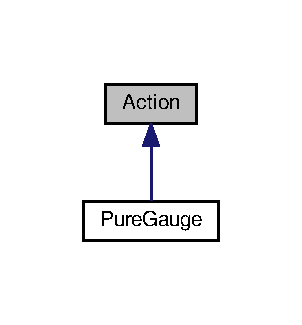
\includegraphics[width=145pt]{d7/d94/classAction__inherit__graph}
\end{center}
\end{figure}


Collaboration diagram for Action\+:\nopagebreak
\begin{figure}[H]
\begin{center}
\leavevmode
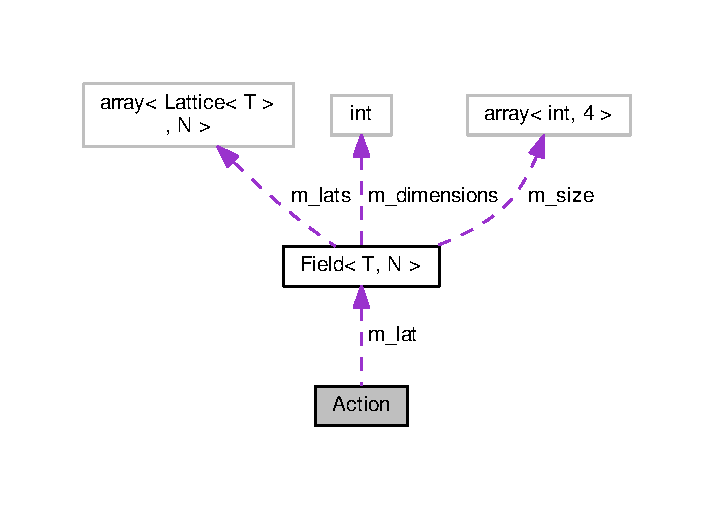
\includegraphics[width=343pt]{d7/dfc/classAction__coll__graph}
\end{center}
\end{figure}
\subsection*{Public Member Functions}
\begin{DoxyCompactItemize}
\item 
virtual double \hyperlink{classAction_ac0ea0d66e3ee4c7bdf0b478e613e5981}{compute} (int x, int y, int z, int t, int mu, \hyperlink{structSU3}{S\+U3} \&new\+Link)=0\hypertarget{classAction_ac0ea0d66e3ee4c7bdf0b478e613e5981}{}\label{classAction_ac0ea0d66e3ee4c7bdf0b478e613e5981}

\begin{DoxyCompactList}\small\item\em Computes the action difference around a given link for a suggested move. \end{DoxyCompactList}\item 
virtual void \hyperlink{classAction_ad6c5003169695d5cba0f69580040db50}{compute\+Staples} (int mu)=0\hypertarget{classAction_ad6c5003169695d5cba0f69580040db50}{}\label{classAction_ad6c5003169695d5cba0f69580040db50}

\begin{DoxyCompactList}\small\item\em Computes the sum of the staples around all links. \end{DoxyCompactList}\item 
virtual \hyperlink{classLattice}{Lattice}$<$ \hyperlink{structSU3}{S\+U3} $>$ \hyperlink{classAction_a722e4f88dda82440d0c6e19a43972b21}{compute\+Derivative} (int mu)=0\hypertarget{classAction_a722e4f88dda82440d0c6e19a43972b21}{}\label{classAction_a722e4f88dda82440d0c6e19a43972b21}

\begin{DoxyCompactList}\small\item\em Computes the derivative in a given direction around all links. \end{DoxyCompactList}\item 
void \hyperlink{classAction_a3c4e7cbcf64ae134fa86afd5d156b12b}{init\+Action} (\hyperlink{field_8h_afe80b127697eba6d6e7fbd8121c8d4ee}{Gluon\+Field} $\ast$field)
\begin{DoxyCompactList}\small\item\em Links the action to a given field and initializes. \end{DoxyCompactList}\end{DoxyCompactItemize}
\subsection*{Protected Attributes}
\begin{DoxyCompactItemize}
\item 
\hyperlink{field_8h_afe80b127697eba6d6e7fbd8121c8d4ee}{Gluon\+Field} $\ast$ \hyperlink{classAction_adfb7bb92099e0a908efaa4715e75fffd}{m\+\_\+lat} = nullptr\hypertarget{classAction_adfb7bb92099e0a908efaa4715e75fffd}{}\label{classAction_adfb7bb92099e0a908efaa4715e75fffd}

\begin{DoxyCompactList}\small\item\em The Gluon\+Field object the action is linked to. \end{DoxyCompactList}\end{DoxyCompactItemize}


\subsection{Detailed Description}
Prototype for the \hyperlink{classAction}{Action} class group. 

\begin{DoxyAuthor}{Author}
Giovanni Pederiva 
\end{DoxyAuthor}
\begin{DoxyVersion}{Version}
1.\+0 
\end{DoxyVersion}
\begin{DoxyDate}{Date}
2017-\/2018 
\end{DoxyDate}
\begin{DoxyCopyright}{Copyright}
M\+IT License.
\end{DoxyCopyright}
The \hyperlink{classAction}{Action} class is one of the key elements of the program. It specifies the acceptance of a Metropolis test and the evolution according to flow equations. It is of virtual type, so an implementation is always required. It mainly offers the possibility of retrieving the action around a single link or the derivative of the action around all links. 

Definition at line 54 of file action.\+h.



\subsection{Member Function Documentation}
\index{Action@{Action}!init\+Action@{init\+Action}}
\index{init\+Action@{init\+Action}!Action@{Action}}
\subsubsection[{\texorpdfstring{init\+Action(\+Gluon\+Field $\ast$field)}{initAction(GluonField *field)}}]{\setlength{\rightskip}{0pt plus 5cm}void Action\+::init\+Action (
\begin{DoxyParamCaption}
\item[{{\bf Gluon\+Field} $\ast$}]{lattice}
\end{DoxyParamCaption}
)}\hypertarget{classAction_a3c4e7cbcf64ae134fa86afd5d156b12b}{}\label{classAction_a3c4e7cbcf64ae134fa86afd5d156b12b}


Links the action to a given field and initializes. 

Links an action object to a Gluon\+Field object.


\begin{DoxyParams}{Parameters}
{\em lattice} & The gluonfield to link to the action instance. \\
\hline
\end{DoxyParams}


Definition at line 8 of file action.\+cpp.



The documentation for this class was generated from the following files\+:\begin{DoxyCompactItemize}
\item 
\hyperlink{action_8h}{action.\+h}\item 
action.\+cpp\end{DoxyCompactItemize}

\hypertarget{classApp}{}\section{App Class Reference}
\label{classApp}\index{App@{App}}


Inheritance diagram for App\+:
\nopagebreak
\begin{figure}[H]
\begin{center}
\leavevmode
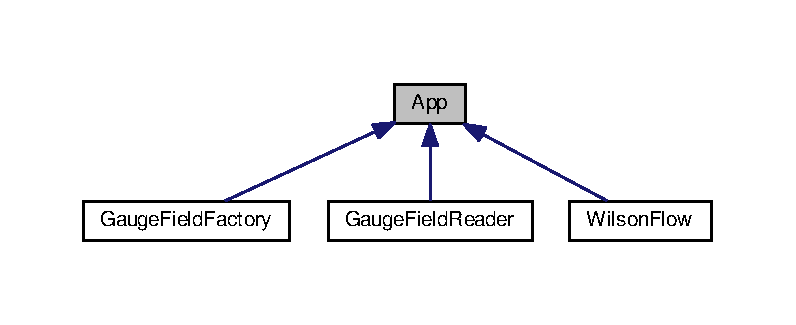
\includegraphics[width=350pt]{classApp__inherit__graph}
\end{center}
\end{figure}


Collaboration diagram for App\+:
\nopagebreak
\begin{figure}[H]
\begin{center}
\leavevmode
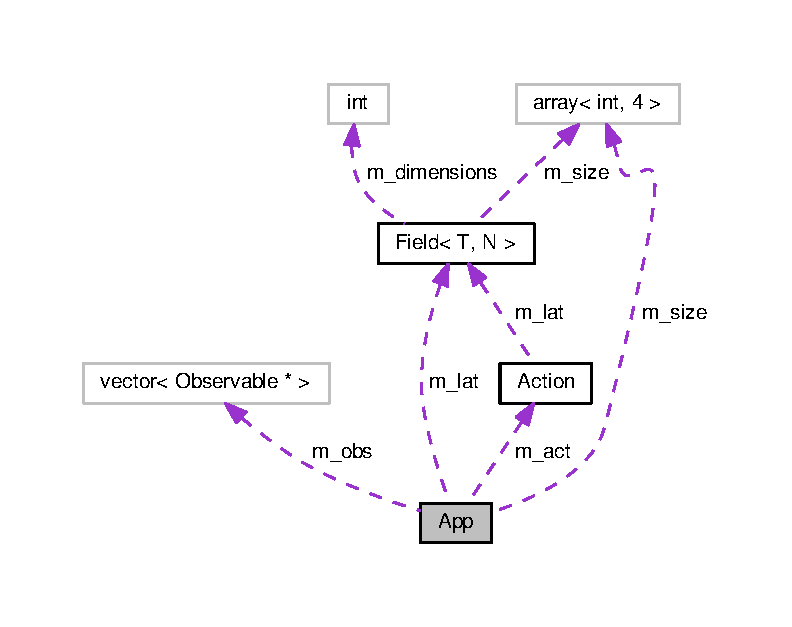
\includegraphics[width=350pt]{classApp__coll__graph}
\end{center}
\end{figure}
\subsection*{Public Member Functions}
\begin{DoxyCompactItemize}
\item 
void {\bfseries set\+Action} (\hyperlink{classAction}{Action} $\ast$action)\hypertarget{classApp_a521478e111127d2166d2e897b9900eb5}{}\label{classApp_a521478e111127d2166d2e897b9900eb5}

\item 
virtual void {\bfseries create\+Lattice} (std\+::array$<$ int, 4 $>$ lattice\+Size)\hypertarget{classApp_a8f35d6814a0306dd31c7c583f6c8d92c}{}\label{classApp_a8f35d6814a0306dd31c7c583f6c8d92c}

\item 
void {\bfseries add\+Observable} (\hyperlink{classObservable}{Observable} $\ast$observable)\hypertarget{classApp_a4796925a8a54cfe4456419b94160746e}{}\label{classApp_a4796925a8a54cfe4456419b94160746e}

\item 
virtual void {\bfseries execute} ()=0\hypertarget{classApp_a060dd95f437842171d448ac822dfa983}{}\label{classApp_a060dd95f437842171d448ac822dfa983}

\end{DoxyCompactItemize}
\subsection*{Protected Attributes}
\begin{DoxyCompactItemize}
\item 
\hyperlink{classAction}{Action} $\ast$ {\bfseries m\+\_\+act} = nullptr\hypertarget{classApp_a891ae68e54bb04fcf74579c62a8d5860}{}\label{classApp_a891ae68e54bb04fcf74579c62a8d5860}

\item 
\hyperlink{classField}{Gluon\+Field} $\ast$ {\bfseries m\+\_\+lat} = nullptr\hypertarget{classApp_a58776f77facca2185bf53974b05a7280}{}\label{classApp_a58776f77facca2185bf53974b05a7280}

\item 
std\+::array$<$ int, 4 $>$ {\bfseries m\+\_\+size}\hypertarget{classApp_a8ca118f6637bfd14129ba61f985876d7}{}\label{classApp_a8ca118f6637bfd14129ba61f985876d7}

\item 
std\+::vector$<$ \hyperlink{classObservable}{Observable} $\ast$ $>$ {\bfseries m\+\_\+obs}\hypertarget{classApp_af2803baf8aaf959201b28fb16a46a3d4}{}\label{classApp_af2803baf8aaf959201b28fb16a46a3d4}

\end{DoxyCompactItemize}


The documentation for this class was generated from the following files\+:\begin{DoxyCompactItemize}
\item 
/home/giovanni/\+Desktop/\+Lattice\+Yang\+Mills/include/\+Apps/app.\+h\item 
/home/giovanni/\+Desktop/\+Lattice\+Yang\+Mills/src/\+Apps/app.\+cpp\end{DoxyCompactItemize}

\hypertarget{classEnergyDensity}{}\section{Energy\+Density Class Reference}
\label{classEnergyDensity}\index{Energy\+Density@{Energy\+Density}}


Implementation of the Energy Density operator class.  




{\ttfamily \#include $<$energydensity.\+h$>$}



Inheritance diagram for Energy\+Density\+:\nopagebreak
\begin{figure}[H]
\begin{center}
\leavevmode
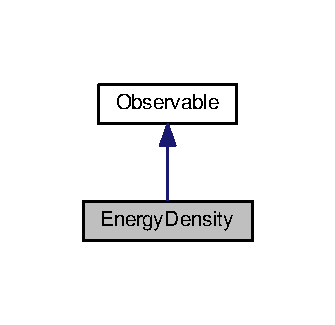
\includegraphics[width=161pt]{d2/d7e/classEnergyDensity__inherit__graph}
\end{center}
\end{figure}


Collaboration diagram for Energy\+Density\+:\nopagebreak
\begin{figure}[H]
\begin{center}
\leavevmode
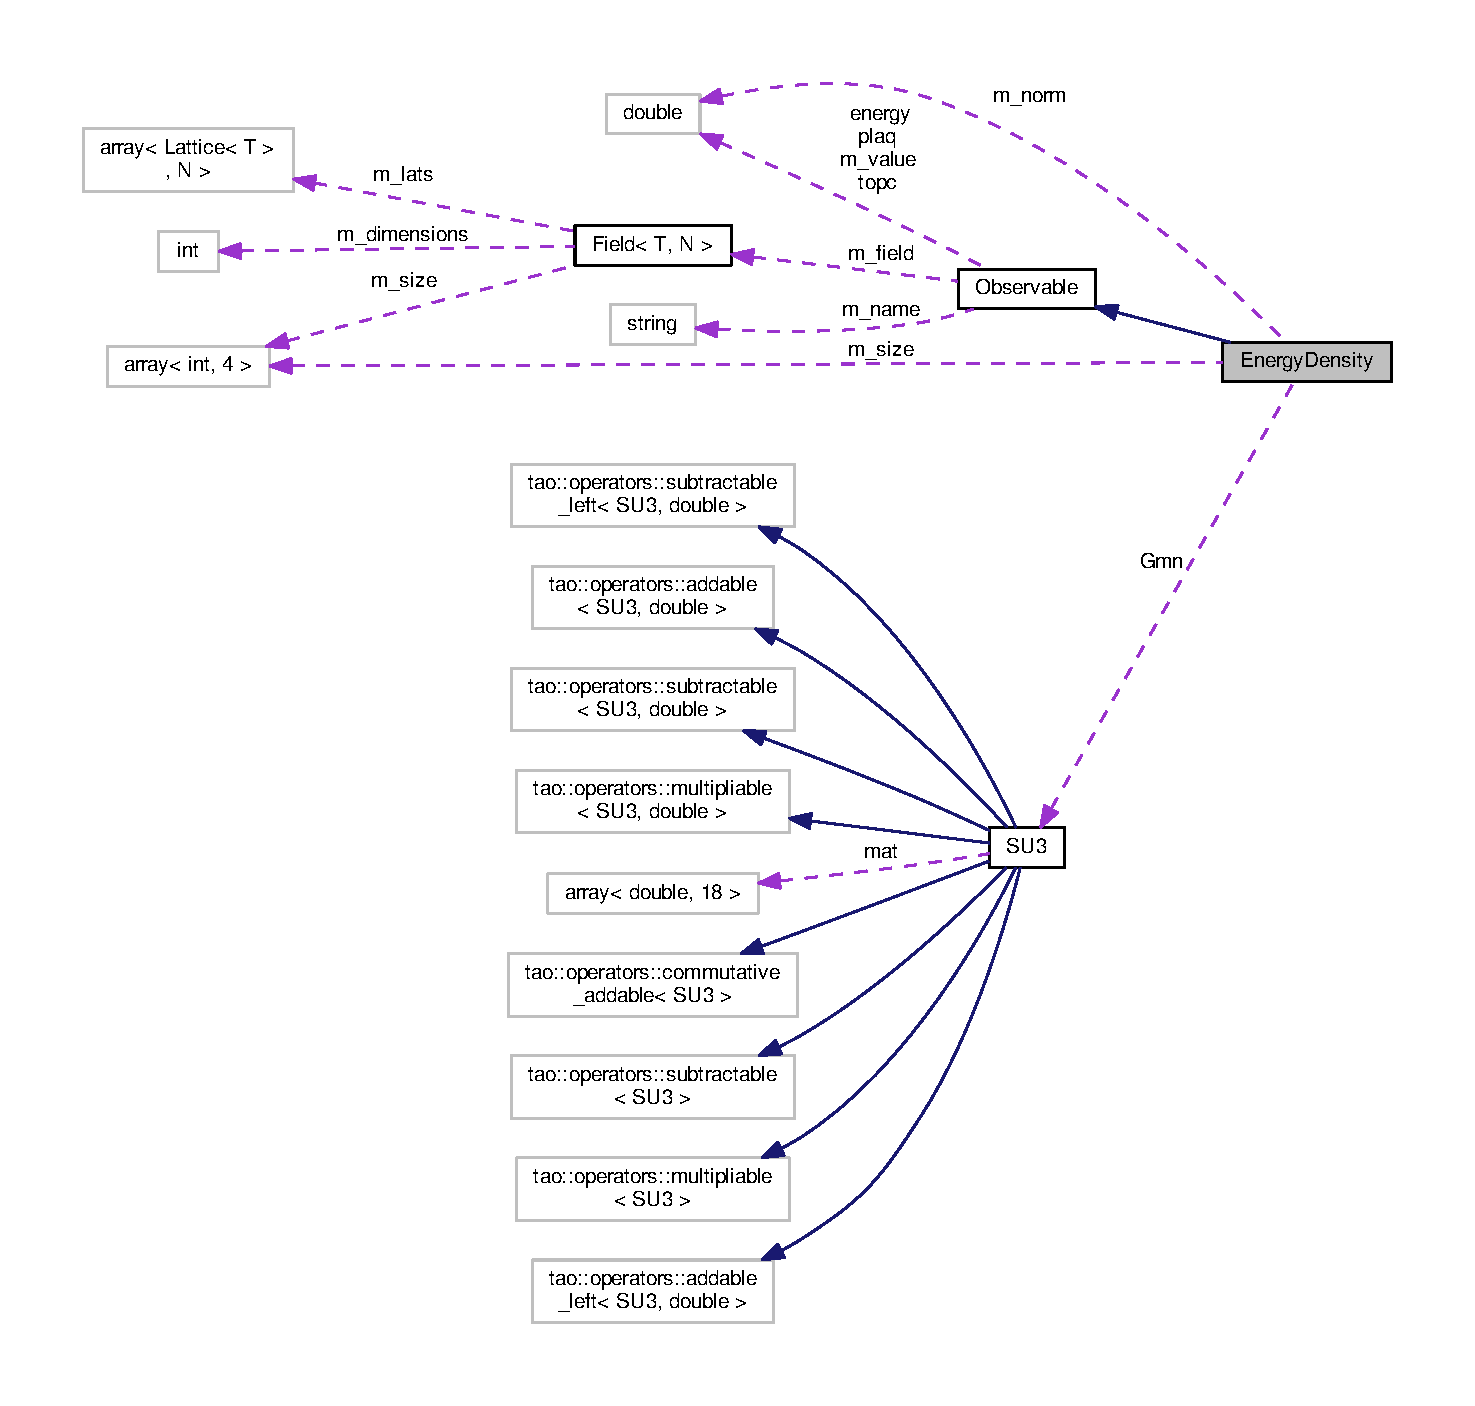
\includegraphics[width=350pt]{d5/d62/classEnergyDensity__coll__graph}
\end{center}
\end{figure}
\subsection*{Public Member Functions}
\begin{DoxyCompactItemize}
\item 
void {\bfseries init\+Observable} (\hyperlink{field_8h_afe80b127697eba6d6e7fbd8121c8d4ee}{Gluon\+Field} $\ast$lattice)\hypertarget{classEnergyDensity_ad076c85838b7d1e4d795655818369409}{}\label{classEnergyDensity_ad076c85838b7d1e4d795655818369409}

\item 
void {\bfseries compute} ()\hypertarget{classEnergyDensity_a8719af212e9534be4f23244c0ea85019}{}\label{classEnergyDensity_a8719af212e9534be4f23244c0ea85019}

\end{DoxyCompactItemize}
\subsection*{Private Attributes}
\begin{DoxyCompactItemize}
\item 
std\+::array$<$ int, 4 $>$ {\bfseries m\+\_\+size}\hypertarget{classEnergyDensity_a86486c6e6f1f4a0db45e33fe17c3eb84}{}\label{classEnergyDensity_a86486c6e6f1f4a0db45e33fe17c3eb84}

\item 
double {\bfseries m\+\_\+norm}\hypertarget{classEnergyDensity_a62b537a325d00c79646876d9178ddc22}{}\label{classEnergyDensity_a62b537a325d00c79646876d9178ddc22}

\item 
\hyperlink{structSU3}{S\+U3} {\bfseries Gmn}\hypertarget{classEnergyDensity_a7beebd4229b64e2829a4bf7fa708845f}{}\label{classEnergyDensity_a7beebd4229b64e2829a4bf7fa708845f}

\end{DoxyCompactItemize}
\subsection*{Additional Inherited Members}


\subsection{Detailed Description}
Implementation of the Energy Density operator class. 

\begin{DoxyAuthor}{Author}
Giovanni Pederiva 
\end{DoxyAuthor}
\begin{DoxyVersion}{Version}
0.\+1 
\end{DoxyVersion}
\begin{DoxyDate}{Date}
2017-\/2018 
\end{DoxyDate}
\begin{DoxyCopyright}{Copyright}
M\+IT License.
\end{DoxyCopyright}
Old implementation of the Energy Density operator class using the clover definition of the \hyperlink{classField}{Field} Stength Tensor 

Definition at line 52 of file energydensity.\+h.



The documentation for this class was generated from the following files\+:\begin{DoxyCompactItemize}
\item 
\hyperlink{energydensity_8h}{energydensity.\+h}\item 
energydensity.\+cpp\end{DoxyCompactItemize}

\hypertarget{classField}{}\section{Field$<$ T, N $>$ Class Template Reference}
\label{classField}\index{Field$<$ T, N $>$@{Field$<$ T, N $>$}}


Collaboration diagram for Field$<$ T, N $>$\+:\nopagebreak
\begin{figure}[H]
\begin{center}
\leavevmode
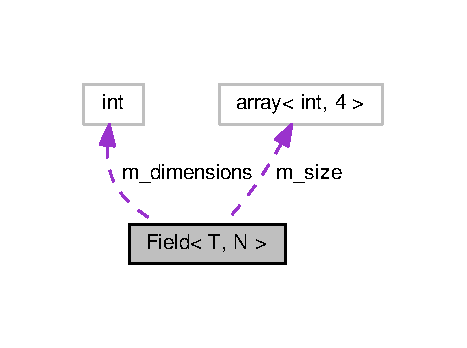
\includegraphics[width=224pt]{classField__coll__graph}
\end{center}
\end{figure}
\subsection*{Public Member Functions}
\begin{DoxyCompactItemize}
\item 
{\bfseries Field} (std\+::array$<$ int, 4 $>$ size)\hypertarget{classField_a25a5869a0faa4d33782cbe9f277f684f}{}\label{classField_a25a5869a0faa4d33782cbe9f277f684f}

\item 
\hyperlink{classLattice}{Lattice}$<$ T $>$ \& {\bfseries operator\mbox{[}$\,$\mbox{]}} (int mu)\hypertarget{classField_a2c9ffced05a0a329395b2d9bca338840}{}\label{classField_a2c9ffced05a0a329395b2d9bca338840}

\end{DoxyCompactItemize}
\subsection*{Public Attributes}
\begin{DoxyCompactItemize}
\item 
int {\bfseries m\+\_\+dimensions}\hypertarget{classField_ada68c99dbc291529adcbc58c87273403}{}\label{classField_ada68c99dbc291529adcbc58c87273403}

\item 
std\+::array$<$ int, 4 $>$ {\bfseries m\+\_\+size}\hypertarget{classField_ae6a537c53432f6631a5e6eb624deea90}{}\label{classField_ae6a537c53432f6631a5e6eb624deea90}

\end{DoxyCompactItemize}


The documentation for this class was generated from the following file\+:\begin{DoxyCompactItemize}
\item 
/home/giovanni/\+Desktop/\+Lattice\+Yang\+Mills/include/\+Math/field.\+h\end{DoxyCompactItemize}

\hypertarget{classGaugeFieldFactory}{}\section{Gauge\+Field\+Factory Class Reference}
\label{classGaugeFieldFactory}\index{Gauge\+Field\+Factory@{Gauge\+Field\+Factory}}


Inheritance diagram for Gauge\+Field\+Factory\+:\nopagebreak
\begin{figure}[H]
\begin{center}
\leavevmode
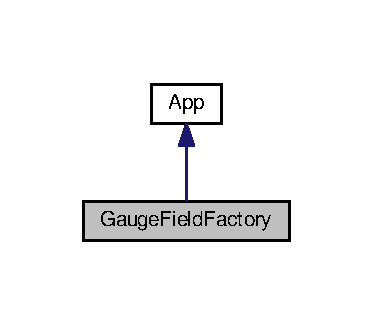
\includegraphics[width=179pt]{da/deb/classGaugeFieldFactory__inherit__graph}
\end{center}
\end{figure}


Collaboration diagram for Gauge\+Field\+Factory\+:
\nopagebreak
\begin{figure}[H]
\begin{center}
\leavevmode
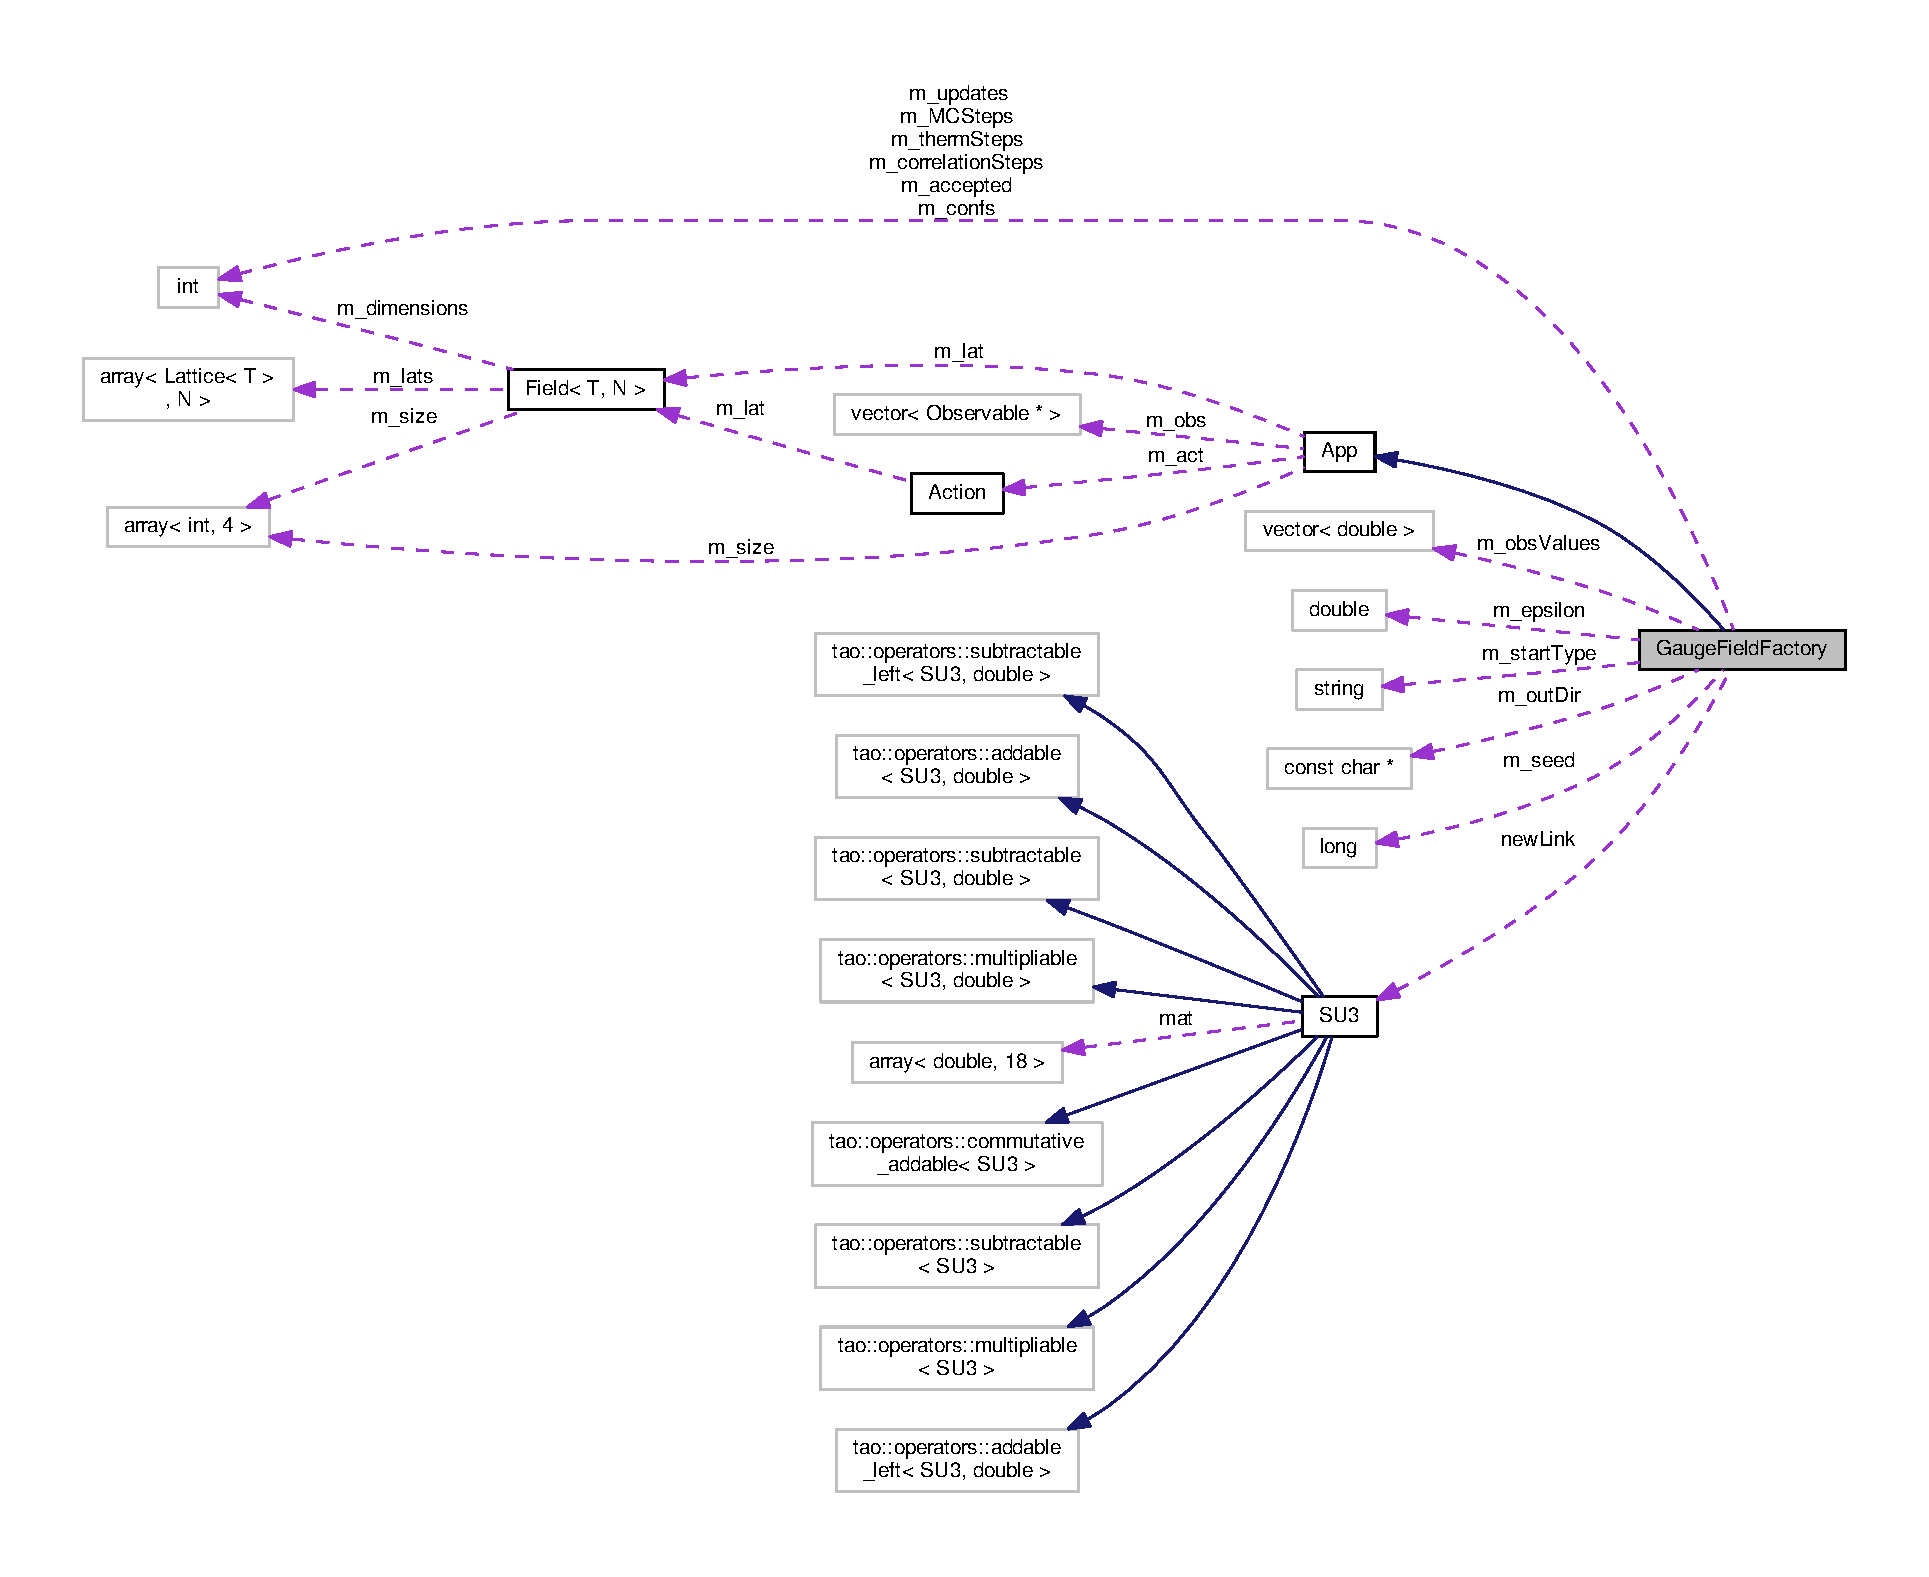
\includegraphics[width=350pt]{df/dd0/classGaugeFieldFactory__coll__graph}
\end{center}
\end{figure}
\subsection*{Public Member Functions}
\begin{DoxyCompactItemize}
\item 
{\bfseries Gauge\+Field\+Factory} (int M\+C\+Steps, int therm\+Steps, int N\+Conf, double epsilon, std\+::string start\+Type)\hypertarget{classGaugeFieldFactory_ab4de95086757f8dad2bb82225990798c}{}\label{classGaugeFieldFactory_ab4de95086757f8dad2bb82225990798c}

\item 
void {\bfseries generate\+Configurations} ()\hypertarget{classGaugeFieldFactory_a44af20883686c17d5cc02b0017981a00}{}\label{classGaugeFieldFactory_a44af20883686c17d5cc02b0017981a00}

\item 
std\+::vector$<$ double $>$ \& {\bfseries get\+Obs\+Values} ()\hypertarget{classGaugeFieldFactory_a3455c32bf0d8e97c5b20a6372b108a42}{}\label{classGaugeFieldFactory_a3455c32bf0d8e97c5b20a6372b108a42}

\item 
void {\bfseries execute} ()\hypertarget{classGaugeFieldFactory_ae71b983ead390226ddad5d0f13aba0c6}{}\label{classGaugeFieldFactory_ae71b983ead390226ddad5d0f13aba0c6}

\end{DoxyCompactItemize}
\subsection*{Private Member Functions}
\begin{DoxyCompactItemize}
\item 
void {\bfseries initialize} ()\hypertarget{classGaugeFieldFactory_a3b7b0bc33811c149c85b595f5c724ddb}{}\label{classGaugeFieldFactory_a3b7b0bc33811c149c85b595f5c724ddb}

\item 
void {\bfseries M\+C\+Update} ()\hypertarget{classGaugeFieldFactory_a23a45078029941f5e5dd2d699935d38b}{}\label{classGaugeFieldFactory_a23a45078029941f5e5dd2d699935d38b}

\item 
void {\bfseries update\+Link} (int x, int y, int z, int t, int mu)\hypertarget{classGaugeFieldFactory_ac58103157c9d39daa4819e2f9e8b7024}{}\label{classGaugeFieldFactory_ac58103157c9d39daa4819e2f9e8b7024}

\item 
void {\bfseries compute\+Observables} ()\hypertarget{classGaugeFieldFactory_a70fc0cc23088b190f35c56885762812a}{}\label{classGaugeFieldFactory_a70fc0cc23088b190f35c56885762812a}

\item 
void {\bfseries thermalize} ()\hypertarget{classGaugeFieldFactory_a18bc263a1dac26f0147063c33e33a518}{}\label{classGaugeFieldFactory_a18bc263a1dac26f0147063c33e33a518}

\item 
void {\bfseries sample\+Conf} ()\hypertarget{classGaugeFieldFactory_a37df236572b4c1adf1a00d3d1374621a}{}\label{classGaugeFieldFactory_a37df236572b4c1adf1a00d3d1374621a}

\item 
void {\bfseries thermalize\+Time} ()\hypertarget{classGaugeFieldFactory_aaacc047577bbb5d0fcb790525d8ff958}{}\label{classGaugeFieldFactory_aaacc047577bbb5d0fcb790525d8ff958}

\item 
void {\bfseries sample\+Conf\+Time} ()\hypertarget{classGaugeFieldFactory_adc5d83defde9295cdc32c9c4ec59af59}{}\label{classGaugeFieldFactory_adc5d83defde9295cdc32c9c4ec59af59}

\end{DoxyCompactItemize}
\subsection*{Private Attributes}
\begin{DoxyCompactItemize}
\item 
std\+::vector$<$ double $>$ {\bfseries m\+\_\+obs\+Values}\hypertarget{classGaugeFieldFactory_ab6d5d1f77e9731709899bf68a13d6b66}{}\label{classGaugeFieldFactory_ab6d5d1f77e9731709899bf68a13d6b66}

\item 
int {\bfseries m\+\_\+\+M\+C\+Steps}\hypertarget{classGaugeFieldFactory_acdb2e28a0996b989e90507aeaa779358}{}\label{classGaugeFieldFactory_acdb2e28a0996b989e90507aeaa779358}

\item 
int {\bfseries m\+\_\+correlation\+Steps}\hypertarget{classGaugeFieldFactory_a4766228f02c8e75b98c36d9b3231a13d}{}\label{classGaugeFieldFactory_a4766228f02c8e75b98c36d9b3231a13d}

\item 
int {\bfseries m\+\_\+therm\+Steps}\hypertarget{classGaugeFieldFactory_aa4426a1d60452c4882556224262ab447}{}\label{classGaugeFieldFactory_aa4426a1d60452c4882556224262ab447}

\item 
int {\bfseries m\+\_\+confs}\hypertarget{classGaugeFieldFactory_a08f5104224cb00356243d3a7deee1331}{}\label{classGaugeFieldFactory_a08f5104224cb00356243d3a7deee1331}

\item 
std\+::string {\bfseries m\+\_\+start\+Type}\hypertarget{classGaugeFieldFactory_a270a1a8e7995761b26d41cf2217fd180}{}\label{classGaugeFieldFactory_a270a1a8e7995761b26d41cf2217fd180}

\item 
double {\bfseries m\+\_\+epsilon}\hypertarget{classGaugeFieldFactory_a615f5d961e3326339a6e39d11c1fffea}{}\label{classGaugeFieldFactory_a615f5d961e3326339a6e39d11c1fffea}

\item 
long int {\bfseries m\+\_\+accepted} = 0\hypertarget{classGaugeFieldFactory_ae1910e40b9471b9722e6392d1f4665cc}{}\label{classGaugeFieldFactory_ae1910e40b9471b9722e6392d1f4665cc}

\item 
long int {\bfseries m\+\_\+updates} = 0\hypertarget{classGaugeFieldFactory_a4e1118e49b8ead095c6ceead1a337943}{}\label{classGaugeFieldFactory_a4e1118e49b8ead095c6ceead1a337943}

\item 
long {\bfseries m\+\_\+seed}\hypertarget{classGaugeFieldFactory_a56f0e062cd0cb3d73b487891ccb67462}{}\label{classGaugeFieldFactory_a56f0e062cd0cb3d73b487891ccb67462}

\item 
const char $\ast$ {\bfseries m\+\_\+out\+Dir}\hypertarget{classGaugeFieldFactory_ad231575f1bf834b20ff5e948331b748c}{}\label{classGaugeFieldFactory_ad231575f1bf834b20ff5e948331b748c}

\item 
\hyperlink{structSU3}{S\+U3} {\bfseries new\+Link}\hypertarget{classGaugeFieldFactory_af15971c810e2e4cee7de71e9560b16fc}{}\label{classGaugeFieldFactory_af15971c810e2e4cee7de71e9560b16fc}

\end{DoxyCompactItemize}
\subsection*{Additional Inherited Members}


The documentation for this class was generated from the following files\+:\begin{DoxyCompactItemize}
\item 
gaugefieldfactory.\+h\item 
gaugefieldfactory.\+cpp\end{DoxyCompactItemize}

\hypertarget{classGaugeFieldReader}{}\section{Gauge\+Field\+Reader Class Reference}
\label{classGaugeFieldReader}\index{Gauge\+Field\+Reader@{Gauge\+Field\+Reader}}


Inheritance diagram for Gauge\+Field\+Reader\+:\nopagebreak
\begin{figure}[H]
\begin{center}
\leavevmode
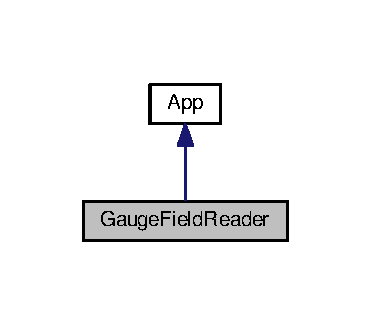
\includegraphics[width=178pt]{d8/dcd/classGaugeFieldReader__inherit__graph}
\end{center}
\end{figure}


Collaboration diagram for Gauge\+Field\+Reader\+:
\nopagebreak
\begin{figure}[H]
\begin{center}
\leavevmode
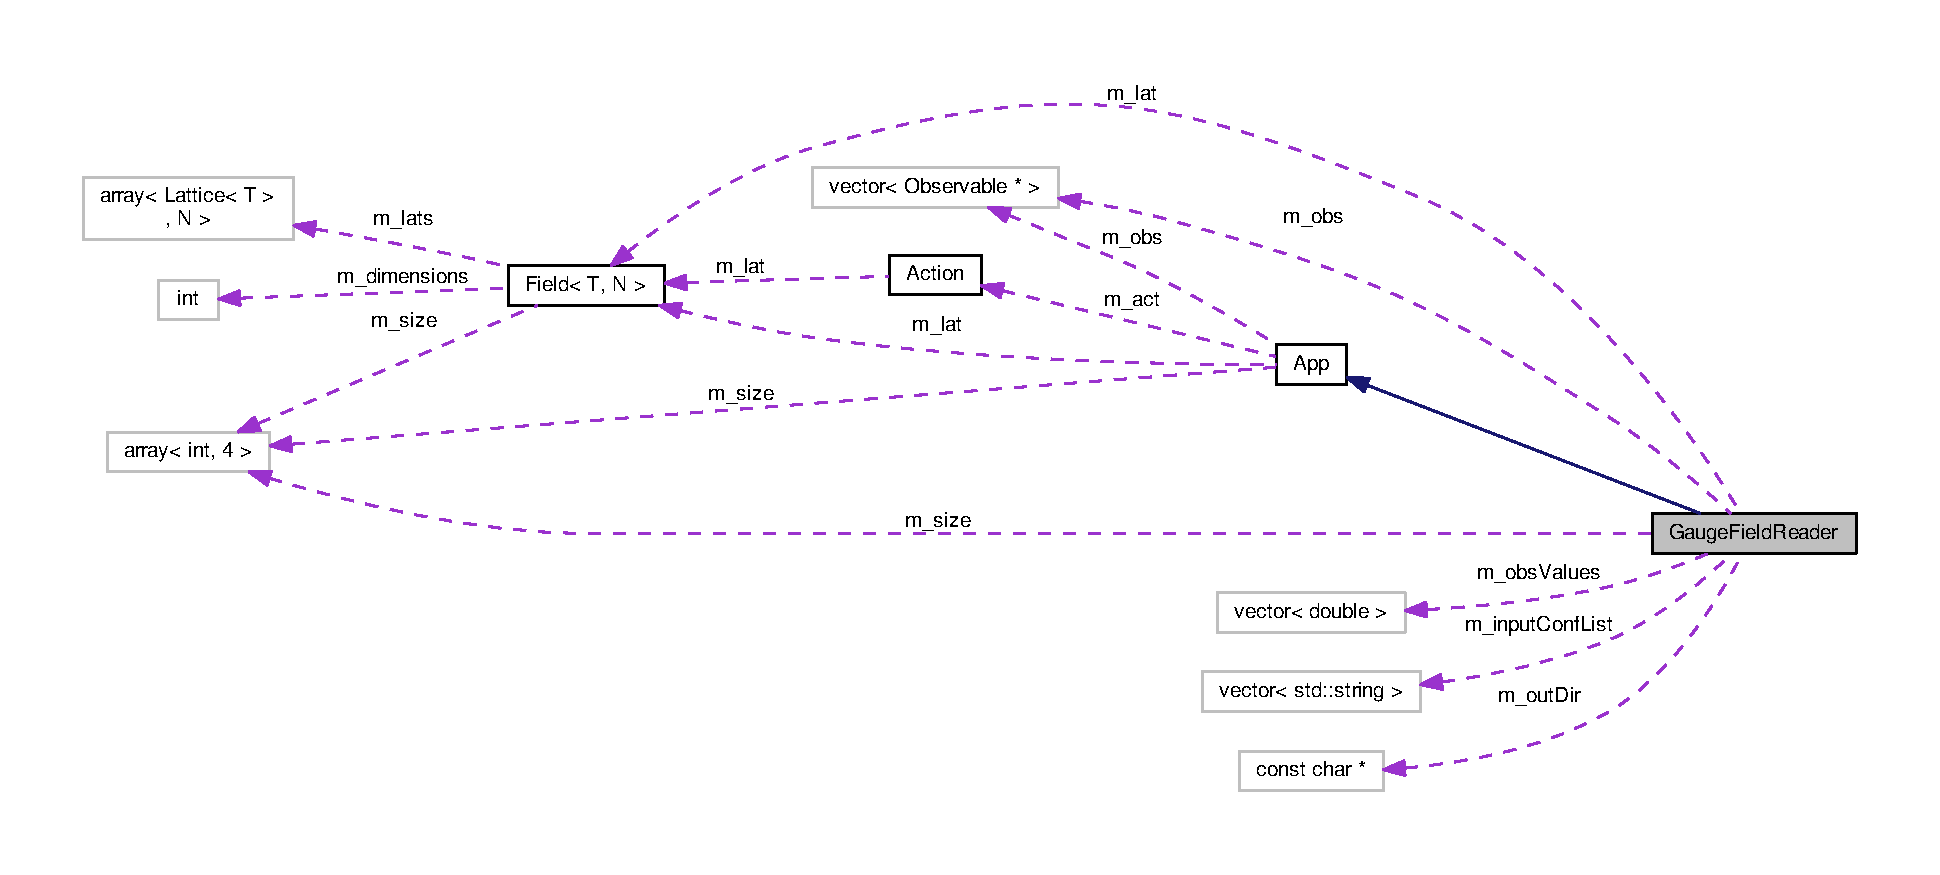
\includegraphics[width=350pt]{d7/d2a/classGaugeFieldReader__coll__graph}
\end{center}
\end{figure}
\subsection*{Public Member Functions}
\begin{DoxyCompactItemize}
\item 
void {\bfseries init\+G\+FR} ()\hypertarget{classGaugeFieldReader_aa4eac4656319ffb5d397dc6dd6b4f426}{}\label{classGaugeFieldReader_aa4eac4656319ffb5d397dc6dd6b4f426}

\item 
void {\bfseries sample\+Configurations} ()\hypertarget{classGaugeFieldReader_acc45c7e6e91ccb4e1b7f8d1f65104153}{}\label{classGaugeFieldReader_acc45c7e6e91ccb4e1b7f8d1f65104153}

\item 
void {\bfseries add\+Observable} (\hyperlink{classObservable}{Observable} $\ast$observable)\hypertarget{classGaugeFieldReader_af795e0891c276b0a6c8d8ade159df3b8}{}\label{classGaugeFieldReader_af795e0891c276b0a6c8d8ade159df3b8}

\item 
const char $\ast$ {\bfseries get\+Out\+Dir} ()\hypertarget{classGaugeFieldReader_a015c7811098f42d98b7a9d5f3b52d8b4}{}\label{classGaugeFieldReader_a015c7811098f42d98b7a9d5f3b52d8b4}

\item 
std\+::array$<$ int, 4 $>$ \& {\bfseries get\+Size} ()\hypertarget{classGaugeFieldReader_a2c7cc1114b6442acdb3112409e50792f}{}\label{classGaugeFieldReader_a2c7cc1114b6442acdb3112409e50792f}

\item 
std\+::vector$<$ double $>$ \& {\bfseries get\+Obs\+Values} ()\hypertarget{classGaugeFieldReader_a470083eb93cd916886d1ea68091ee728}{}\label{classGaugeFieldReader_a470083eb93cd916886d1ea68091ee728}

\item 
std\+::vector$<$ \hyperlink{classObservable}{Observable} $\ast$ $>$ \& {\bfseries get\+Obs} ()\hypertarget{classGaugeFieldReader_a3326dd6abb58a608a387e7e91a1ed0cc}{}\label{classGaugeFieldReader_a3326dd6abb58a608a387e7e91a1ed0cc}

\item 
void {\bfseries execute} ()\hypertarget{classGaugeFieldReader_af410d62a4f0e146db40111d5be672264}{}\label{classGaugeFieldReader_af410d62a4f0e146db40111d5be672264}

\end{DoxyCompactItemize}
\subsection*{Private Attributes}
\begin{DoxyCompactItemize}
\item 
\hyperlink{classField}{Gluon\+Field} $\ast$ {\bfseries m\+\_\+lat} = nullptr\hypertarget{classGaugeFieldReader_a5463d397d298c410b7a22d5f5b4a479e}{}\label{classGaugeFieldReader_a5463d397d298c410b7a22d5f5b4a479e}

\item 
std\+::vector$<$ \hyperlink{classObservable}{Observable} $\ast$ $>$ {\bfseries m\+\_\+obs}\hypertarget{classGaugeFieldReader_a754535c031598fef45833888e9979fe1}{}\label{classGaugeFieldReader_a754535c031598fef45833888e9979fe1}

\item 
std\+::vector$<$ double $>$ {\bfseries m\+\_\+obs\+Values}\hypertarget{classGaugeFieldReader_aeda178d621e12f56a9c377385bb1be0e}{}\label{classGaugeFieldReader_aeda178d621e12f56a9c377385bb1be0e}

\item 
std\+::vector$<$ std\+::string $>$ {\bfseries m\+\_\+input\+Conf\+List}\hypertarget{classGaugeFieldReader_a92c2a16c7ea8d99a156f8bf721cbd3cf}{}\label{classGaugeFieldReader_a92c2a16c7ea8d99a156f8bf721cbd3cf}

\item 
std\+::array$<$ int, 4 $>$ {\bfseries m\+\_\+size}\hypertarget{classGaugeFieldReader_ae82df049657776beb85fc3bbb36dad4e}{}\label{classGaugeFieldReader_ae82df049657776beb85fc3bbb36dad4e}

\item 
const char $\ast$ {\bfseries m\+\_\+out\+Dir}\hypertarget{classGaugeFieldReader_a2094749f83fd803ccc01e477aaa482e7}{}\label{classGaugeFieldReader_a2094749f83fd803ccc01e477aaa482e7}

\end{DoxyCompactItemize}
\subsection*{Additional Inherited Members}


The documentation for this class was generated from the following files\+:\begin{DoxyCompactItemize}
\item 
gaugefieldreader.\+h\item 
gaugefieldreader.\+cpp\end{DoxyCompactItemize}

\hypertarget{classLatticeIO_1_1InputConf}{}\section{Lattice\+IO\+:\+:Input\+Conf Class Reference}
\label{classLatticeIO_1_1InputConf}\index{Lattice\+I\+O\+::\+Input\+Conf@{Lattice\+I\+O\+::\+Input\+Conf}}


Class for reding lattices from binary files.  




{\ttfamily \#include $<$inputconf.\+h$>$}



Collaboration diagram for Lattice\+IO\+:\+:Input\+Conf\+:\nopagebreak
\begin{figure}[H]
\begin{center}
\leavevmode
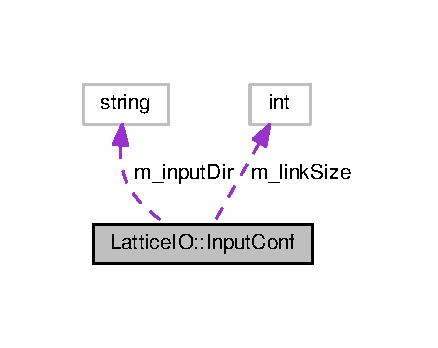
\includegraphics[width=210pt]{d0/d42/classLatticeIO_1_1InputConf__coll__graph}
\end{center}
\end{figure}
\subsection*{Static Public Member Functions}
\begin{DoxyCompactItemize}
\item 
static void \hyperlink{classLatticeIO_1_1InputConf_a70d70bfdc0252ddaa3d2bcd472590982}{read\+Conf} (\hyperlink{classField}{Gluon\+Field} \&lattice, int conf\+Num)\hypertarget{classLatticeIO_1_1InputConf_a70d70bfdc0252ddaa3d2bcd472590982}{}\label{classLatticeIO_1_1InputConf_a70d70bfdc0252ddaa3d2bcd472590982}

\begin{DoxyCompactList}\small\item\em Reads a binary file from a int marker for the name. \end{DoxyCompactList}\item 
static void \hyperlink{classLatticeIO_1_1InputConf_aed71fc3df1e2a9999e4466b5eefdf723}{read\+Conf} (\hyperlink{classField}{Gluon\+Field} \&lattice, const char $\ast$input\+File)\hypertarget{classLatticeIO_1_1InputConf_aed71fc3df1e2a9999e4466b5eefdf723}{}\label{classLatticeIO_1_1InputConf_aed71fc3df1e2a9999e4466b5eefdf723}

\begin{DoxyCompactList}\small\item\em Reads a binary file given its path into a lattice object. \end{DoxyCompactList}\item 
static void \hyperlink{classLatticeIO_1_1InputConf_a0ea75c17916f8ce880d02a13b127cea8}{read\+Sub\+Lattice} (\hyperlink{classField}{Gluon\+Field} \&lattice, int conf\+Num)\hypertarget{classLatticeIO_1_1InputConf_a0ea75c17916f8ce880d02a13b127cea8}{}\label{classLatticeIO_1_1InputConf_a0ea75c17916f8ce880d02a13b127cea8}

\begin{DoxyCompactList}\small\item\em Reads one binary file for each processor, assuming it is split. \end{DoxyCompactList}\item 
static void \hyperlink{classLatticeIO_1_1InputConf_a49a84ce29fc32889d6c356c3afd09b71}{set\+Input\+Dir} (std\+::string input\+Dir)\hypertarget{classLatticeIO_1_1InputConf_a49a84ce29fc32889d6c356c3afd09b71}{}\label{classLatticeIO_1_1InputConf_a49a84ce29fc32889d6c356c3afd09b71}

\begin{DoxyCompactList}\small\item\em Sets the input directory. \end{DoxyCompactList}\item 
static void \hyperlink{classLatticeIO_1_1InputConf_a16b06fe98129e3c1e80879fa9cad43a9}{get\+Input\+List} (std\+::vector$<$ std\+::string $>$ \&input\+Conf\+List)\hypertarget{classLatticeIO_1_1InputConf_a16b06fe98129e3c1e80879fa9cad43a9}{}\label{classLatticeIO_1_1InputConf_a16b06fe98129e3c1e80879fa9cad43a9}

\begin{DoxyCompactList}\small\item\em Returns a list of all valid input files in a the input directory. \end{DoxyCompactList}\end{DoxyCompactItemize}
\subsection*{Static Private Attributes}
\begin{DoxyCompactItemize}
\item 
static int \hyperlink{classLatticeIO_1_1InputConf_a1f6a72c39487a0b44cacd27b15a0df0d}{m\+\_\+link\+Size} = 18 $\ast$ sizeof(double)\hypertarget{classLatticeIO_1_1InputConf_a1f6a72c39487a0b44cacd27b15a0df0d}{}\label{classLatticeIO_1_1InputConf_a1f6a72c39487a0b44cacd27b15a0df0d}

\begin{DoxyCompactList}\small\item\em Contains the size in bytes of a 4 links on a lattice site. \end{DoxyCompactList}\item 
static std\+::string \hyperlink{classLatticeIO_1_1InputConf_ac2dcaeda7ddb006f1446b53f5ec6f168}{m\+\_\+input\+Dir}\hypertarget{classLatticeIO_1_1InputConf_ac2dcaeda7ddb006f1446b53f5ec6f168}{}\label{classLatticeIO_1_1InputConf_ac2dcaeda7ddb006f1446b53f5ec6f168}

\begin{DoxyCompactList}\small\item\em The path of the input directory. \end{DoxyCompactList}\end{DoxyCompactItemize}


\subsection{Detailed Description}
Class for reding lattices from binary files. 

\begin{DoxyAuthor}{Author}
Giovanni Pederiva 
\end{DoxyAuthor}
\begin{DoxyVersion}{Version}
1.\+0 
\end{DoxyVersion}
\begin{DoxyDate}{Date}
2017-\/2018 
\end{DoxyDate}
\begin{DoxyCopyright}{Copyright}
M\+IT License.
\end{DoxyCopyright}
This object allows reading of Gluon\+Field objects as binary files. It uses M\+PI routines for handling a single input file with multiple processors. 

The documentation for this class was generated from the following files\+:\begin{DoxyCompactItemize}
\item 
\hyperlink{inputconf_8h}{inputconf.\+h}\item 
inputconf.\+cpp\end{DoxyCompactItemize}

\hypertarget{classLattice}{}\section{Lattice$<$ T $>$ Class Template Reference}
\label{classLattice}\index{Lattice$<$ T $>$@{Lattice$<$ T $>$}}


Collaboration diagram for Lattice$<$ T $>$\+:
\nopagebreak
\begin{figure}[H]
\begin{center}
\leavevmode
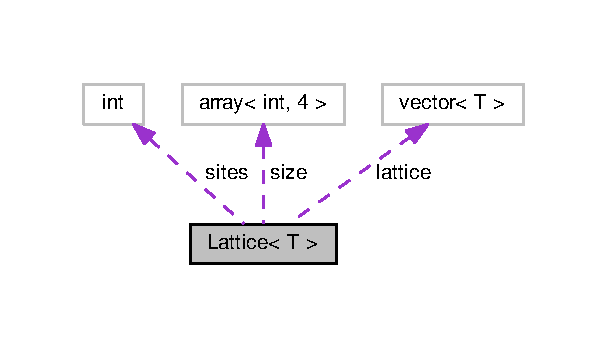
\includegraphics[width=292pt]{classLattice__coll__graph}
\end{center}
\end{figure}
\subsection*{Public Member Functions}
\begin{DoxyCompactItemize}
\item 
{\bfseries Lattice} (const \hyperlink{classLattice}{Lattice} \&other) noexcept\hypertarget{classLattice_a329f8bb4934a16dde20245e5aed1e0f2}{}\label{classLattice_a329f8bb4934a16dde20245e5aed1e0f2}

\item 
{\bfseries Lattice} (\hyperlink{classLattice}{Lattice} \&\&other) noexcept\hypertarget{classLattice_ac515062dd08174cfd300cb7ae82c1131}{}\label{classLattice_ac515062dd08174cfd300cb7ae82c1131}

\item 
{\bfseries Lattice} (std\+::array$<$ int, 4 $>$ size\+Array)\hypertarget{classLattice_a9583bced9172a01d6abb839dc1bea8a4}{}\label{classLattice_a9583bced9172a01d6abb839dc1bea8a4}

\item 
void {\bfseries allocate} (std\+::array$<$ int, 4 $>$ size\+Array)\hypertarget{classLattice_a34d4aba6e3440624d7a78f3de5604bbe}{}\label{classLattice_a34d4aba6e3440624d7a78f3de5604bbe}

\item 
T \& {\bfseries at} (int x, int y, int z, int t)\hypertarget{classLattice_a9345ef22de8cd40304ffaa24bbf84e57}{}\label{classLattice_a9345ef22de8cd40304ffaa24bbf84e57}

\item 
T \& {\bfseries at} (const std\+::vector$<$ int $>$ \&site)\hypertarget{classLattice_a505c50837cfcda18a1f26837ba487d1b}{}\label{classLattice_a505c50837cfcda18a1f26837ba487d1b}

\item 
T \& {\bfseries at} (const std\+::array$<$ int, 4 $>$ \&site)\hypertarget{classLattice_a2885da42d927704c9a465f31d4809302}{}\label{classLattice_a2885da42d927704c9a465f31d4809302}

\item 
T \& {\bfseries at} (int i)\hypertarget{classLattice_a7edbcfba94b2c85c8a73eef6c8b4969c}{}\label{classLattice_a7edbcfba94b2c85c8a73eef6c8b4969c}

\item 
const T \& {\bfseries at} (int x, int y, int z, int t) const \hypertarget{classLattice_a0f68df177d44035f352c097dc59d7b69}{}\label{classLattice_a0f68df177d44035f352c097dc59d7b69}

\item 
const T \& {\bfseries at} (const std\+::vector$<$ int $>$ \&site) const \hypertarget{classLattice_a75069863087489b2977074cd52ed8f73}{}\label{classLattice_a75069863087489b2977074cd52ed8f73}

\item 
const T \& {\bfseries at} (const std\+::array$<$ int, 4 $>$ \&site) const \hypertarget{classLattice_a5841feb3f15f2ee81888203dcdb49703}{}\label{classLattice_a5841feb3f15f2ee81888203dcdb49703}

\item 
const T \& {\bfseries at} (int i) const \hypertarget{classLattice_af9c0f4cc4d74390b488a8f5a8c766934}{}\label{classLattice_af9c0f4cc4d74390b488a8f5a8c766934}

\item 
\hyperlink{classLattice}{Lattice} \& {\bfseries operator=} (const \hyperlink{classLattice}{Lattice} \&other) noexcept\hypertarget{classLattice_a70008d522e42d75886c1398e3a00a77d}{}\label{classLattice_a70008d522e42d75886c1398e3a00a77d}

\item 
\hyperlink{classLattice}{Lattice} \& {\bfseries operator=} (\hyperlink{classLattice}{Lattice} \&\&other) noexcept\hypertarget{classLattice_aee5bfa33b3dc9fb895972637214b4ad5}{}\label{classLattice_aee5bfa33b3dc9fb895972637214b4ad5}

\item 
\hyperlink{classLattice}{Lattice} \& {\bfseries operator+=} (const \hyperlink{classLattice}{Lattice} \&other) noexcept\hypertarget{classLattice_a8287a398257dab76e3f7445a27cd2d85}{}\label{classLattice_a8287a398257dab76e3f7445a27cd2d85}

\item 
\hyperlink{classLattice}{Lattice} \& {\bfseries operator+=} (\hyperlink{classLattice}{Lattice} \&\&other) noexcept\hypertarget{classLattice_a8a524b7c0b8f2e5e95c1e08b7fae60e7}{}\label{classLattice_a8a524b7c0b8f2e5e95c1e08b7fae60e7}

\item 
\hyperlink{classLattice}{Lattice} \& {\bfseries operator-\/=} (const \hyperlink{classLattice}{Lattice} \&other) noexcept\hypertarget{classLattice_aadebcf9c9b2afe5c2216fe63c27110a7}{}\label{classLattice_aadebcf9c9b2afe5c2216fe63c27110a7}

\item 
\hyperlink{classLattice}{Lattice} \& {\bfseries operator-\/=} (\hyperlink{classLattice}{Lattice} \&\&other) noexcept\hypertarget{classLattice_a848894fff4a8443567d203840ecb183d}{}\label{classLattice_a848894fff4a8443567d203840ecb183d}

\item 
\hyperlink{classLattice}{Lattice} \& {\bfseries operator$\ast$=} (const \hyperlink{classLattice}{Lattice} \&other) noexcept\hypertarget{classLattice_a8bbf23e229a86a1ac20d4d799411bf7e}{}\label{classLattice_a8bbf23e229a86a1ac20d4d799411bf7e}

\item 
\hyperlink{classLattice}{Lattice} \& {\bfseries operator$\ast$=} (\hyperlink{classLattice}{Lattice} \&\&other) noexcept\hypertarget{classLattice_acdc58066b4aa455eb6579bed8f4d2e6b}{}\label{classLattice_acdc58066b4aa455eb6579bed8f4d2e6b}

\item 
\hyperlink{classLattice}{Lattice} \& {\bfseries operator+=} (double scalar) noexcept\hypertarget{classLattice_a63b58993c23eb173009d8f47d31c9446}{}\label{classLattice_a63b58993c23eb173009d8f47d31c9446}

\item 
\hyperlink{classLattice}{Lattice} \& {\bfseries operator-\/=} (double scalar) noexcept\hypertarget{classLattice_a7bef43f0f3d27355c68d7b6cf945cd74}{}\label{classLattice_a7bef43f0f3d27355c68d7b6cf945cd74}

\item 
\hyperlink{classLattice}{Lattice} \& {\bfseries operator$\ast$=} (double scalar) noexcept\hypertarget{classLattice_a03c24714fb6d662c3b65d099b6538e41}{}\label{classLattice_a03c24714fb6d662c3b65d099b6538e41}

\end{DoxyCompactItemize}
\subsection*{Public Attributes}
\begin{DoxyCompactItemize}
\item 
std\+::vector$<$ T $>$ {\bfseries lattice}\hypertarget{classLattice_af008a9fb4d68830116171ad510dac00d}{}\label{classLattice_af008a9fb4d68830116171ad510dac00d}

\item 
std\+::array$<$ int, 4 $>$ {\bfseries size}\hypertarget{classLattice_a24efa6069bfbc8efceec45aa4048310b}{}\label{classLattice_a24efa6069bfbc8efceec45aa4048310b}

\item 
int {\bfseries sites}\hypertarget{classLattice_a445869fa94228c717650aefa85d02567}{}\label{classLattice_a445869fa94228c717650aefa85d02567}

\end{DoxyCompactItemize}
\subsection*{Friends}
\begin{DoxyCompactItemize}
\item 
\hyperlink{classLattice}{Lattice} {\bfseries operator+} (\hyperlink{classLattice}{Lattice} lhs, const \hyperlink{classLattice}{Lattice} \&rhs) noexcept\hypertarget{classLattice_ac28ada33e384adc96b54ab5a00f1ec28}{}\label{classLattice_ac28ada33e384adc96b54ab5a00f1ec28}

\item 
\hyperlink{classLattice}{Lattice} {\bfseries operator+} (\hyperlink{classLattice}{Lattice} lhs, \hyperlink{classLattice}{Lattice} \&\&rhs) noexcept\hypertarget{classLattice_aea2fc2f07be3e5ecf1279cb462f79be5}{}\label{classLattice_aea2fc2f07be3e5ecf1279cb462f79be5}

\item 
\hyperlink{classLattice}{Lattice} {\bfseries operator-\/} (\hyperlink{classLattice}{Lattice} lhs, const \hyperlink{classLattice}{Lattice} \&rhs) noexcept\hypertarget{classLattice_a6bba9a42a389191a51c6422ef3afafb9}{}\label{classLattice_a6bba9a42a389191a51c6422ef3afafb9}

\item 
\hyperlink{classLattice}{Lattice} {\bfseries operator-\/} (\hyperlink{classLattice}{Lattice} lhs, \hyperlink{classLattice}{Lattice} \&\&rhs) noexcept\hypertarget{classLattice_a71f1ed091e19960d9a0b83f9f6256601}{}\label{classLattice_a71f1ed091e19960d9a0b83f9f6256601}

\item 
\hyperlink{classLattice}{Lattice} {\bfseries operator$\ast$} (\hyperlink{classLattice}{Lattice} lhs, const \hyperlink{classLattice}{Lattice} \&rhs) noexcept\hypertarget{classLattice_a3b197d5957c3cf21def6b7ee67b011a1}{}\label{classLattice_a3b197d5957c3cf21def6b7ee67b011a1}

\item 
\hyperlink{classLattice}{Lattice} {\bfseries operator$\ast$} (\hyperlink{classLattice}{Lattice} lhs, \hyperlink{classLattice}{Lattice} \&\&rhs) noexcept\hypertarget{classLattice_a9d512d9137f64afbe70b4e1444e6cbb8}{}\label{classLattice_a9d512d9137f64afbe70b4e1444e6cbb8}

\item 
\hyperlink{classLattice}{Lattice} {\bfseries operator+} (\hyperlink{classLattice}{Lattice} lhs, double scalar) noexcept\hypertarget{classLattice_a18ff73c1321be8c5e5386059d4520051}{}\label{classLattice_a18ff73c1321be8c5e5386059d4520051}

\item 
\hyperlink{classLattice}{Lattice} {\bfseries operator-\/} (\hyperlink{classLattice}{Lattice} lhs, double scalar) noexcept\hypertarget{classLattice_a639c0b3a16e4da87bfcf35fbdc19cb77}{}\label{classLattice_a639c0b3a16e4da87bfcf35fbdc19cb77}

\item 
\hyperlink{classLattice}{Lattice} {\bfseries operator$\ast$} (\hyperlink{classLattice}{Lattice} lhs, double scalar) noexcept\hypertarget{classLattice_a718b8da2ada193995a48d9f6b2cebf5e}{}\label{classLattice_a718b8da2ada193995a48d9f6b2cebf5e}

\end{DoxyCompactItemize}


The documentation for this class was generated from the following files\+:\begin{DoxyCompactItemize}
\item 
/home/giovanni/\+Desktop/\+Lattice\+Yang\+Mills/include/\+Actions/action.\+h\item 
/home/giovanni/\+Desktop/\+Lattice\+Yang\+Mills/include/\+Math/lattice.\+h\end{DoxyCompactItemize}

\hypertarget{classObservable}{}\section{Observable Class Reference}
\label{classObservable}\index{Observable@{Observable}}


Inheritance diagram for Observable\+:
\nopagebreak
\begin{figure}[H]
\begin{center}
\leavevmode
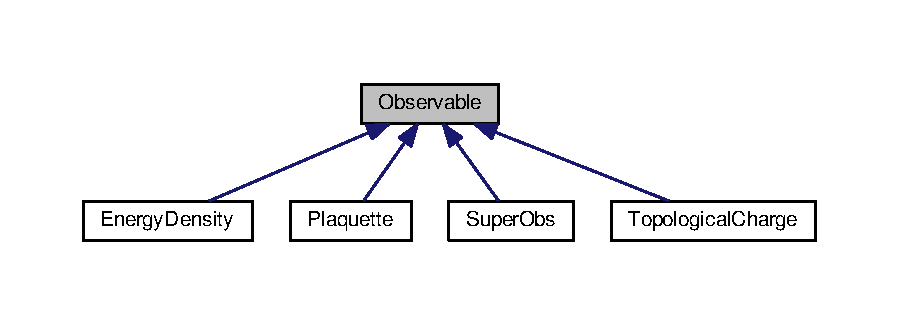
\includegraphics[width=350pt]{classObservable__inherit__graph}
\end{center}
\end{figure}


Collaboration diagram for Observable\+:
\nopagebreak
\begin{figure}[H]
\begin{center}
\leavevmode
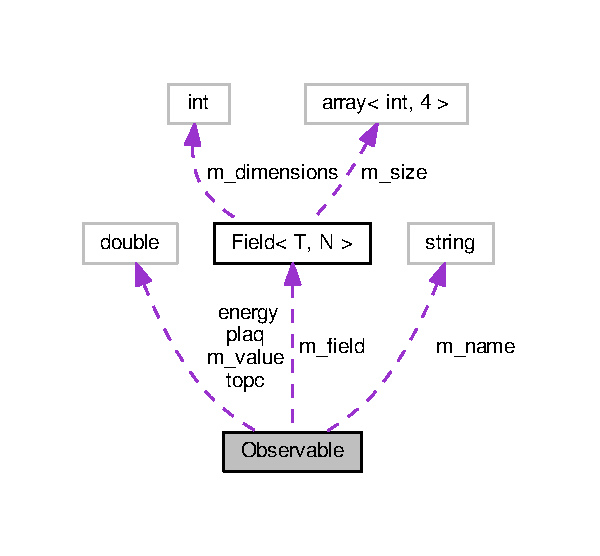
\includegraphics[width=288pt]{classObservable__coll__graph}
\end{center}
\end{figure}
\subsection*{Public Member Functions}
\begin{DoxyCompactItemize}
\item 
virtual void {\bfseries compute} ()=0\hypertarget{classObservable_a3a8881d961623cddb85416cefa1c5432}{}\label{classObservable_a3a8881d961623cddb85416cefa1c5432}

\item 
virtual void {\bfseries init\+Observable} (\hyperlink{classField}{Gluon\+Field} $\ast$field)=0\hypertarget{classObservable_a1baf736c771a8a073554286571be8b09}{}\label{classObservable_a1baf736c771a8a073554286571be8b09}

\item 
const char $\ast$ {\bfseries get\+Name} ()\hypertarget{classObservable_ad3348c3f40782b5e09bc8dbcb8295a79}{}\label{classObservable_ad3348c3f40782b5e09bc8dbcb8295a79}

\item 
double {\bfseries value} ()\hypertarget{classObservable_ab7931d270397e55bfe82384b52db17a0}{}\label{classObservable_ab7931d270397e55bfe82384b52db17a0}

\end{DoxyCompactItemize}
\subsection*{Public Attributes}
\begin{DoxyCompactItemize}
\item 
double {\bfseries plaq}\hypertarget{classObservable_ad9e9bc025babb8fed348d7e16e424ae8}{}\label{classObservable_ad9e9bc025babb8fed348d7e16e424ae8}

\item 
double {\bfseries energy}\hypertarget{classObservable_afe50655b42d350df43ae1fe4ee8cf5fb}{}\label{classObservable_afe50655b42d350df43ae1fe4ee8cf5fb}

\item 
double {\bfseries topc}\hypertarget{classObservable_a18813c913b086462648c9e61d85d6be6}{}\label{classObservable_a18813c913b086462648c9e61d85d6be6}

\end{DoxyCompactItemize}
\subsection*{Protected Member Functions}
\begin{DoxyCompactItemize}
\item 
void {\bfseries gather\+Results} ()\hypertarget{classObservable_ae42f1c4bf6362dde45f8f6e8042f2ff5}{}\label{classObservable_ae42f1c4bf6362dde45f8f6e8042f2ff5}

\end{DoxyCompactItemize}
\subsection*{Protected Attributes}
\begin{DoxyCompactItemize}
\item 
\hyperlink{classField}{Gluon\+Field} $\ast$ {\bfseries m\+\_\+field} = nullptr\hypertarget{classObservable_a3f3b97a6ccf3662fc4285e0249fc7e55}{}\label{classObservable_a3f3b97a6ccf3662fc4285e0249fc7e55}

\item 
double {\bfseries m\+\_\+value}\hypertarget{classObservable_a65689c61e83937902110f9da43b4a327}{}\label{classObservable_a65689c61e83937902110f9da43b4a327}

\item 
std\+::string {\bfseries m\+\_\+name}\hypertarget{classObservable_ac48d8fce3be9fefa7af3bb3cd4e01e06}{}\label{classObservable_ac48d8fce3be9fefa7af3bb3cd4e01e06}

\end{DoxyCompactItemize}


The documentation for this class was generated from the following files\+:\begin{DoxyCompactItemize}
\item 
/home/giovanni/\+Desktop/\+Lattice\+Yang\+Mills/include/\+Observables/observable.\+h\item 
/home/giovanni/\+Desktop/\+Lattice\+Yang\+Mills/src/\+Observables/observable.\+cpp\end{DoxyCompactItemize}

\hypertarget{classLatticeIO_1_1OutputConf}{}\section{Lattice\+IO\+:\+:Output\+Conf Class Reference}
\label{classLatticeIO_1_1OutputConf}\index{Lattice\+I\+O\+::\+Output\+Conf@{Lattice\+I\+O\+::\+Output\+Conf}}
\subsection*{Static Public Member Functions}
\begin{DoxyCompactItemize}
\item 
static void {\bfseries write\+Conf} (\hyperlink{classField}{Gluon\+Field} \&lattice, int conf\+Num)\hypertarget{classLatticeIO_1_1OutputConf_a11ca0a1237c846e35e7fe3aff8dbb4df}{}\label{classLatticeIO_1_1OutputConf_a11ca0a1237c846e35e7fe3aff8dbb4df}

\item 
static void {\bfseries write\+Sub\+Lattice} (\hyperlink{classField}{Gluon\+Field} \&lattice, int conf\+Num)\hypertarget{classLatticeIO_1_1OutputConf_a1c4247249c03a2ec761cf4eee25a47a1}{}\label{classLatticeIO_1_1OutputConf_a1c4247249c03a2ec761cf4eee25a47a1}

\item 
static void {\bfseries set\+Output\+Dir} (std\+::string output\+Dir)\hypertarget{classLatticeIO_1_1OutputConf_a6a14c8a578af927a26a48b01f6fb7907}{}\label{classLatticeIO_1_1OutputConf_a6a14c8a578af927a26a48b01f6fb7907}

\end{DoxyCompactItemize}


The documentation for this class was generated from the following files\+:\begin{DoxyCompactItemize}
\item 
/home/giovanni/\+Desktop/\+Lattice\+Yang\+Mills/include/\+Input\+Output/outputconf.\+h\item 
/home/giovanni/\+Desktop/\+Lattice\+Yang\+Mills/src/\+Input\+Output/outputconf.\+cpp\end{DoxyCompactItemize}

\hypertarget{classLatticeIO_1_1OutputObs}{}\section{Lattice\+IO\+:\+:Output\+Obs Class Reference}
\label{classLatticeIO_1_1OutputObs}\index{Lattice\+I\+O\+::\+Output\+Obs@{Lattice\+I\+O\+::\+Output\+Obs}}


Class for output to file of observables values.  




{\ttfamily \#include $<$outputobs.\+h$>$}



Collaboration diagram for Lattice\+IO\+:\+:Output\+Obs\+:\nopagebreak
\begin{figure}[H]
\begin{center}
\leavevmode
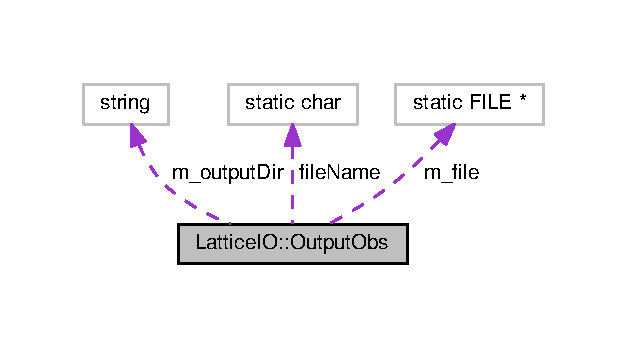
\includegraphics[width=301pt]{dc/d4b/classLatticeIO_1_1OutputObs__coll__graph}
\end{center}
\end{figure}
\subsection*{Static Public Member Functions}
\begin{DoxyCompactItemize}
\item 
static void \hyperlink{classLatticeIO_1_1OutputObs_a472ae3b7d294a80a89642b6464ee8f7d}{initialize} (std\+::vector$<$ \hyperlink{classObservable}{Observable} $\ast$ $>$ \&obs\+List)\hypertarget{classLatticeIO_1_1OutputObs_a472ae3b7d294a80a89642b6464ee8f7d}{}\label{classLatticeIO_1_1OutputObs_a472ae3b7d294a80a89642b6464ee8f7d}

\begin{DoxyCompactList}\small\item\em Opens the files and writes needed headers. \end{DoxyCompactList}\item 
static void \hyperlink{classLatticeIO_1_1OutputObs_a914832abc00b24dc989a3f0b066ff026}{write\+Obs} (std\+::vector$<$ \hyperlink{classObservable}{Observable} $\ast$ $>$ \&obs\+List, int M\+C\+Steps)\hypertarget{classLatticeIO_1_1OutputObs_a914832abc00b24dc989a3f0b066ff026}{}\label{classLatticeIO_1_1OutputObs_a914832abc00b24dc989a3f0b066ff026}

\begin{DoxyCompactList}\small\item\em Writes the list of observables to file at given generation point. \end{DoxyCompactList}\item 
static void \hyperlink{classLatticeIO_1_1OutputObs_a29d0eca3206d892a926ecf051c0ecfc3}{write\+Flow\+Obs} (int conf\+Num, std\+::vector$<$ \hyperlink{classObservable}{Observable} $\ast$ $>$ \&obs\+List, std\+::vector$<$ std\+::vector$<$ double $>$$>$ \&obs\+Matrix)\hypertarget{classLatticeIO_1_1OutputObs_a29d0eca3206d892a926ecf051c0ecfc3}{}\label{classLatticeIO_1_1OutputObs_a29d0eca3206d892a926ecf051c0ecfc3}

\begin{DoxyCompactList}\small\item\em Writes the observables for given flow step. \end{DoxyCompactList}\item 
static void \hyperlink{classLatticeIO_1_1OutputObs_a3adffec5a9f218182a6d45cce7735362}{set\+Output\+Dir} (std\+::string output\+Dir)\hypertarget{classLatticeIO_1_1OutputObs_a3adffec5a9f218182a6d45cce7735362}{}\label{classLatticeIO_1_1OutputObs_a3adffec5a9f218182a6d45cce7735362}

\begin{DoxyCompactList}\small\item\em Sets the output directory for the file output. \end{DoxyCompactList}\end{DoxyCompactItemize}
\subsection*{Static Private Attributes}
\begin{DoxyCompactItemize}
\item 
static F\+I\+LE $\ast$ \hyperlink{classLatticeIO_1_1OutputObs_ad725efe02bfef0f70ef2a43722ce041d}{m\+\_\+file}\hypertarget{classLatticeIO_1_1OutputObs_ad725efe02bfef0f70ef2a43722ce041d}{}\label{classLatticeIO_1_1OutputObs_ad725efe02bfef0f70ef2a43722ce041d}

\begin{DoxyCompactList}\small\item\em The file object for target output. \end{DoxyCompactList}\item 
static char \hyperlink{classLatticeIO_1_1OutputObs_a451f0e835e3dfe2fc70cf779b73aae5d}{file\+Name} \mbox{[}1024\mbox{]}\hypertarget{classLatticeIO_1_1OutputObs_a451f0e835e3dfe2fc70cf779b73aae5d}{}\label{classLatticeIO_1_1OutputObs_a451f0e835e3dfe2fc70cf779b73aae5d}

\begin{DoxyCompactList}\small\item\em The name of the output file. \end{DoxyCompactList}\item 
static std\+::string \hyperlink{classLatticeIO_1_1OutputObs_a3ec9162c9ca9ddae173a1facbaa64a3a}{m\+\_\+output\+Dir}\hypertarget{classLatticeIO_1_1OutputObs_a3ec9162c9ca9ddae173a1facbaa64a3a}{}\label{classLatticeIO_1_1OutputObs_a3ec9162c9ca9ddae173a1facbaa64a3a}

\begin{DoxyCompactList}\small\item\em The output directory. \end{DoxyCompactList}\end{DoxyCompactItemize}


\subsection{Detailed Description}
Class for output to file of observables values. 

\begin{DoxyAuthor}{Author}
Giovanni Pederiva 
\end{DoxyAuthor}
\begin{DoxyVersion}{Version}
1.\+0 
\end{DoxyVersion}
\begin{DoxyDate}{Date}
2017-\/2018 
\end{DoxyDate}
\begin{DoxyCopyright}{Copyright}
M\+IT License.
\end{DoxyCopyright}
This file defines the class needed to file the values of the observables at different steps in the execution. It handles through M\+PI the acces to files depending on rank. Provides output for generation and flow steps. 

The documentation for this class was generated from the following files\+:\begin{DoxyCompactItemize}
\item 
\hyperlink{outputobs_8h}{outputobs.\+h}\item 
outputobs.\+cpp\end{DoxyCompactItemize}

\hypertarget{classLatticeIO_1_1OutputTerm}{}\section{Lattice\+IO\+:\+:Output\+Term Class Reference}
\label{classLatticeIO_1_1OutputTerm}\index{Lattice\+I\+O\+::\+Output\+Term@{Lattice\+I\+O\+::\+Output\+Term}}


Class for standard output.  




{\ttfamily \#include $<$outputterm.\+h$>$}

\subsection*{Static Public Member Functions}
\begin{DoxyCompactItemize}
\item 
static void \hyperlink{classLatticeIO_1_1OutputTerm_ab92340daa2c801b5275d67838df1450b}{print\+Initial\+Conditions} ()
\begin{DoxyCompactList}\small\item\em Prints basic info about the system. \end{DoxyCompactList}\item 
static void \hyperlink{classLatticeIO_1_1OutputTerm_ab06002cace5e0450b9e618edfdb00d12}{write\+Obs} (int conf\+Num, std\+::vector$<$ \hyperlink{classObservable}{Observable} $\ast$ $>$ \&obs\+List)
\begin{DoxyCompactList}\small\item\em Prints the status of the current object list for a given conf. \end{DoxyCompactList}\item 
static void \hyperlink{classLatticeIO_1_1OutputTerm_aecda88f4a7724f1869fb40704d39ef58}{print\+Therm\+Step} (int step, std\+::vector$<$ \hyperlink{classObservable}{Observable} $\ast$ $>$ \&obs\+List, double accept\+Ratio)
\begin{DoxyCompactList}\small\item\em Prints information about a thermalization step. \end{DoxyCompactList}\item 
static void \hyperlink{classLatticeIO_1_1OutputTerm_a82d0d8fc4e4922df3c831c32a6802770}{print\+Gen\+Step} (int conf\+Num, std\+::vector$<$ \hyperlink{classObservable}{Observable} $\ast$ $>$ \&obs\+List, double accept\+Ratio)
\begin{DoxyCompactList}\small\item\em Prints information about a generation step. \end{DoxyCompactList}\item 
static void \hyperlink{classLatticeIO_1_1OutputTerm_a4ba09f68c5cc215b03ca3aec47d76d65}{write\+Flow\+Obs} (double flow\+Time, std\+::vector$<$ \hyperlink{classObservable}{Observable} $\ast$ $>$ \&obs\+List)
\begin{DoxyCompactList}\small\item\em Prints information about a flow time evolution step. \end{DoxyCompactList}\end{DoxyCompactItemize}


\subsection{Detailed Description}
Class for standard output. 

\begin{DoxyAuthor}{Author}
Giovanni Pederiva 
\end{DoxyAuthor}
\begin{DoxyVersion}{Version}
1.\+0 
\end{DoxyVersion}
\begin{DoxyDate}{Date}
2017-\/2018 
\end{DoxyDate}
\begin{DoxyCopyright}{Copyright}
M\+IT License.
\end{DoxyCopyright}
This class handles the standard terminal output dealing with the multi processor nature of the program. It checks on the M\+PI rank in order to decide whether to output or not. It also provides basic tools to print information about the system as it evolves. 

Definition at line 60 of file outputterm.\+h.



\subsection{Member Function Documentation}
\index{Lattice\+I\+O\+::\+Output\+Term@{Lattice\+I\+O\+::\+Output\+Term}!print\+Gen\+Step@{print\+Gen\+Step}}
\index{print\+Gen\+Step@{print\+Gen\+Step}!Lattice\+I\+O\+::\+Output\+Term@{Lattice\+I\+O\+::\+Output\+Term}}
\subsubsection[{\texorpdfstring{print\+Gen\+Step(int conf\+Num, std\+::vector$<$ Observable $\ast$ $>$ \&obs\+List, double accept\+Ratio)}{printGenStep(int confNum, std::vector< Observable * > &obsList, double acceptRatio)}}]{\setlength{\rightskip}{0pt plus 5cm}void Lattice\+I\+O\+::\+Output\+Term\+::print\+Gen\+Step (
\begin{DoxyParamCaption}
\item[{int}]{conf\+Num, }
\item[{std\+::vector$<$ {\bf Observable} $\ast$ $>$ \&}]{obs\+List, }
\item[{double}]{accept\+Ratio}
\end{DoxyParamCaption}
)\hspace{0.3cm}{\ttfamily [static]}}\hypertarget{classLatticeIO_1_1OutputTerm_a82d0d8fc4e4922df3c831c32a6802770}{}\label{classLatticeIO_1_1OutputTerm_a82d0d8fc4e4922df3c831c32a6802770}


Prints information about a generation step. 

print information about the system during the gauge field generation


\begin{DoxyParams}{Parameters}
{\em conf\+Num} & the number of the current configuration that has been generated \\
\hline
{\em obs\+List} & a vector of Observables that will be computed and written to file \\
\hline
{\em accept\+Ratio} & the current acceptance ratio of the Metropolis algorithm \\
\hline
\end{DoxyParams}


Definition at line 77 of file outputterm.\+cpp.

\index{Lattice\+I\+O\+::\+Output\+Term@{Lattice\+I\+O\+::\+Output\+Term}!print\+Initial\+Conditions@{print\+Initial\+Conditions}}
\index{print\+Initial\+Conditions@{print\+Initial\+Conditions}!Lattice\+I\+O\+::\+Output\+Term@{Lattice\+I\+O\+::\+Output\+Term}}
\subsubsection[{\texorpdfstring{print\+Initial\+Conditions()}{printInitialConditions()}}]{\setlength{\rightskip}{0pt plus 5cm}void Lattice\+I\+O\+::\+Output\+Term\+::print\+Initial\+Conditions (
\begin{DoxyParamCaption}
{}
\end{DoxyParamCaption}
)\hspace{0.3cm}{\ttfamily [static]}}\hypertarget{classLatticeIO_1_1OutputTerm_ab92340daa2c801b5275d67838df1450b}{}\label{classLatticeIO_1_1OutputTerm_ab92340daa2c801b5275d67838df1450b}


Prints basic info about the system. 

prints basic information about the system to terminal 

Definition at line 45 of file outputterm.\+cpp.

\index{Lattice\+I\+O\+::\+Output\+Term@{Lattice\+I\+O\+::\+Output\+Term}!print\+Therm\+Step@{print\+Therm\+Step}}
\index{print\+Therm\+Step@{print\+Therm\+Step}!Lattice\+I\+O\+::\+Output\+Term@{Lattice\+I\+O\+::\+Output\+Term}}
\subsubsection[{\texorpdfstring{print\+Therm\+Step(int step, std\+::vector$<$ Observable $\ast$ $>$ \&obs\+List, double accept\+Ratio)}{printThermStep(int step, std::vector< Observable * > &obsList, double acceptRatio)}}]{\setlength{\rightskip}{0pt plus 5cm}void Lattice\+I\+O\+::\+Output\+Term\+::print\+Therm\+Step (
\begin{DoxyParamCaption}
\item[{int}]{step, }
\item[{std\+::vector$<$ {\bf Observable} $\ast$ $>$ \&}]{obs\+List, }
\item[{double}]{accept\+Ratio}
\end{DoxyParamCaption}
)\hspace{0.3cm}{\ttfamily [static]}}\hypertarget{classLatticeIO_1_1OutputTerm_aecda88f4a7724f1869fb40704d39ef58}{}\label{classLatticeIO_1_1OutputTerm_aecda88f4a7724f1869fb40704d39ef58}


Prints information about a thermalization step. 

print information about the system during thermalization


\begin{DoxyParams}{Parameters}
{\em step} & the curren thermalization step \\
\hline
{\em obs\+List} & a vector of Observables that will be computed and written to file \\
\hline
{\em accept\+Ratio} & the current acceptance ratio of the Metropolis algorithm \\
\hline
\end{DoxyParams}


Definition at line 62 of file outputterm.\+cpp.

\index{Lattice\+I\+O\+::\+Output\+Term@{Lattice\+I\+O\+::\+Output\+Term}!write\+Flow\+Obs@{write\+Flow\+Obs}}
\index{write\+Flow\+Obs@{write\+Flow\+Obs}!Lattice\+I\+O\+::\+Output\+Term@{Lattice\+I\+O\+::\+Output\+Term}}
\subsubsection[{\texorpdfstring{write\+Flow\+Obs(double flow\+Time, std\+::vector$<$ Observable $\ast$ $>$ \&obs\+List)}{writeFlowObs(double flowTime, std::vector< Observable * > &obsList)}}]{\setlength{\rightskip}{0pt plus 5cm}void Lattice\+I\+O\+::\+Output\+Term\+::write\+Flow\+Obs (
\begin{DoxyParamCaption}
\item[{double}]{flow\+Time, }
\item[{std\+::vector$<$ {\bf Observable} $\ast$ $>$ \&}]{obs\+List}
\end{DoxyParamCaption}
)\hspace{0.3cm}{\ttfamily [static]}}\hypertarget{classLatticeIO_1_1OutputTerm_a4ba09f68c5cc215b03ca3aec47d76d65}{}\label{classLatticeIO_1_1OutputTerm_a4ba09f68c5cc215b03ca3aec47d76d65}


Prints information about a flow time evolution step. 

print information about the system during the gradient flow steps


\begin{DoxyParams}{Parameters}
{\em flow\+Time} & the current flow time of the integration \\
\hline
{\em obs\+List} & a vector of Observables that will be computed and written to file \\
\hline
\end{DoxyParams}


Definition at line 108 of file outputterm.\+cpp.

\index{Lattice\+I\+O\+::\+Output\+Term@{Lattice\+I\+O\+::\+Output\+Term}!write\+Obs@{write\+Obs}}
\index{write\+Obs@{write\+Obs}!Lattice\+I\+O\+::\+Output\+Term@{Lattice\+I\+O\+::\+Output\+Term}}
\subsubsection[{\texorpdfstring{write\+Obs(int conf\+Num, std\+::vector$<$ Observable $\ast$ $>$ \&obs\+List)}{writeObs(int confNum, std::vector< Observable * > &obsList)}}]{\setlength{\rightskip}{0pt plus 5cm}void Lattice\+I\+O\+::\+Output\+Term\+::write\+Obs (
\begin{DoxyParamCaption}
\item[{int}]{conf\+Num, }
\item[{std\+::vector$<$ {\bf Observable} $\ast$ $>$ \&}]{obs\+List}
\end{DoxyParamCaption}
)\hspace{0.3cm}{\ttfamily [static]}}\hypertarget{classLatticeIO_1_1OutputTerm_ab06002cace5e0450b9e618edfdb00d12}{}\label{classLatticeIO_1_1OutputTerm_ab06002cace5e0450b9e618edfdb00d12}


Prints the status of the current object list for a given conf. 

print information about the system of a given configuration


\begin{DoxyParams}{Parameters}
{\em conf\+Num} & the number of the current configuration \\
\hline
{\em obs\+List} & a vector of Observables that will be computed and written to file \\
\hline
\end{DoxyParams}


Definition at line 91 of file outputterm.\+cpp.



The documentation for this class was generated from the following files\+:\begin{DoxyCompactItemize}
\item 
\hyperlink{outputterm_8h}{outputterm.\+h}\item 
\hyperlink{outputterm_8cpp}{outputterm.\+cpp}\end{DoxyCompactItemize}

\hypertarget{classParallel}{}\section{Parallel Class Reference}
\label{classParallel}\index{Parallel@{Parallel}}
\subsection*{Static Public Member Functions}
\begin{DoxyCompactItemize}
\item 
static void {\bfseries initialize} ()\hypertarget{classParallel_a7cf27d593972dee2d3f6e5319fcf450e}{}\label{classParallel_a7cf27d593972dee2d3f6e5319fcf450e}

\item 
static void {\bfseries create\+Geometry} (std\+::array$<$ int, 4 $>$ lattice\+Size, std\+::array$<$ int, 4 $>$ sub\+Lattice\+Size)\hypertarget{classParallel_a8888fe404de3a3f479fff0796916f851}{}\label{classParallel_a8888fe404de3a3f479fff0796916f851}

\item 
static void {\bfseries finalize} ()\hypertarget{classParallel_ac81d8fad81830939d9338b2e46d71b60}{}\label{classParallel_ac81d8fad81830939d9338b2e46d71b60}

\item 
static int {\bfseries rank} ()\hypertarget{classParallel_ad8a436ba61d28a6f7569eec3ac4a929e}{}\label{classParallel_ad8a436ba61d28a6f7569eec3ac4a929e}

\item 
static int {\bfseries num\+Procs} ()\hypertarget{classParallel_a6af0b709a019dd91b0d3bbd4a2b74e54}{}\label{classParallel_a6af0b709a019dd91b0d3bbd4a2b74e54}

\item 
static int {\bfseries active\+Procs} ()\hypertarget{classParallel_a9569b920d302407a51a43c125a878b43}{}\label{classParallel_a9569b920d302407a51a43c125a878b43}

\item 
static bool {\bfseries is\+Active} ()\hypertarget{classParallel_a1402031c4027212fa9cd53cbe86b5b41}{}\label{classParallel_a1402031c4027212fa9cd53cbe86b5b41}

\item 
static M\+P\+I\+\_\+\+Comm {\bfseries cart\+Coord\+Comm} ()\hypertarget{classParallel_a127b363a07b22186627f532b2ab04c28}{}\label{classParallel_a127b363a07b22186627f532b2ab04c28}

\item 
static std\+::array$<$ int, 4 $>$ \& {\bfseries sub\+Blocks} ()\hypertarget{classParallel_ad237dc02b7a88cfc454b5a87573588ea}{}\label{classParallel_ad237dc02b7a88cfc454b5a87573588ea}

\item 
static std\+::array$<$ int, 4 $>$ \& {\bfseries rank\+Coord} ()\hypertarget{classParallel_a64dc2b62abe04ae4eeb2c55f9407b9dd}{}\label{classParallel_a64dc2b62abe04ae4eeb2c55f9407b9dd}

\item 
static std\+::array$<$ int, 4 $>$ \& {\bfseries lattice\+Sub\+Size} ()\hypertarget{classParallel_addeb93b221ca944c1916033f8ac5144e}{}\label{classParallel_addeb93b221ca944c1916033f8ac5144e}

\item 
static std\+::array$<$ int, 4 $>$ \& {\bfseries lattice\+Full\+Size} ()\hypertarget{classParallel_a5e2b7f890813ffc45221d92aee3e51bd}{}\label{classParallel_a5e2b7f890813ffc45221d92aee3e51bd}

\item 
static std\+::array$<$ int, 4 $>$ \& {\bfseries parity} ()\hypertarget{classParallel_ae4d683542868851b8d8229493c0fa412}{}\label{classParallel_ae4d683542868851b8d8229493c0fa412}

\item 
static int {\bfseries get\+Neighbor} (int direction, int sign)\hypertarget{classParallel_a4e99d3605b17fb51fa8a566cf0730179}{}\label{classParallel_a4e99d3605b17fb51fa8a566cf0730179}

\item 
static int {\bfseries get\+Second\+Neighbor} (int direction1, int sign1, int direction2, int sign2)\hypertarget{classParallel_afaecf8622c16bb5def671d881821db7d}{}\label{classParallel_afaecf8622c16bb5def671d881821db7d}

\item 
static void {\bfseries open\+File} (M\+P\+I\+\_\+\+File \&file, const char $\ast$file\+Name)\hypertarget{classParallel_afea26fc4854070b69224b42962b13091}{}\label{classParallel_afea26fc4854070b69224b42962b13091}

\item 
static void {\bfseries close\+File} (M\+P\+I\+\_\+\+File \&file)\hypertarget{classParallel_ad9ace91bf01fd00c19f7a20efc796285}{}\label{classParallel_ad9ace91bf01fd00c19f7a20efc796285}

\end{DoxyCompactItemize}


The documentation for this class was generated from the following files\+:\begin{DoxyCompactItemize}
\item 
/home/giovanni/\+Desktop/\+Lattice\+Yang\+Mills/include/\+Parallel\+Tools/parallel.\+h\item 
/home/giovanni/\+Desktop/\+Lattice\+Yang\+Mills/src/\+Parallel\+Tools/parallel.\+cpp\end{DoxyCompactItemize}

\hypertarget{classPlaquette}{}\section{Plaquette Class Reference}
\label{classPlaquette}\index{Plaquette@{Plaquette}}


Inheritance diagram for Plaquette\+:\nopagebreak
\begin{figure}[H]
\begin{center}
\leavevmode
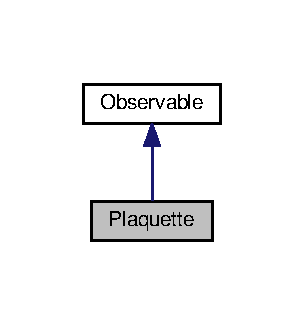
\includegraphics[width=146pt]{db/d05/classPlaquette__inherit__graph}
\end{center}
\end{figure}


Collaboration diagram for Plaquette\+:\nopagebreak
\begin{figure}[H]
\begin{center}
\leavevmode
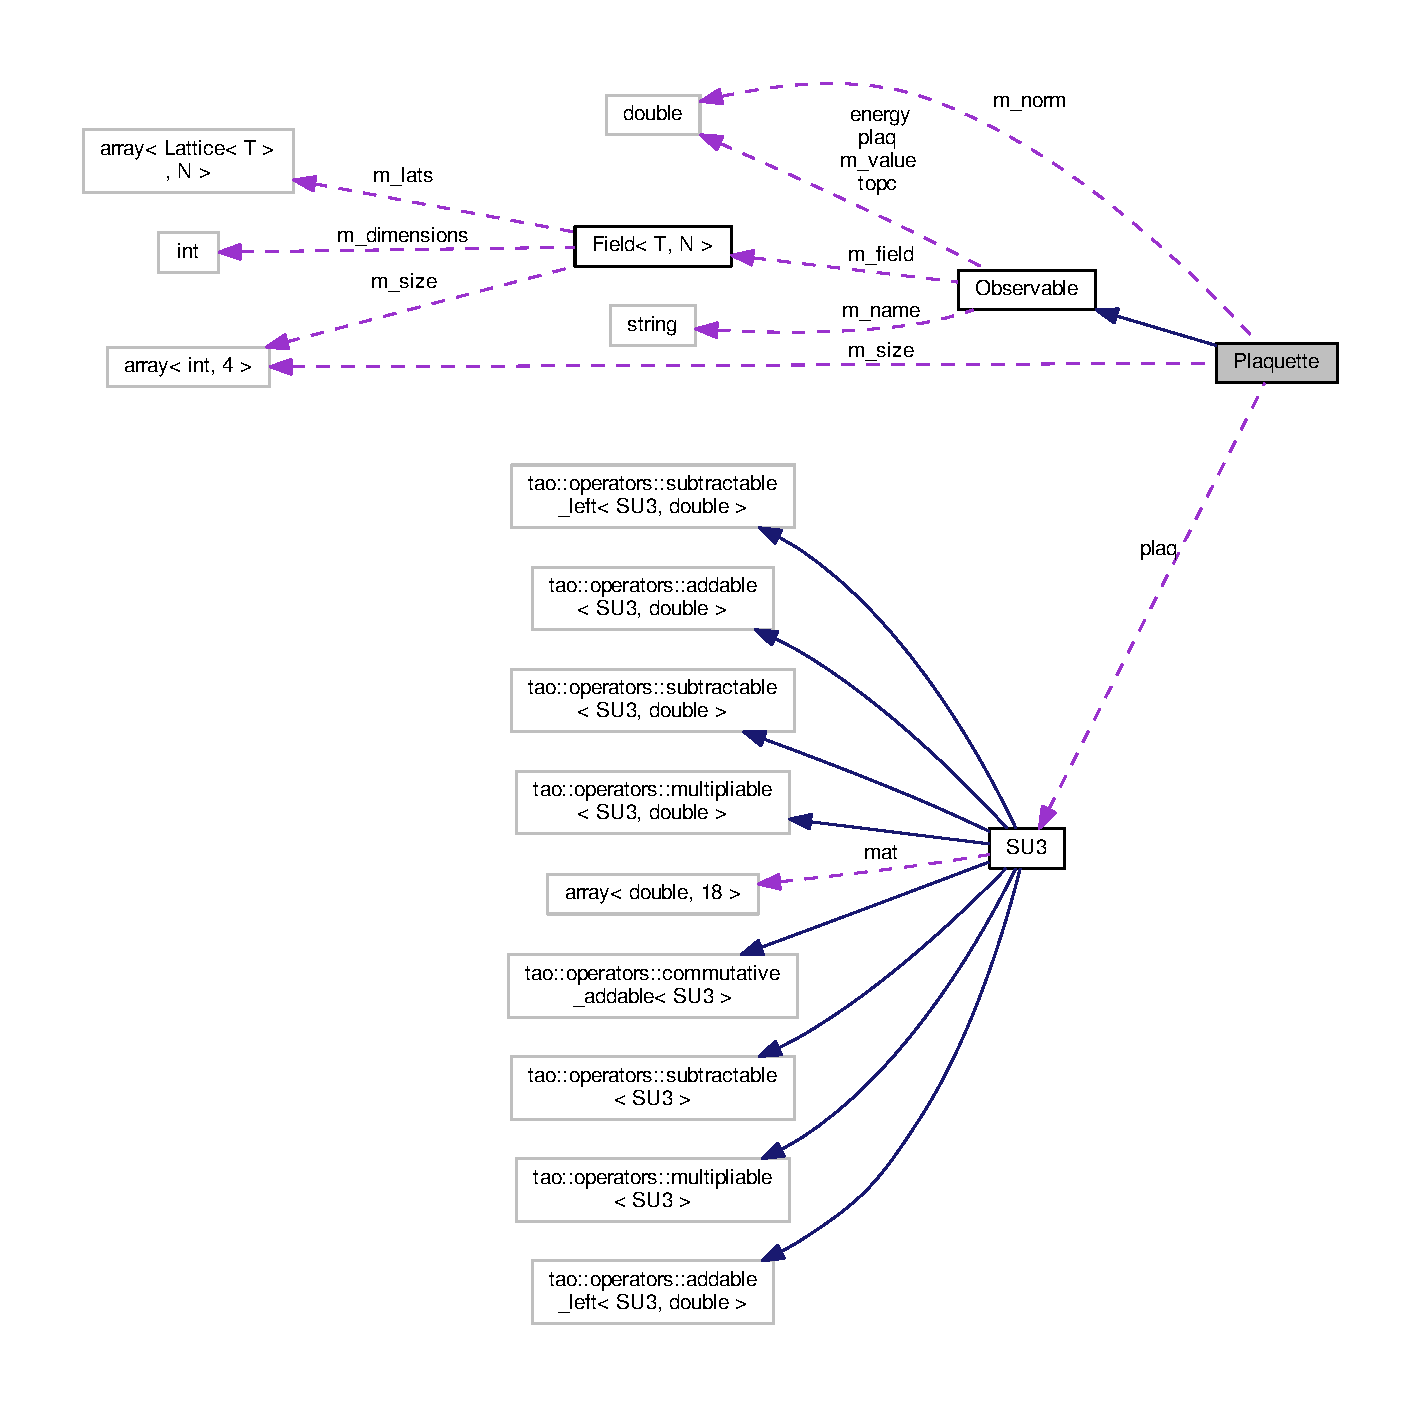
\includegraphics[width=350pt]{d0/d3a/classPlaquette__coll__graph}
\end{center}
\end{figure}
\subsection*{Public Member Functions}
\begin{DoxyCompactItemize}
\item 
void {\bfseries init\+Observable} (\hyperlink{classLattice}{Lattice} $\ast$lattice)\hypertarget{classPlaquette_a736815cd93211ae6762d26f3694a88d5}{}\label{classPlaquette_a736815cd93211ae6762d26f3694a88d5}

\item 
void {\bfseries compute} ()\hypertarget{classPlaquette_a4f5cd3222dc5ecec563ff873507493ea}{}\label{classPlaquette_a4f5cd3222dc5ecec563ff873507493ea}

\end{DoxyCompactItemize}
\subsection*{Private Attributes}
\begin{DoxyCompactItemize}
\item 
std\+::array$<$ int, 4 $>$ {\bfseries m\+\_\+size}\hypertarget{classPlaquette_aef320da834a652eef5dc9fdaf9feb898}{}\label{classPlaquette_aef320da834a652eef5dc9fdaf9feb898}

\item 
double {\bfseries m\+\_\+norm}\hypertarget{classPlaquette_a01a530c15a05f0d0c0db0ee96df7f943}{}\label{classPlaquette_a01a530c15a05f0d0c0db0ee96df7f943}

\item 
\hyperlink{structSU3}{S\+U3} {\bfseries plaq}\hypertarget{classPlaquette_ada0642da7642a9d271681985b93a4070}{}\label{classPlaquette_ada0642da7642a9d271681985b93a4070}

\end{DoxyCompactItemize}
\subsection*{Additional Inherited Members}


The documentation for this class was generated from the following files\+:\begin{DoxyCompactItemize}
\item 
plaquette.\+h\item 
plaquette.\+cpp\end{DoxyCompactItemize}

\hypertarget{classPureGauge}{}\section{Pure\+Gauge Class Reference}
\label{classPureGauge}\index{Pure\+Gauge@{Pure\+Gauge}}


Implementation of the \hyperlink{classPureGauge}{Pure\+Gauge} derived \hyperlink{classAction}{Action} class.  




{\ttfamily \#include $<$puregauge.\+h$>$}



Inheritance diagram for Pure\+Gauge\+:\nopagebreak
\begin{figure}[H]
\begin{center}
\leavevmode
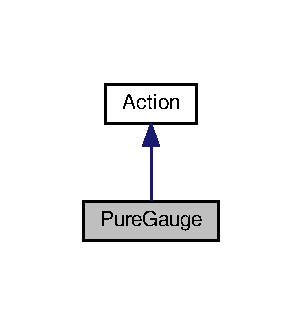
\includegraphics[width=145pt]{d8/da5/classPureGauge__inherit__graph}
\end{center}
\end{figure}


Collaboration diagram for Pure\+Gauge\+:\nopagebreak
\begin{figure}[H]
\begin{center}
\leavevmode
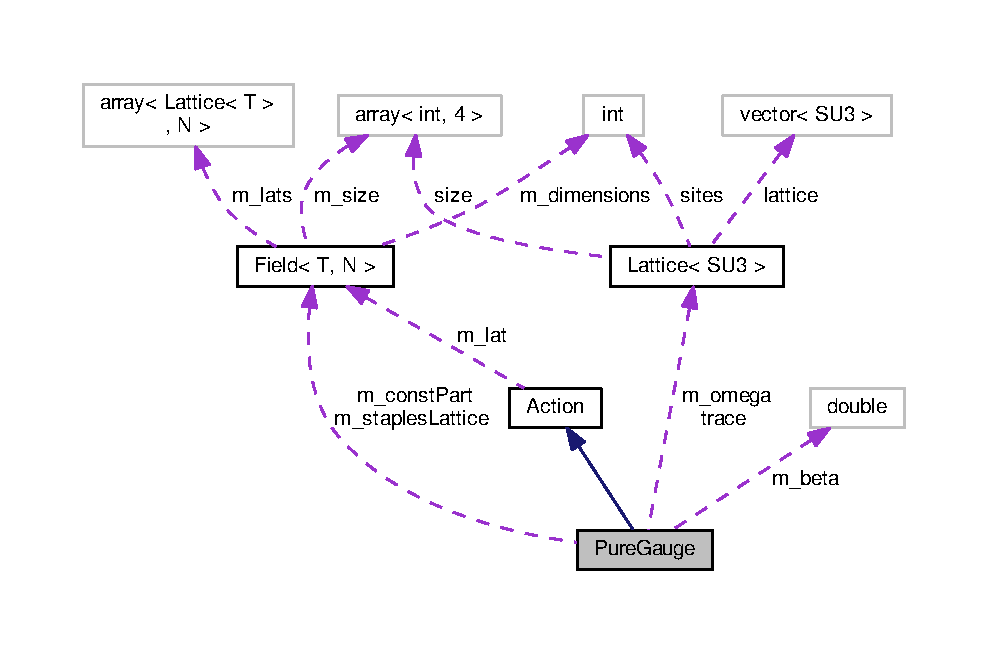
\includegraphics[width=350pt]{da/d42/classPureGauge__coll__graph}
\end{center}
\end{figure}
\subsection*{Public Member Functions}
\begin{DoxyCompactItemize}
\item 
{\bfseries Pure\+Gauge} (\hyperlink{field_8h_afe80b127697eba6d6e7fbd8121c8d4ee}{Gluon\+Field} $\ast$lattice, double beta)\hypertarget{classPureGauge_ae832fd1e6b53f6ca3d22961f4a2f80f7}{}\label{classPureGauge_ae832fd1e6b53f6ca3d22961f4a2f80f7}

\item 
\hyperlink{classPureGauge_ab219e717e036ee44696ba360a2b3674b}{Pure\+Gauge} (double beta)
\begin{DoxyCompactList}\small\item\em Initializer for the \hyperlink{classPureGauge}{Pure\+Gauge} \hyperlink{classAction}{Action} class. \end{DoxyCompactList}\item 
double \hyperlink{classPureGauge_a17facfc54c75a588826c00f8ef185bf0}{compute} (int x, int y, int z, int t, int mu, \hyperlink{structSU3}{S\+U3} \&new\+Link)\hypertarget{classPureGauge_a17facfc54c75a588826c00f8ef185bf0}{}\label{classPureGauge_a17facfc54c75a588826c00f8ef185bf0}

\begin{DoxyCompactList}\small\item\em Computes the action difference around a given link for a suggested move. \end{DoxyCompactList}\item 
void \hyperlink{classPureGauge_a7c78eb206450a209b4154fc936d8aad1}{compute\+Staples} (int mu)
\begin{DoxyCompactList}\small\item\em Computes the staples along the given directionfor all links in the given direction. \end{DoxyCompactList}\item 
\hyperlink{classLattice}{Lattice}$<$ \hyperlink{structSU3}{S\+U3} $>$ \hyperlink{classPureGauge_a0d9272be98cf62567bbda93a892718eb}{compute\+Derivative} (int mu)
\begin{DoxyCompactList}\small\item\em Computes the derivative of all links along the given direction. \end{DoxyCompactList}\item 
void {\bfseries compute\+Staplez} (\hyperlink{field_8h_afe80b127697eba6d6e7fbd8121c8d4ee}{Gluon\+Field} $\ast$lattice)\hypertarget{classPureGauge_a28706ff95422d3ac6e1dc9d2aabccf1a}{}\label{classPureGauge_a28706ff95422d3ac6e1dc9d2aabccf1a}

\item 
void {\bfseries compute\+Other\+Staples} (int x, int y, int z, int t, int mu)\hypertarget{classPureGauge_a5722f484c169539471da120aefa97dea}{}\label{classPureGauge_a5722f484c169539471da120aefa97dea}

\end{DoxyCompactItemize}
\subsection*{Private Attributes}
\begin{DoxyCompactItemize}
\item 
double {\bfseries m\+\_\+beta}\hypertarget{classPureGauge_afc5d5fd50c90502b1851f7fa7295e68d}{}\label{classPureGauge_afc5d5fd50c90502b1851f7fa7295e68d}

\item 
\hyperlink{field_8h_afe80b127697eba6d6e7fbd8121c8d4ee}{Gluon\+Field} $\ast$ {\bfseries m\+\_\+staples\+Lattice} = nullptr\hypertarget{classPureGauge_ae2b14c7d0c1e2f5cb070b9d8ed9ab237}{}\label{classPureGauge_ae2b14c7d0c1e2f5cb070b9d8ed9ab237}

\item 
\hyperlink{field_8h_afe80b127697eba6d6e7fbd8121c8d4ee}{Gluon\+Field} $\ast$ {\bfseries m\+\_\+const\+Part}\hypertarget{classPureGauge_ae120c791a7462c26995eebc902a2ae2a}{}\label{classPureGauge_ae120c791a7462c26995eebc902a2ae2a}

\item 
\hyperlink{classLattice}{Lattice}$<$ \hyperlink{structSU3}{S\+U3} $>$ {\bfseries m\+\_\+omega}\hypertarget{classPureGauge_a1a70fe500b7f005c0e82da6b7c5f3509}{}\label{classPureGauge_a1a70fe500b7f005c0e82da6b7c5f3509}

\item 
\hyperlink{classLattice}{Lattice}$<$ \hyperlink{structSU3}{S\+U3} $>$ {\bfseries trace}\hypertarget{classPureGauge_abbe94c552df9ba24ba63377189af9f24}{}\label{classPureGauge_abbe94c552df9ba24ba63377189af9f24}

\end{DoxyCompactItemize}
\subsection*{Additional Inherited Members}


\subsection{Detailed Description}
Implementation of the \hyperlink{classPureGauge}{Pure\+Gauge} derived \hyperlink{classAction}{Action} class. 

\begin{DoxyAuthor}{Author}
Giovanni Pederiva 
\end{DoxyAuthor}
\begin{DoxyVersion}{Version}
1.\+0 
\end{DoxyVersion}
\begin{DoxyDate}{Date}
2017-\/2018 
\end{DoxyDate}
\begin{DoxyCopyright}{Copyright}
M\+IT License.
\end{DoxyCopyright}
The \hyperlink{classPureGauge}{Pure\+Gauge} class implements the Wilson \hyperlink{classPlaquette}{Plaquette} \hyperlink{classAction}{Action} in its simplest formulation. The action is given by the sum of the plaquettes around a specified link. 

Definition at line 50 of file puregauge.\+h.



\subsection{Constructor \& Destructor Documentation}
\index{Pure\+Gauge@{Pure\+Gauge}!Pure\+Gauge@{Pure\+Gauge}}
\index{Pure\+Gauge@{Pure\+Gauge}!Pure\+Gauge@{Pure\+Gauge}}
\subsubsection[{\texorpdfstring{Pure\+Gauge(double beta)}{PureGauge(double beta)}}]{\setlength{\rightskip}{0pt plus 5cm}Pure\+Gauge\+::\+Pure\+Gauge (
\begin{DoxyParamCaption}
\item[{double}]{beta}
\end{DoxyParamCaption}
)}\hypertarget{classPureGauge_ab219e717e036ee44696ba360a2b3674b}{}\label{classPureGauge_ab219e717e036ee44696ba360a2b3674b}


Initializer for the \hyperlink{classPureGauge}{Pure\+Gauge} \hyperlink{classAction}{Action} class. 


\begin{DoxyParams}{Parameters}
{\em beta} & The \$/beta\$ value of the action \\
\hline
\end{DoxyParams}


Definition at line 50 of file puregauge.\+cpp.



\subsection{Member Function Documentation}
\index{Pure\+Gauge@{Pure\+Gauge}!compute\+Derivative@{compute\+Derivative}}
\index{compute\+Derivative@{compute\+Derivative}!Pure\+Gauge@{Pure\+Gauge}}
\subsubsection[{\texorpdfstring{compute\+Derivative(int mu)}{computeDerivative(int mu)}}]{\setlength{\rightskip}{0pt plus 5cm}{\bf Lattice}$<$ {\bf S\+U3} $>$ Pure\+Gauge\+::compute\+Derivative (
\begin{DoxyParamCaption}
\item[{int}]{mu}
\end{DoxyParamCaption}
)\hspace{0.3cm}{\ttfamily [virtual]}}\hypertarget{classPureGauge_a0d9272be98cf62567bbda93a892718eb}{}\label{classPureGauge_a0d9272be98cf62567bbda93a892718eb}


Computes the derivative of all links along the given direction. 


\begin{DoxyParams}{Parameters}
{\em mu} & The index of the directions to compute the staples of \\
\hline
\end{DoxyParams}
\begin{DoxyReturn}{Returns}
m\+\_\+omega \hyperlink{classLattice}{Lattice$<$\+S\+U3$>$} containing the derivative of the Gluon\+Field 
\end{DoxyReturn}


Implements \hyperlink{classAction_a722e4f88dda82440d0c6e19a43972b21}{Action}.



Definition at line 94 of file puregauge.\+cpp.

\index{Pure\+Gauge@{Pure\+Gauge}!compute\+Staples@{compute\+Staples}}
\index{compute\+Staples@{compute\+Staples}!Pure\+Gauge@{Pure\+Gauge}}
\subsubsection[{\texorpdfstring{compute\+Staples(int mu)}{computeStaples(int mu)}}]{\setlength{\rightskip}{0pt plus 5cm}void Pure\+Gauge\+::compute\+Staples (
\begin{DoxyParamCaption}
\item[{int}]{mu}
\end{DoxyParamCaption}
)\hspace{0.3cm}{\ttfamily [virtual]}}\hypertarget{classPureGauge_a7c78eb206450a209b4154fc936d8aad1}{}\label{classPureGauge_a7c78eb206450a209b4154fc936d8aad1}


Computes the staples along the given directionfor all links in the given direction. 


\begin{DoxyParams}{Parameters}
{\em mu} & The index of the directions to compute the staples of \\
\hline
\end{DoxyParams}


Implements \hyperlink{classAction_ad6c5003169695d5cba0f69580040db50}{Action}.



Definition at line 68 of file puregauge.\+cpp.



The documentation for this class was generated from the following files\+:\begin{DoxyCompactItemize}
\item 
\hyperlink{puregauge_8h}{puregauge.\+h}\item 
\hyperlink{puregauge_8cpp}{puregauge.\+cpp}\end{DoxyCompactItemize}

\hypertarget{classRandom}{}\section{Random Class Reference}
\label{classRandom}\index{Random@{Random}}
\subsection*{Static Public Member Functions}
\begin{DoxyCompactItemize}
\item 
static double {\bfseries rand\+Uniform} ()\hypertarget{classRandom_a85d1fc4b7dd6a2a659c02101a87f7a46}{}\label{classRandom_a85d1fc4b7dd6a2a659c02101a87f7a46}

\item 
static \hyperlink{structSU3}{S\+U3} {\bfseries rand\+S\+U3} ()\hypertarget{classRandom_ac5292fc838c1321ef8657947456a3970}{}\label{classRandom_ac5292fc838c1321ef8657947456a3970}

\item 
static \hyperlink{structSU3}{S\+U3} {\bfseries rand\+S\+U3\+Transf} (double epsilon)\hypertarget{classRandom_a1999be7abe21383e442a5ef96fe836f4}{}\label{classRandom_a1999be7abe21383e442a5ef96fe836f4}

\end{DoxyCompactItemize}


The documentation for this class was generated from the following files\+:\begin{DoxyCompactItemize}
\item 
/home/giovanni/\+Desktop/\+Lattice\+Yang\+Mills/include/\+Math/random.\+h\item 
/home/giovanni/\+Desktop/\+Lattice\+Yang\+Mills/src/\+Math/random.\+cpp\end{DoxyCompactItemize}

\hypertarget{structSU3}{}\section{S\+U3 Struct Reference}
\label{structSU3}\index{S\+U3@{S\+U3}}


Inheritance diagram for S\+U3\+:
\nopagebreak
\begin{figure}[H]
\begin{center}
\leavevmode
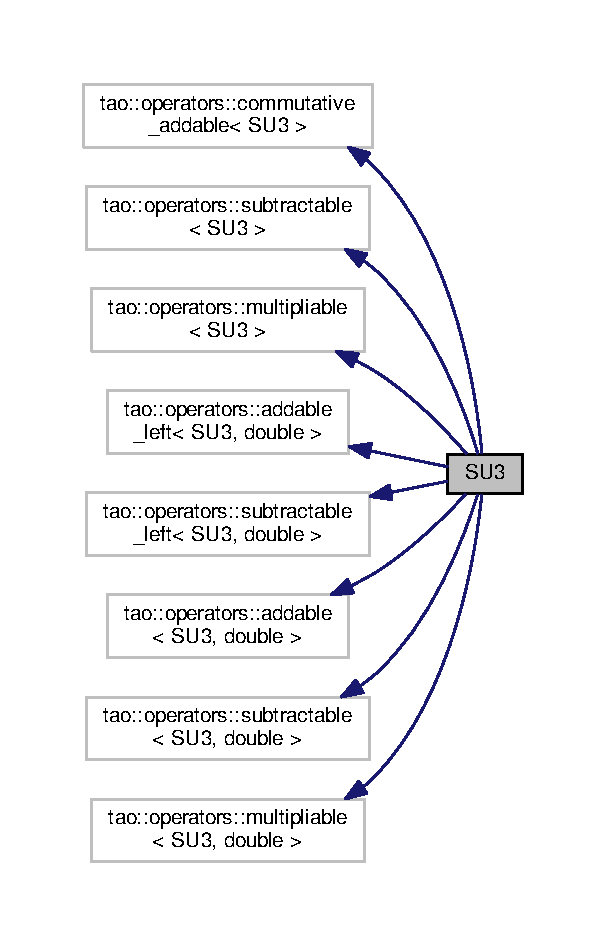
\includegraphics[width=291pt]{structSU3__inherit__graph}
\end{center}
\end{figure}


Collaboration diagram for S\+U3\+:
\nopagebreak
\begin{figure}[H]
\begin{center}
\leavevmode
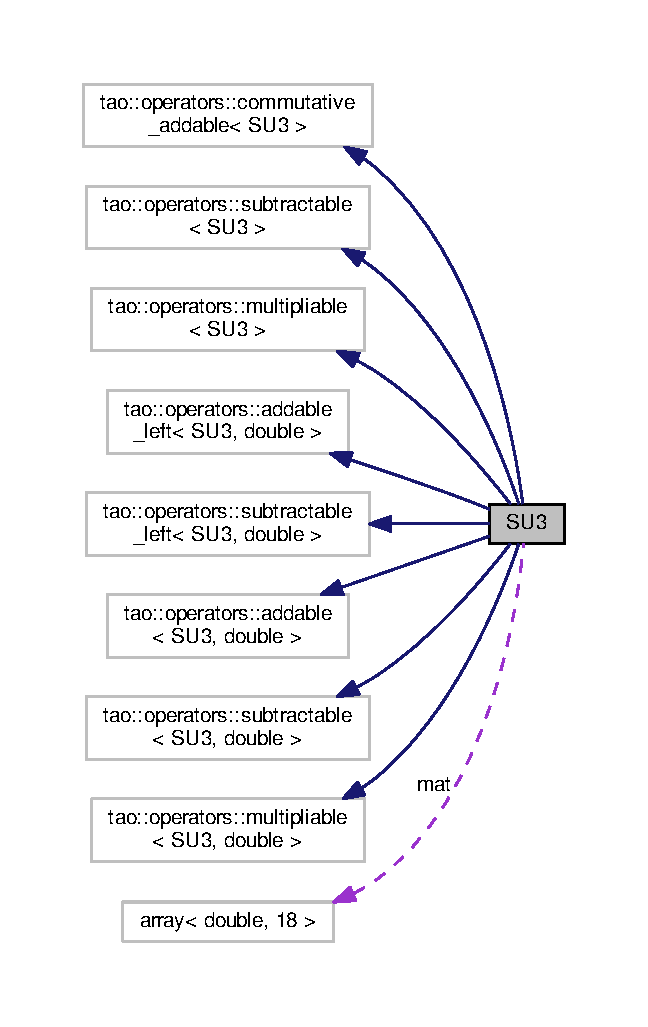
\includegraphics[width=311pt]{structSU3__coll__graph}
\end{center}
\end{figure}
\subsection*{Public Member Functions}
\begin{DoxyCompactItemize}
\item 
{\bfseries S\+U3} (double value) noexcept\hypertarget{structSU3_a15946478b359476373404300768a0cfc}{}\label{structSU3_a15946478b359476373404300768a0cfc}

\item 
{\bfseries S\+U3} (const \hyperlink{structSU3}{S\+U3} \&source) noexcept\hypertarget{structSU3_a622bffa0da5f1b3970d693fcd223cc3c}{}\label{structSU3_a622bffa0da5f1b3970d693fcd223cc3c}

\item 
{\bfseries S\+U3} (\hyperlink{structSU3}{S\+U3} \&\&source) noexcept\hypertarget{structSU3_aa8803a4e0fe94741b8b19a11e7fd4f59}{}\label{structSU3_aa8803a4e0fe94741b8b19a11e7fd4f59}

\item 
\hyperlink{structSU3}{S\+U3} \& {\bfseries operator=} (const \hyperlink{structSU3}{S\+U3} \&other) noexcept\hypertarget{structSU3_a8cba1351e42d60515e99391878012e08}{}\label{structSU3_a8cba1351e42d60515e99391878012e08}

\item 
\hyperlink{structSU3}{S\+U3} \& {\bfseries operator=} (\hyperlink{structSU3}{S\+U3} \&\&other) noexcept\hypertarget{structSU3_ae691a930d90c9247dfdd1538826b0e86}{}\label{structSU3_ae691a930d90c9247dfdd1538826b0e86}

\item 
\hyperlink{structSU3}{S\+U3} \& {\bfseries operator+=} (const \hyperlink{structSU3}{S\+U3} \&other) noexcept\hypertarget{structSU3_a4534185b8910bddd672dd2686613e5cd}{}\label{structSU3_a4534185b8910bddd672dd2686613e5cd}

\item 
\hyperlink{structSU3}{S\+U3} \& {\bfseries operator+=} (\hyperlink{structSU3}{S\+U3} \&\&other) noexcept\hypertarget{structSU3_ae9ecdb599a8afee35a4044c17424a15a}{}\label{structSU3_ae9ecdb599a8afee35a4044c17424a15a}

\item 
\hyperlink{structSU3}{S\+U3} \& {\bfseries operator-\/=} (const \hyperlink{structSU3}{S\+U3} \&other) noexcept\hypertarget{structSU3_a1e95abef99c6d8e02ab9e1b939c98b7d}{}\label{structSU3_a1e95abef99c6d8e02ab9e1b939c98b7d}

\item 
\hyperlink{structSU3}{S\+U3} \& {\bfseries operator-\/=} (\hyperlink{structSU3}{S\+U3} \&\&other) noexcept\hypertarget{structSU3_af6e733c2d12e42c56d8f441af82f2175}{}\label{structSU3_af6e733c2d12e42c56d8f441af82f2175}

\item 
\hyperlink{structSU3}{S\+U3} \& {\bfseries operator$\ast$=} (const \hyperlink{structSU3}{S\+U3} \&other) noexcept\hypertarget{structSU3_a2ca989886022b9c4ce648c30ffbfc00d}{}\label{structSU3_a2ca989886022b9c4ce648c30ffbfc00d}

\item 
\hyperlink{structSU3}{S\+U3} \& {\bfseries operator$\ast$=} (\hyperlink{structSU3}{S\+U3} \&\&other) noexcept\hypertarget{structSU3_a12618dbf115cbee343984b4b4948d665}{}\label{structSU3_a12618dbf115cbee343984b4b4948d665}

\item 
\hyperlink{structSU3}{S\+U3} \& {\bfseries operator+=} (const double scalar) noexcept\hypertarget{structSU3_a263c356674752425cd4a11f76bb8fc36}{}\label{structSU3_a263c356674752425cd4a11f76bb8fc36}

\item 
\hyperlink{structSU3}{S\+U3} \& {\bfseries operator-\/=} (const double scalar) noexcept\hypertarget{structSU3_a8fd821cd749e0f69bd64e63fc1a48b84}{}\label{structSU3_a8fd821cd749e0f69bd64e63fc1a48b84}

\item 
\hyperlink{structSU3}{S\+U3} \& {\bfseries operator$\ast$=} (const double scalar) noexcept\hypertarget{structSU3_a36a3ff37fa53ad0f2650cbcaebeceb94}{}\label{structSU3_a36a3ff37fa53ad0f2650cbcaebeceb94}

\item 
void {\bfseries set\+S\+U3\+Identity} ()\hypertarget{structSU3_a7dc0fede260d68f5967782dde7e3390e}{}\label{structSU3_a7dc0fede260d68f5967782dde7e3390e}

\item 
void {\bfseries set\+S\+U3\+Zero} ()\hypertarget{structSU3_a97e16430a059521473daf753e68cc671}{}\label{structSU3_a97e16430a059521473daf753e68cc671}

\item 
void {\bfseries set\+S\+U3\+Random} ()\hypertarget{structSU3_aeb586c42202c0a418d0212c5c715b42d}{}\label{structSU3_aeb586c42202c0a418d0212c5c715b42d}

\item 
double {\bfseries real\+Trace} ()\hypertarget{structSU3_ab6b435674801c00c31e74dd388cbab61}{}\label{structSU3_ab6b435674801c00c31e74dd388cbab61}

\item 
double {\bfseries imag\+Trace} ()\hypertarget{structSU3_a94a92917c34b8c8ed4a23f080c383e86}{}\label{structSU3_a94a92917c34b8c8ed4a23f080c383e86}

\item 
\hyperlink{structSU3}{S\+U3} {\bfseries exp} ()\hypertarget{structSU3_a50fdb6b9f99e0ceee2878e65e3819a47}{}\label{structSU3_a50fdb6b9f99e0ceee2878e65e3819a47}

\item 
void {\bfseries print\+S\+U3} ()\hypertarget{structSU3_a1c8eb9b867d9be892aea11f54bb2fa42}{}\label{structSU3_a1c8eb9b867d9be892aea11f54bb2fa42}

\end{DoxyCompactItemize}
\subsection*{Public Attributes}
\begin{DoxyCompactItemize}
\item 
std\+::array$<$ double, 18 $>$ {\bfseries mat}\hypertarget{structSU3_acf8e4278a5ad59ae35c0c6cbc1e81685}{}\label{structSU3_acf8e4278a5ad59ae35c0c6cbc1e81685}

\end{DoxyCompactItemize}


The documentation for this struct was generated from the following files\+:\begin{DoxyCompactItemize}
\item 
/home/giovanni/\+Desktop/\+Lattice\+Yang\+Mills/include/\+Math/su3.\+h\item 
/home/giovanni/\+Desktop/\+Lattice\+Yang\+Mills/src/\+Math/su3.\+cpp\end{DoxyCompactItemize}

\hypertarget{classSuperObs}{}\section{Super\+Obs Class Reference}
\label{classSuperObs}\index{Super\+Obs@{Super\+Obs}}


Inheritance diagram for Super\+Obs\+:\nopagebreak
\begin{figure}[H]
\begin{center}
\leavevmode
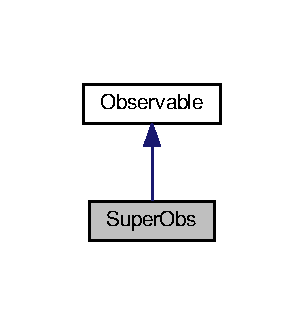
\includegraphics[width=146pt]{classSuperObs__inherit__graph}
\end{center}
\end{figure}


Collaboration diagram for Super\+Obs\+:\nopagebreak
\begin{figure}[H]
\begin{center}
\leavevmode
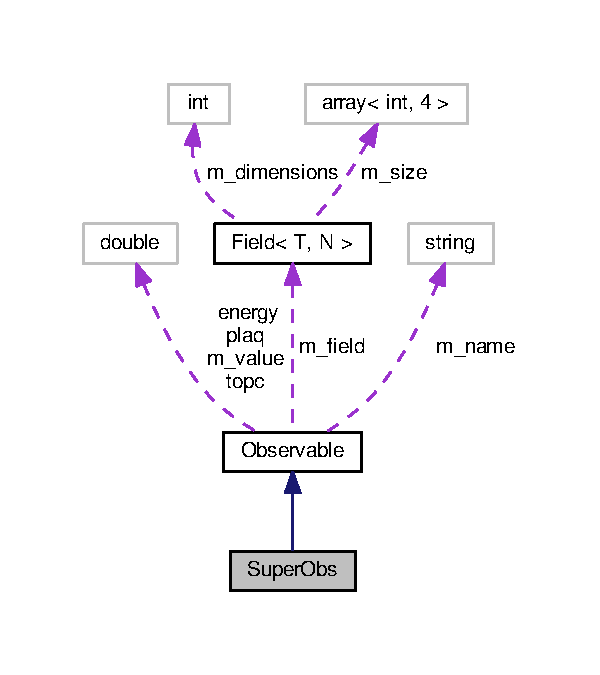
\includegraphics[width=288pt]{classSuperObs__coll__graph}
\end{center}
\end{figure}
\subsection*{Public Member Functions}
\begin{DoxyCompactItemize}
\item 
void {\bfseries init\+Observable} (\hyperlink{classField}{Gluon\+Field} $\ast$field)\hypertarget{classSuperObs_a292660868f04e6afc8c1300ec6fca5cc}{}\label{classSuperObs_a292660868f04e6afc8c1300ec6fca5cc}

\item 
void {\bfseries compute} ()\hypertarget{classSuperObs_a84e5e240fca5bdab31046fa87805456d}{}\label{classSuperObs_a84e5e240fca5bdab31046fa87805456d}

\end{DoxyCompactItemize}
\subsection*{Additional Inherited Members}


The documentation for this class was generated from the following files\+:\begin{DoxyCompactItemize}
\item 
/home/giovanni/\+Desktop/\+Lattice\+Yang\+Mills/include/\+Observables/superobs.\+h\item 
/home/giovanni/\+Desktop/\+Lattice\+Yang\+Mills/src/\+Observables/superobs.\+cpp\end{DoxyCompactItemize}

\hypertarget{classTopologicalCharge}{}\section{Topological\+Charge Class Reference}
\label{classTopologicalCharge}\index{Topological\+Charge@{Topological\+Charge}}


Implementation of the Topological Charge operator class.  




{\ttfamily \#include $<$topologicalcharge.\+h$>$}



Inheritance diagram for Topological\+Charge\+:\nopagebreak
\begin{figure}[H]
\begin{center}
\leavevmode
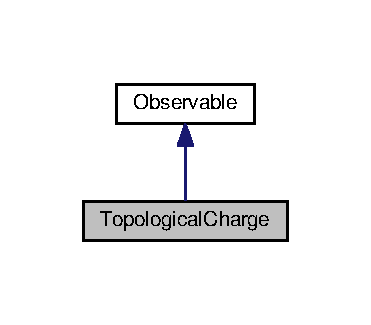
\includegraphics[width=178pt]{d6/de5/classTopologicalCharge__inherit__graph}
\end{center}
\end{figure}


Collaboration diagram for Topological\+Charge\+:\nopagebreak
\begin{figure}[H]
\begin{center}
\leavevmode
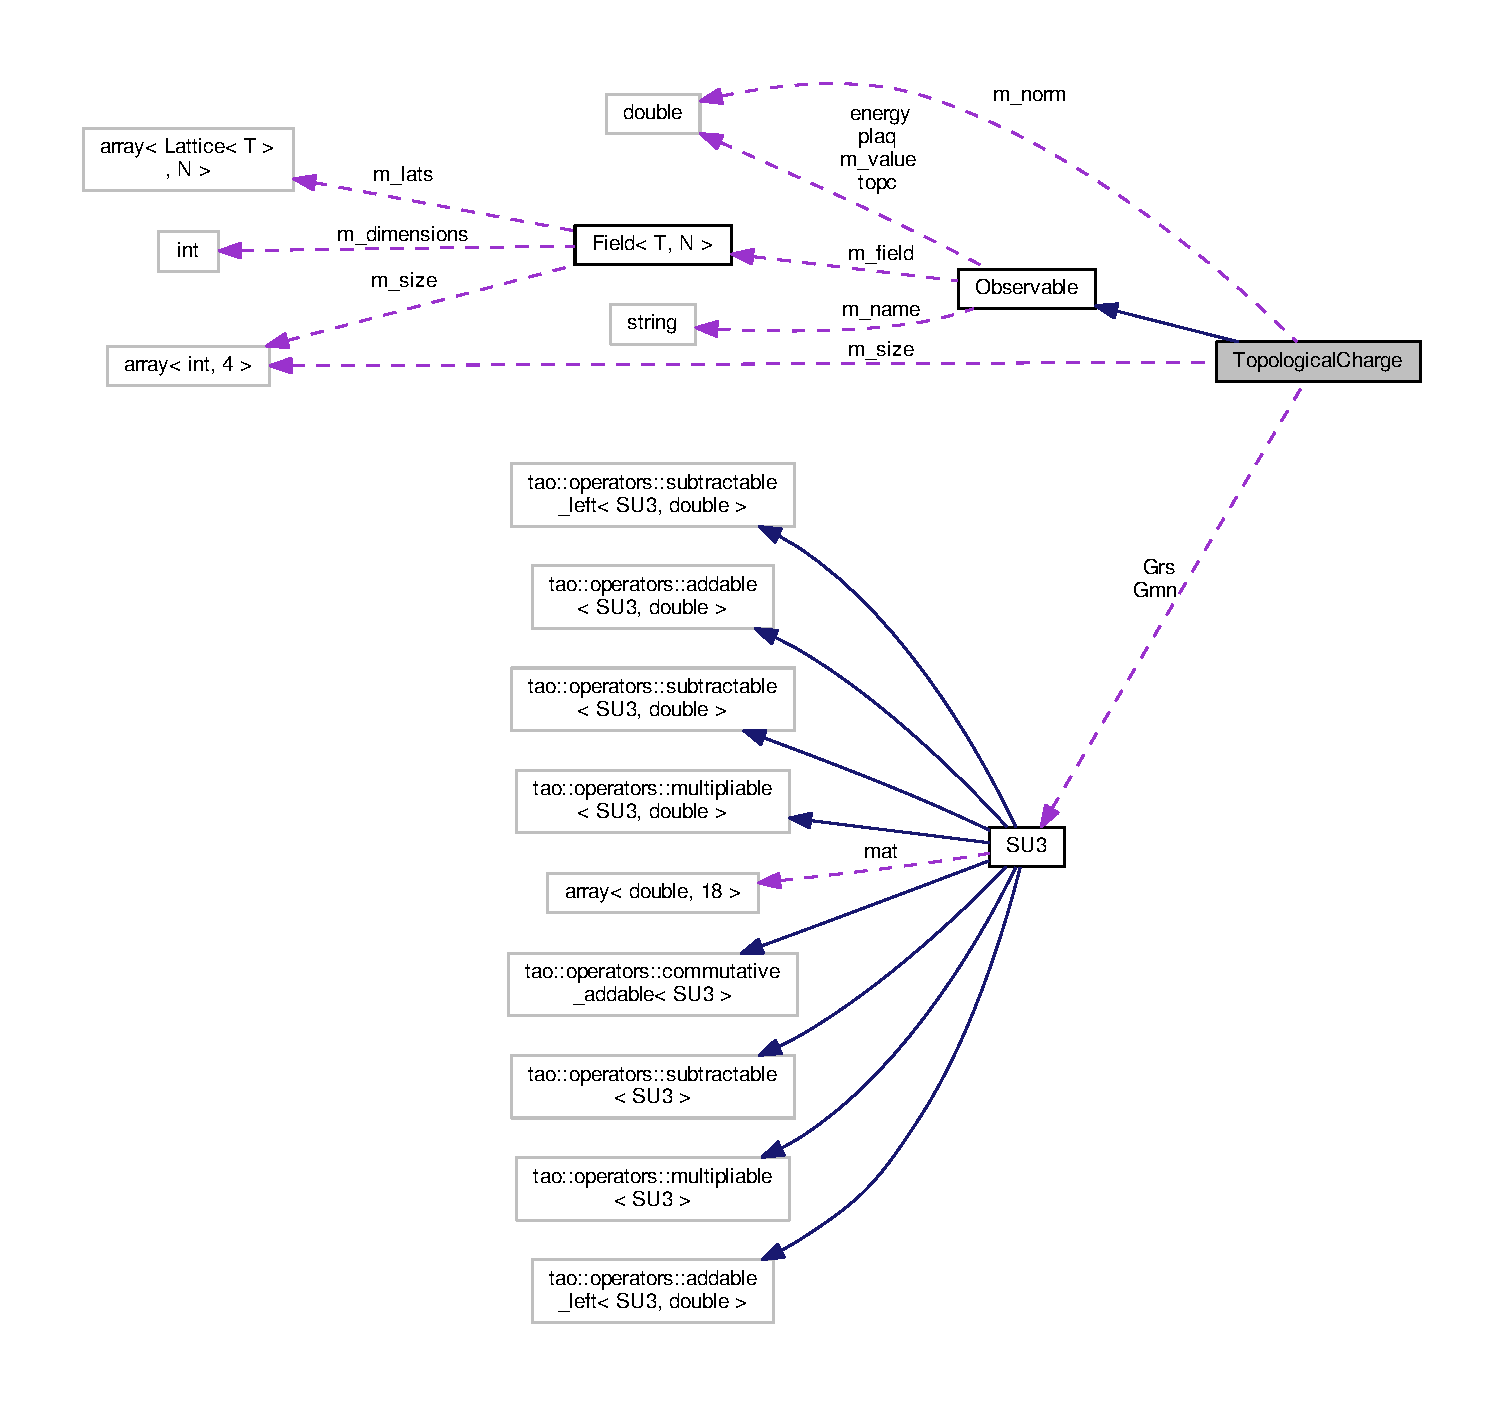
\includegraphics[width=350pt]{d1/dab/classTopologicalCharge__coll__graph}
\end{center}
\end{figure}
\subsection*{Public Member Functions}
\begin{DoxyCompactItemize}
\item 
void {\bfseries init\+Observable} (\hyperlink{classLattice}{Lattice} $\ast$lattice)\hypertarget{classTopologicalCharge_a3738265d7e456997ba0ff57bcba55188}{}\label{classTopologicalCharge_a3738265d7e456997ba0ff57bcba55188}

\item 
void {\bfseries compute} ()\hypertarget{classTopologicalCharge_a67b19b74c8c4f981d37490623ca774f2}{}\label{classTopologicalCharge_a67b19b74c8c4f981d37490623ca774f2}

\end{DoxyCompactItemize}
\subsection*{Private Attributes}
\begin{DoxyCompactItemize}
\item 
std\+::array$<$ int, 4 $>$ {\bfseries m\+\_\+size}\hypertarget{classTopologicalCharge_a7c710f7c182d1255533438fb343cf8ee}{}\label{classTopologicalCharge_a7c710f7c182d1255533438fb343cf8ee}

\item 
double {\bfseries m\+\_\+norm}\hypertarget{classTopologicalCharge_a35210a65883371d53d0eecbf90ef3ffd}{}\label{classTopologicalCharge_a35210a65883371d53d0eecbf90ef3ffd}

\item 
\hyperlink{structSU3}{S\+U3} {\bfseries Gmn}\hypertarget{classTopologicalCharge_a428ef097640a91fe39c3b2936cd64ad0}{}\label{classTopologicalCharge_a428ef097640a91fe39c3b2936cd64ad0}

\item 
\hyperlink{structSU3}{S\+U3} {\bfseries Grs}\hypertarget{classTopologicalCharge_a65cd1f2ba971ec5e92b60188b94b1a33}{}\label{classTopologicalCharge_a65cd1f2ba971ec5e92b60188b94b1a33}

\end{DoxyCompactItemize}
\subsection*{Additional Inherited Members}


\subsection{Detailed Description}
Implementation of the Topological Charge operator class. 

\begin{DoxyAuthor}{Author}
Giovanni Pederiva 
\end{DoxyAuthor}
\begin{DoxyVersion}{Version}
0.\+1 
\end{DoxyVersion}
\begin{DoxyDate}{Date}
2017-\/2018 
\end{DoxyDate}
\begin{DoxyCopyright}{Copyright}
M\+IT License.
\end{DoxyCopyright}
Old implementation of the Topological Charge operator class using the clover definition of the \hyperlink{classField}{Field} Stength Tensor 

Definition at line 50 of file topologicalcharge.\+h.



The documentation for this class was generated from the following files\+:\begin{DoxyCompactItemize}
\item 
\hyperlink{topologicalcharge_8h}{topologicalcharge.\+h}\item 
topologicalcharge.\+cpp\end{DoxyCompactItemize}

\hypertarget{classWilsonFlow}{}\section{Wilson\+Flow Class Reference}
\label{classWilsonFlow}\index{Wilson\+Flow@{Wilson\+Flow}}


Inheritance diagram for Wilson\+Flow\+:\nopagebreak
\begin{figure}[H]
\begin{center}
\leavevmode
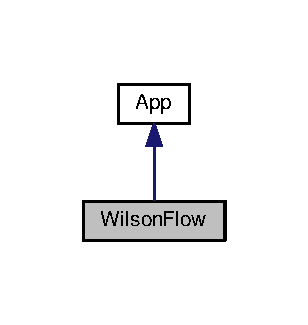
\includegraphics[width=148pt]{d3/d84/classWilsonFlow__inherit__graph}
\end{center}
\end{figure}


Collaboration diagram for Wilson\+Flow\+:
\nopagebreak
\begin{figure}[H]
\begin{center}
\leavevmode
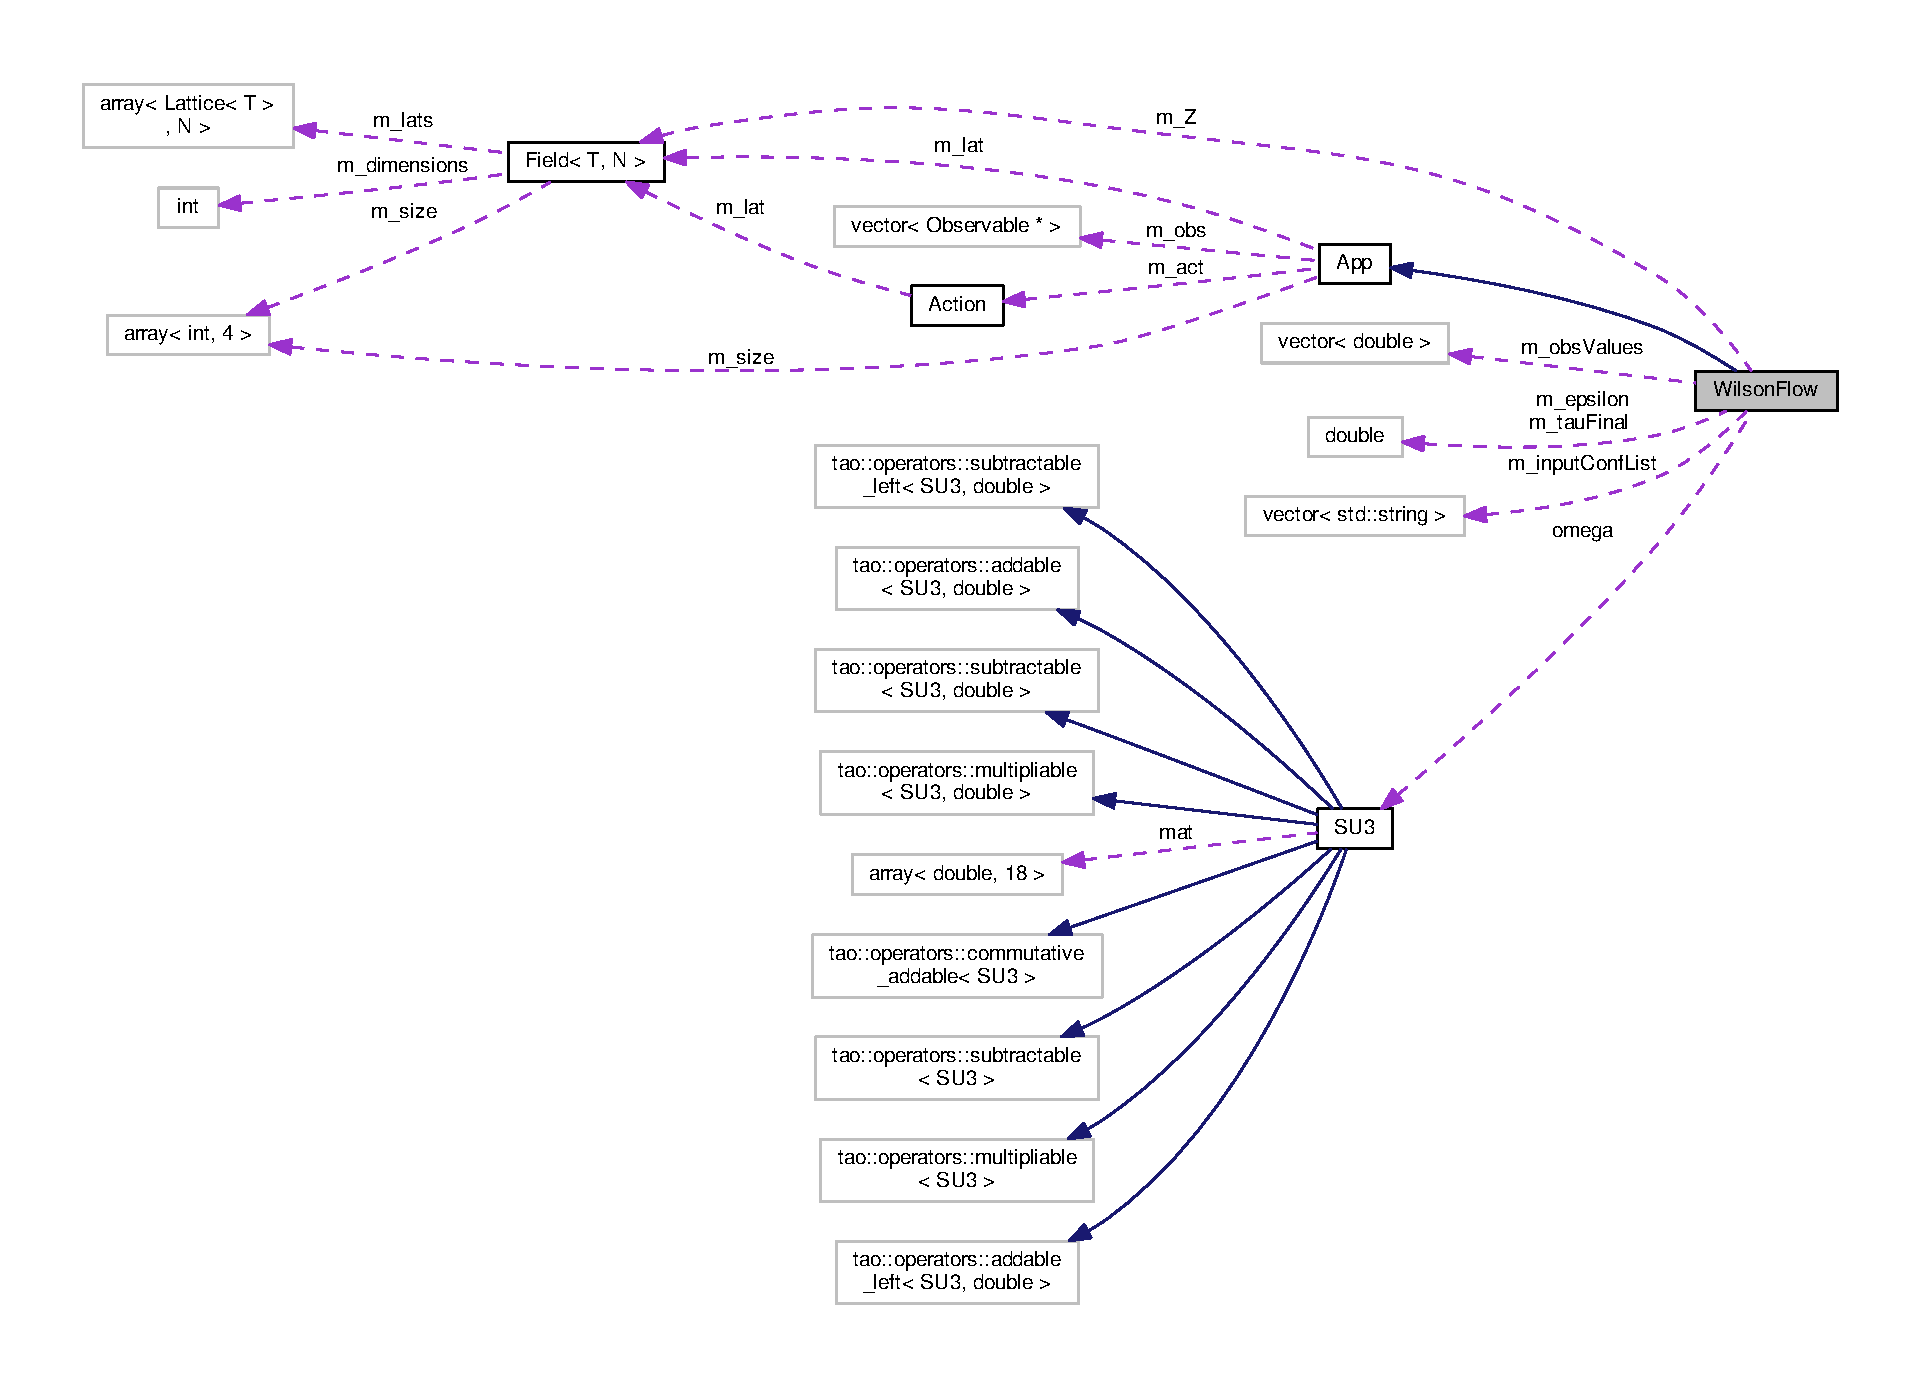
\includegraphics[width=350pt]{d6/da6/classWilsonFlow__coll__graph}
\end{center}
\end{figure}
\subsection*{Public Member Functions}
\begin{DoxyCompactItemize}
\item 
{\bfseries Wilson\+Flow} (double tau\+Final, double epsilon)\hypertarget{classWilsonFlow_a0ab55b82c101e093397192bbfa658609}{}\label{classWilsonFlow_a0ab55b82c101e093397192bbfa658609}

\item 
void {\bfseries flow\+Configurations} ()\hypertarget{classWilsonFlow_aff7b61f80cd9d4aa6d19e7281b2016d1}{}\label{classWilsonFlow_aff7b61f80cd9d4aa6d19e7281b2016d1}

\item 
void {\bfseries set\+Action} (\hyperlink{classAction}{Action} $\ast$action)\hypertarget{classWilsonFlow_a6b9ddd40b8165511df3fced3405ed593}{}\label{classWilsonFlow_a6b9ddd40b8165511df3fced3405ed593}

\item 
void {\bfseries add\+Observable} (\hyperlink{classObservable}{Observable} $\ast$observable)\hypertarget{classWilsonFlow_a0298e3a3e1b963c127abca860b61a4a4}{}\label{classWilsonFlow_a0298e3a3e1b963c127abca860b61a4a4}

\item 
std\+::array$<$ int, 4 $>$ \& {\bfseries get\+Size} ()\hypertarget{classWilsonFlow_ad00fa2dc5a90ae26bef6cd99ec90edc0}{}\label{classWilsonFlow_ad00fa2dc5a90ae26bef6cd99ec90edc0}

\item 
std\+::vector$<$ double $>$ \& {\bfseries get\+Obs\+Values} ()\hypertarget{classWilsonFlow_adcdb166df76bbc40c0076f326a431314}{}\label{classWilsonFlow_adcdb166df76bbc40c0076f326a431314}

\item 
std\+::vector$<$ \hyperlink{classObservable}{Observable} $\ast$ $>$ \& {\bfseries get\+Obs} ()\hypertarget{classWilsonFlow_a7105cd0a7a50a6775aadf9f717ff3478}{}\label{classWilsonFlow_a7105cd0a7a50a6775aadf9f717ff3478}

\item 
void {\bfseries create\+Lattice} (std\+::array$<$ int, 4 $>$ lattice\+Size)\hypertarget{classWilsonFlow_a1ae84f31a7b54b423bbe1d76001468d1}{}\label{classWilsonFlow_a1ae84f31a7b54b423bbe1d76001468d1}

\item 
void {\bfseries execute} ()\hypertarget{classWilsonFlow_a300944faffcb90c69ba9e2b62fd31561}{}\label{classWilsonFlow_a300944faffcb90c69ba9e2b62fd31561}

\item 
void {\bfseries initialize} ()\hypertarget{classWilsonFlow_afc84f29eab27e12f9ff51417dd6cf984}{}\label{classWilsonFlow_afc84f29eab27e12f9ff51417dd6cf984}

\end{DoxyCompactItemize}
\subsection*{Private Member Functions}
\begin{DoxyCompactItemize}
\item 
void {\bfseries compute\+Observables} ()\hypertarget{classWilsonFlow_aa9e371b2e2b8b1a24b372030dea6859b}{}\label{classWilsonFlow_aa9e371b2e2b8b1a24b372030dea6859b}

\item 
void {\bfseries flow\+Step} (double epsilon)\hypertarget{classWilsonFlow_a0ae15ce6735575690b3617f79e6cb20f}{}\label{classWilsonFlow_a0ae15ce6735575690b3617f79e6cb20f}

\item 
void {\bfseries apply\+Wilson\+Flow} (int conf\+Num, double epsilon)\hypertarget{classWilsonFlow_a72e7dc884133185d7f5410d212dfe4d5}{}\label{classWilsonFlow_a72e7dc884133185d7f5410d212dfe4d5}

\end{DoxyCompactItemize}
\subsection*{Private Attributes}
\begin{DoxyCompactItemize}
\item 
\hyperlink{classField}{Gluon\+Field} $\ast$ {\bfseries m\+\_\+Z} = nullptr\hypertarget{classWilsonFlow_ad084fea2d78728ce9f3891c8c6cb475f}{}\label{classWilsonFlow_ad084fea2d78728ce9f3891c8c6cb475f}

\item 
std\+::vector$<$ double $>$ {\bfseries m\+\_\+obs\+Values}\hypertarget{classWilsonFlow_a4c77c1ecf832e6da041ec430cbfec401}{}\label{classWilsonFlow_a4c77c1ecf832e6da041ec430cbfec401}

\item 
std\+::vector$<$ std\+::string $>$ {\bfseries m\+\_\+input\+Conf\+List}\hypertarget{classWilsonFlow_a7dadedd9bdec4647e512248d3627d08c}{}\label{classWilsonFlow_a7dadedd9bdec4647e512248d3627d08c}

\item 
\hyperlink{structSU3}{S\+U3} {\bfseries omega}\hypertarget{classWilsonFlow_a991660c79ba24a305baa7bdf6ea146d8}{}\label{classWilsonFlow_a991660c79ba24a305baa7bdf6ea146d8}

\item 
double {\bfseries m\+\_\+epsilon}\hypertarget{classWilsonFlow_a83a352e3cb1cc2a39d48dd96d8e7e581}{}\label{classWilsonFlow_a83a352e3cb1cc2a39d48dd96d8e7e581}

\item 
double {\bfseries m\+\_\+tau\+Final}\hypertarget{classWilsonFlow_abe5e34f28b9bd915a0a39d44df1d8d4a}{}\label{classWilsonFlow_abe5e34f28b9bd915a0a39d44df1d8d4a}

\end{DoxyCompactItemize}
\subsection*{Additional Inherited Members}


The documentation for this class was generated from the following files\+:\begin{DoxyCompactItemize}
\item 
wilsonflow.\+h\item 
wilsonflow.\+cpp\end{DoxyCompactItemize}

\chapter{File Documentation}
\hypertarget{action_8cpp}{}\section{action.\+cpp File Reference}
\label{action_8cpp}\index{action.\+cpp@{action.\+cpp}}


Details of the \hyperlink{classAction}{Action} prototype class.  


{\ttfamily \#include \char`\"{}Actions/action.\+h\char`\"{}}\\*
{\ttfamily \#include \char`\"{}Math/lattice.\+h\char`\"{}}\\*
Include dependency graph for action.\+cpp\+:\nopagebreak
\begin{figure}[H]
\begin{center}
\leavevmode
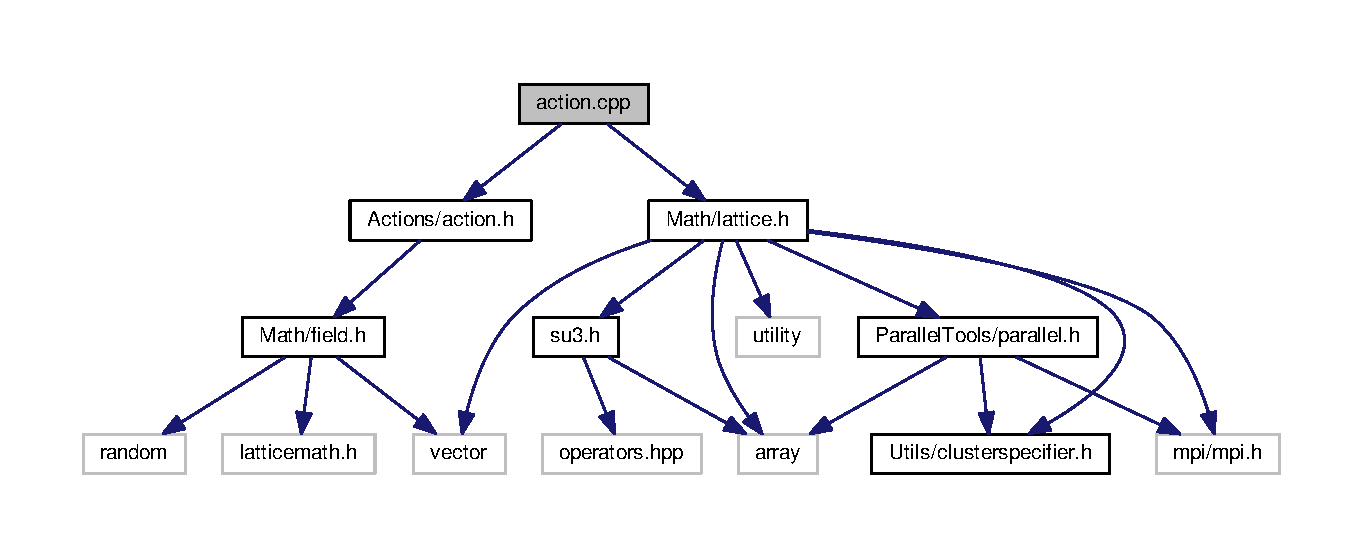
\includegraphics[width=350pt]{d0/d56/action_8cpp__incl}
\end{center}
\end{figure}


\subsection{Detailed Description}
Details of the \hyperlink{classAction}{Action} prototype class. 

\begin{DoxyAuthor}{Author}
Giovanni Pederiva 
\end{DoxyAuthor}
\begin{DoxyVersion}{Version}
1.\+0 
\end{DoxyVersion}
\begin{DoxyDate}{Date}
2017-\/2018 
\end{DoxyDate}
\begin{DoxyCopyright}{Copyright}
M\+IT License. 
\end{DoxyCopyright}

\hypertarget{action_8h}{}\section{action.\+h File Reference}
\label{action_8h}\index{action.\+h@{action.\+h}}


Contains the definition of the \hyperlink{classAction}{Action} prototype.  


{\ttfamily \#include \char`\"{}Math/field.\+h\char`\"{}}\\*
Include dependency graph for action.\+h\+:\nopagebreak
\begin{figure}[H]
\begin{center}
\leavevmode
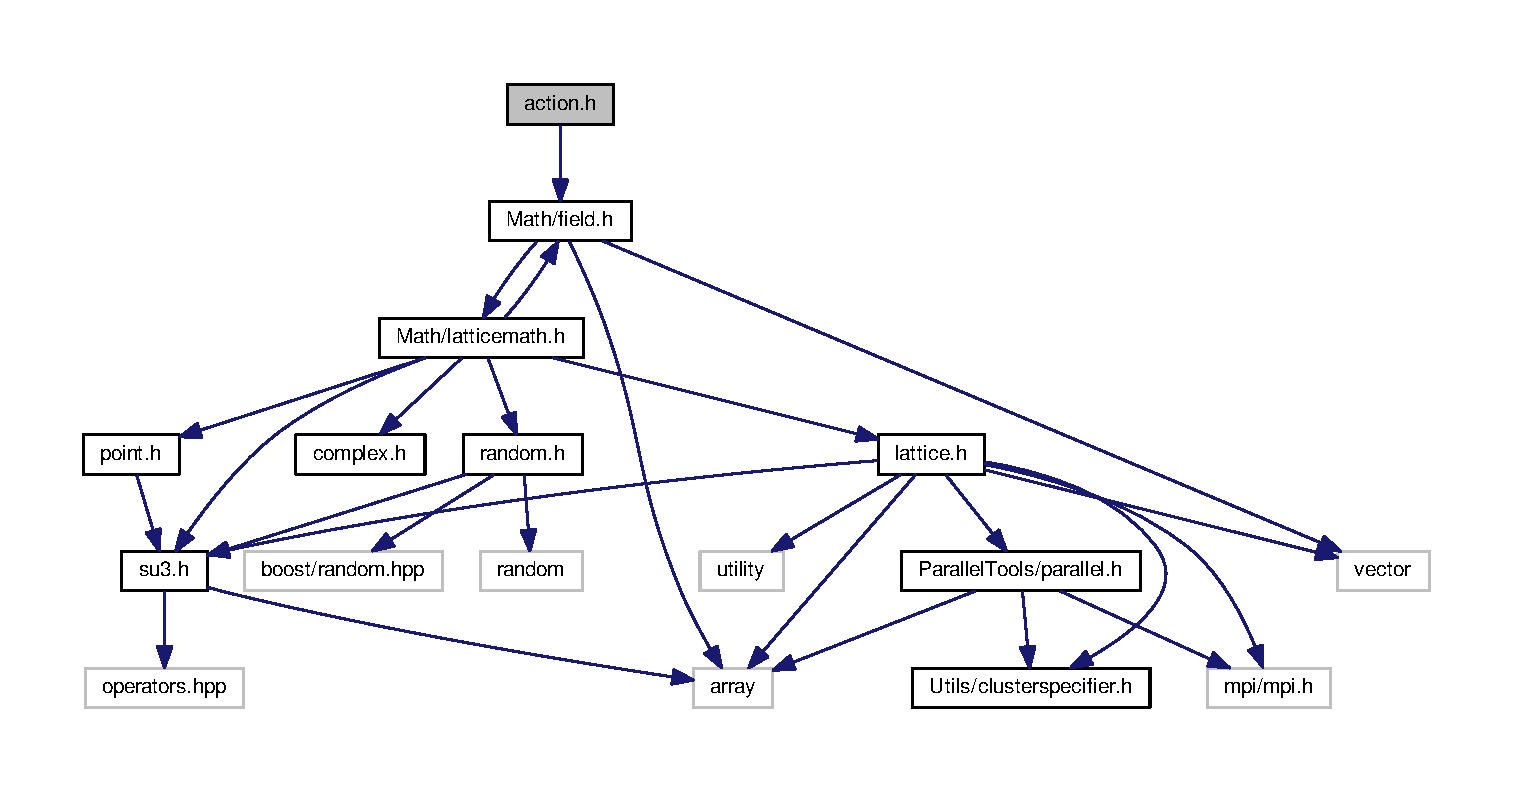
\includegraphics[width=350pt]{d0/d0a/action_8h__incl}
\end{center}
\end{figure}
This graph shows which files directly or indirectly include this file\+:\nopagebreak
\begin{figure}[H]
\begin{center}
\leavevmode
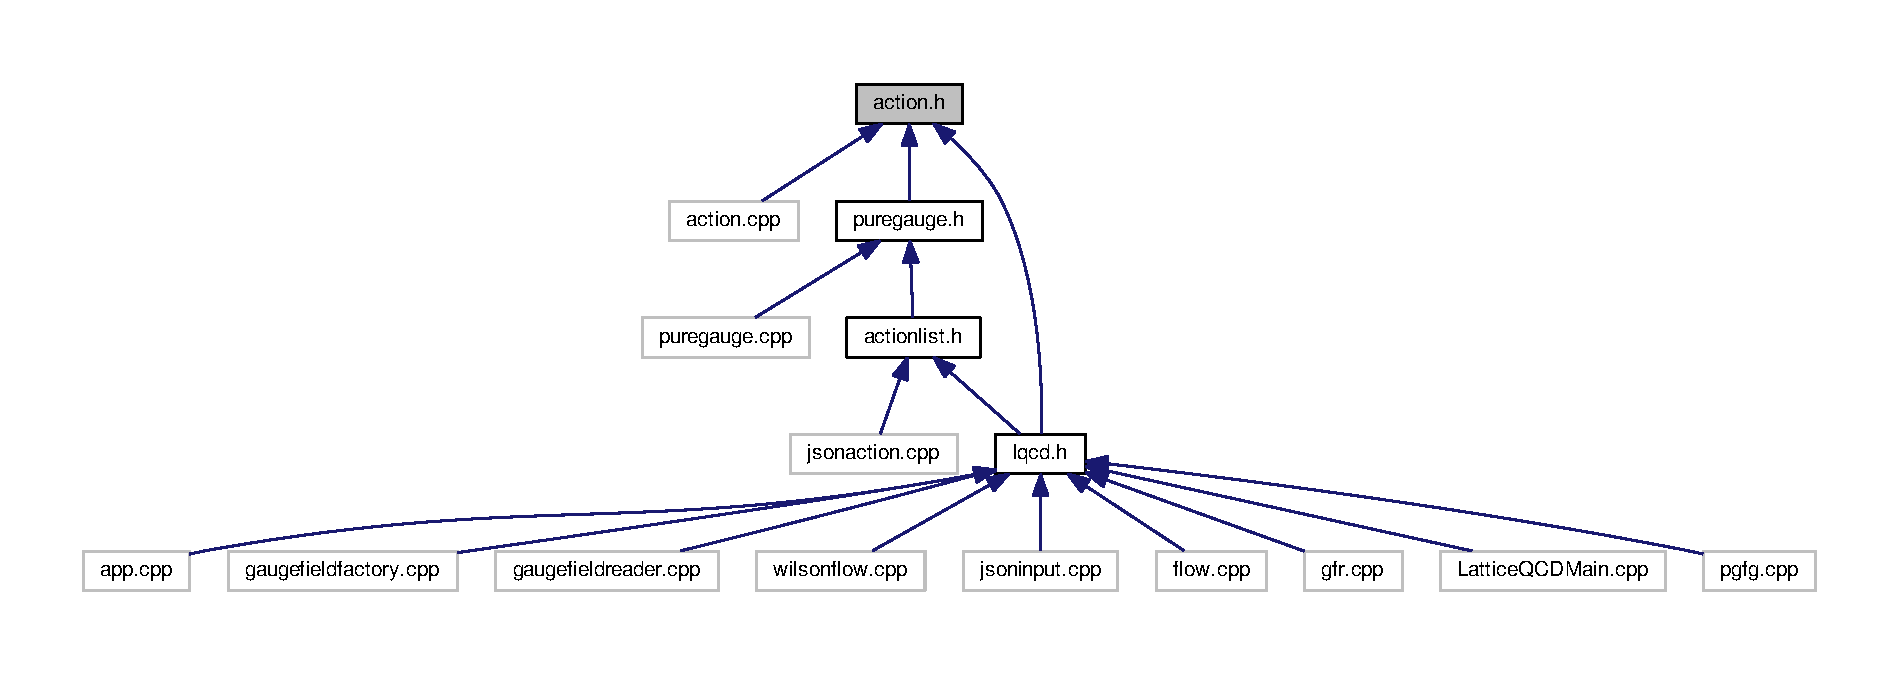
\includegraphics[width=350pt]{d8/dfe/action_8h__dep__incl}
\end{center}
\end{figure}
\subsection*{Classes}
\begin{DoxyCompactItemize}
\item 
class \hyperlink{classLattice}{Lattice$<$ T $>$}
\begin{DoxyCompactList}\small\item\em Template class to store an array with 4 dimensional indices of a given datatype. Includes functionalities for parallel shifts. \end{DoxyCompactList}\item 
class \hyperlink{classAction}{Action}
\begin{DoxyCompactList}\small\item\em Prototype for the \hyperlink{classAction}{Action} class group. \end{DoxyCompactList}\end{DoxyCompactItemize}


\subsection{Detailed Description}
Contains the definition of the \hyperlink{classAction}{Action} prototype. 

\begin{DoxyAuthor}{Author}
Giovanni Pederiva 
\end{DoxyAuthor}
\begin{DoxyVersion}{Version}
1.\+0 
\end{DoxyVersion}
\begin{DoxyDate}{Date}
2017-\/2018 
\end{DoxyDate}
\begin{DoxyCopyright}{Copyright}
M\+IT License. 
\end{DoxyCopyright}

\hypertarget{actionlist_8h}{}\section{actionlist.\+h File Reference}
\label{actionlist_8h}\index{actionlist.\+h@{actionlist.\+h}}


Main include file for \hyperlink{classAction}{Action} derived classes.  


{\ttfamily \#include \char`\"{}Actions/puregauge.\+h\char`\"{}}\\*
Include dependency graph for actionlist.\+h\+:\nopagebreak
\begin{figure}[H]
\begin{center}
\leavevmode
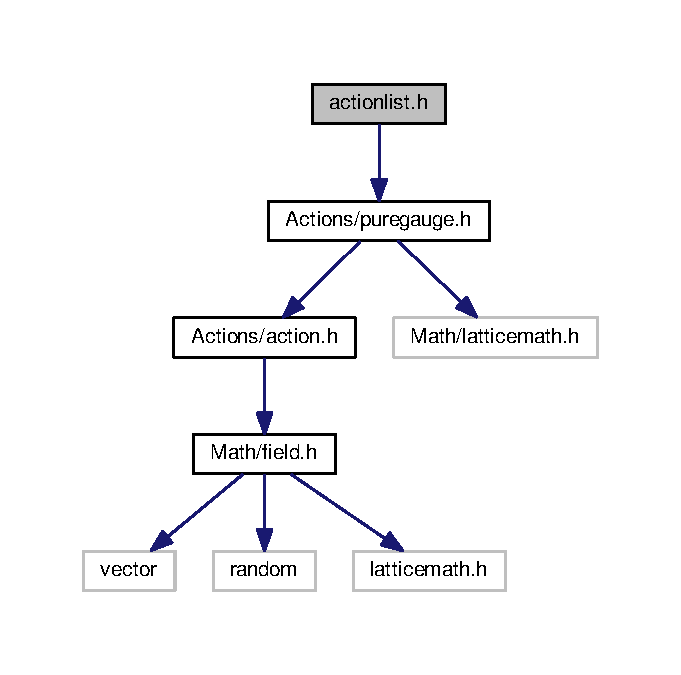
\includegraphics[width=327pt]{d4/d0f/actionlist_8h__incl}
\end{center}
\end{figure}
This graph shows which files directly or indirectly include this file\+:\nopagebreak
\begin{figure}[H]
\begin{center}
\leavevmode
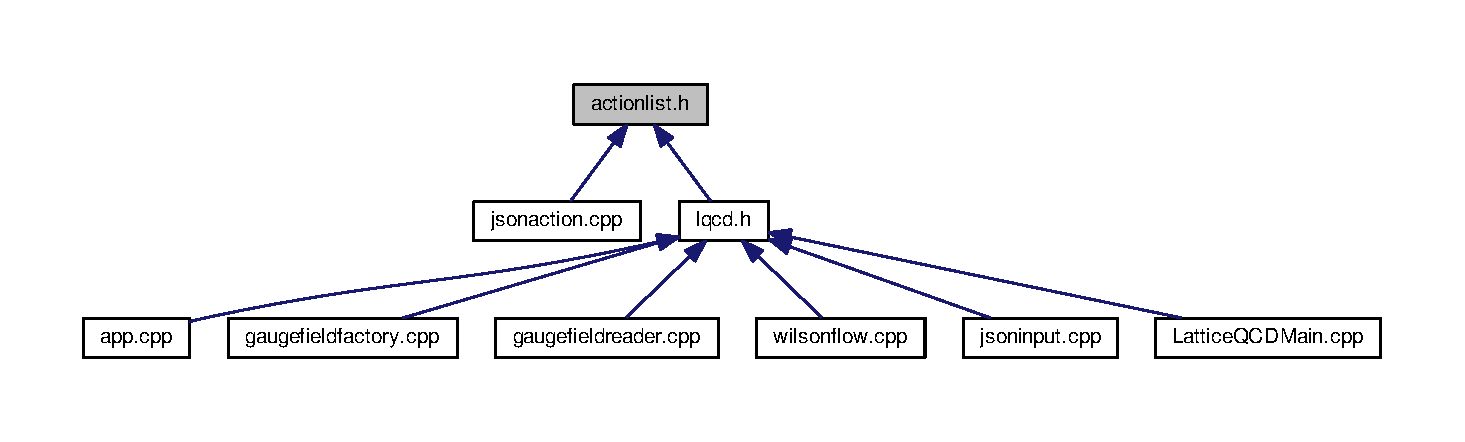
\includegraphics[width=350pt]{d7/dee/actionlist_8h__dep__incl}
\end{center}
\end{figure}


\subsection{Detailed Description}
Main include file for \hyperlink{classAction}{Action} derived classes. 

\begin{DoxyAuthor}{Author}
Giovanni Pederiva 
\end{DoxyAuthor}
\begin{DoxyVersion}{Version}
1.\+0 
\end{DoxyVersion}
\begin{DoxyDate}{Date}
2017-\/2018 
\end{DoxyDate}
\begin{DoxyCopyright}{Copyright}
M\+IT License.
\end{DoxyCopyright}
This file provides a simple access to all of the classes that implement the \hyperlink{classAction}{Action} type 
\hypertarget{app_8cpp}{}\section{app.\+cpp File Reference}
\label{app_8cpp}\index{app.\+cpp@{app.\+cpp}}


Contains the implementation of the \hyperlink{classApp}{App} prototype class methods.  


{\ttfamily \#include \char`\"{}lqcd.\+h\char`\"{}}\\*
Include dependency graph for app.\+cpp\+:
% FIG 0


\subsection{Detailed Description}
Contains the implementation of the \hyperlink{classApp}{App} prototype class methods. 

\begin{DoxyAuthor}{Author}
Giovanni Pederiva 
\end{DoxyAuthor}
\begin{DoxyVersion}{Version}
1.\+0 
\end{DoxyVersion}
\begin{DoxyDate}{Date}
2017-\/2018 
\end{DoxyDate}
\begin{DoxyCopyright}{Copyright}
M\+IT License. 
\end{DoxyCopyright}

\hypertarget{app_8h}{}\section{app.\+h File Reference}
\label{app_8h}\index{app.\+h@{app.\+h}}


Contains the definition of the \hyperlink{classApp}{App} prototype.  


{\ttfamily \#include $<$array$>$}\\*
{\ttfamily \#include $<$vector$>$}\\*
{\ttfamily \#include \char`\"{}Math/field.\+h\char`\"{}}\\*
{\ttfamily \#include \char`\"{}Observables/observable.\+h\char`\"{}}\\*
Include dependency graph for app.\+h\+:
% FIG 0
This graph shows which files directly or indirectly include this file\+:
% FIG 1
\subsection*{Classes}
\begin{DoxyCompactItemize}
\item 
class \hyperlink{classLattice}{Lattice$<$ T $>$}
\begin{DoxyCompactList}\small\item\em Template class to store an array with 4 dimensional indices of a given datatype. Includes functionalities for parallel shifts. \end{DoxyCompactList}\item 
class \hyperlink{classApp}{App}
\begin{DoxyCompactList}\small\item\em Prototype for the \hyperlink{classApp}{App} class group. \end{DoxyCompactList}\end{DoxyCompactItemize}


\subsection{Detailed Description}
Contains the definition of the \hyperlink{classApp}{App} prototype. 

\begin{DoxyAuthor}{Author}
Giovanni Pederiva 
\end{DoxyAuthor}
\begin{DoxyVersion}{Version}
1.\+0 
\end{DoxyVersion}
\begin{DoxyDate}{Date}
2017-\/2018 
\end{DoxyDate}
\begin{DoxyCopyright}{Copyright}
M\+IT License. 
\end{DoxyCopyright}

\hypertarget{applist_8h}{}\section{applist.\+h File Reference}
\label{applist_8h}\index{applist.\+h@{applist.\+h}}


Main include file for \hyperlink{classApp}{App} derived classes.  


{\ttfamily \#include \char`\"{}app.\+h\char`\"{}}\\*
{\ttfamily \#include \char`\"{}gaugefieldfactory.\+h\char`\"{}}\\*
{\ttfamily \#include \char`\"{}gaugefieldreader.\+h\char`\"{}}\\*
{\ttfamily \#include \char`\"{}wilsonflow.\+h\char`\"{}}\\*
Include dependency graph for applist.\+h\+:
% FIG 0
This graph shows which files directly or indirectly include this file\+:
% FIG 1


\subsection{Detailed Description}
Main include file for \hyperlink{classApp}{App} derived classes. 

\begin{DoxyAuthor}{Author}
Giovanni Pederiva 
\end{DoxyAuthor}
\begin{DoxyVersion}{Version}
1.\+0 
\end{DoxyVersion}
\begin{DoxyDate}{Date}
2017-\/2018 
\end{DoxyDate}
\begin{DoxyCopyright}{Copyright}
M\+IT License.
\end{DoxyCopyright}
This file provides a simple access to all of the classes that implement the \hyperlink{classApp}{App} type 
\hypertarget{energydensity_8cpp}{}\section{energydensity.\+cpp File Reference}
\label{energydensity_8cpp}\index{energydensity.\+cpp@{energydensity.\+cpp}}


Details of the energy density observable class (old)  


{\ttfamily \#include \char`\"{}Observables/energydensity.\+h\char`\"{}}\\*
{\ttfamily \#include \char`\"{}Observables/observable.\+h\char`\"{}}\\*
{\ttfamily \#include \char`\"{}Math/su3.\+h\char`\"{}}\\*
{\ttfamily \#include \char`\"{}Math/lattice.\+h\char`\"{}}\\*
{\ttfamily \#include $<$cstdio$>$}\\*
{\ttfamily \#include $<$cmath$>$}\\*
Include dependency graph for energydensity.\+cpp\+:\nopagebreak
\begin{figure}[H]
\begin{center}
\leavevmode
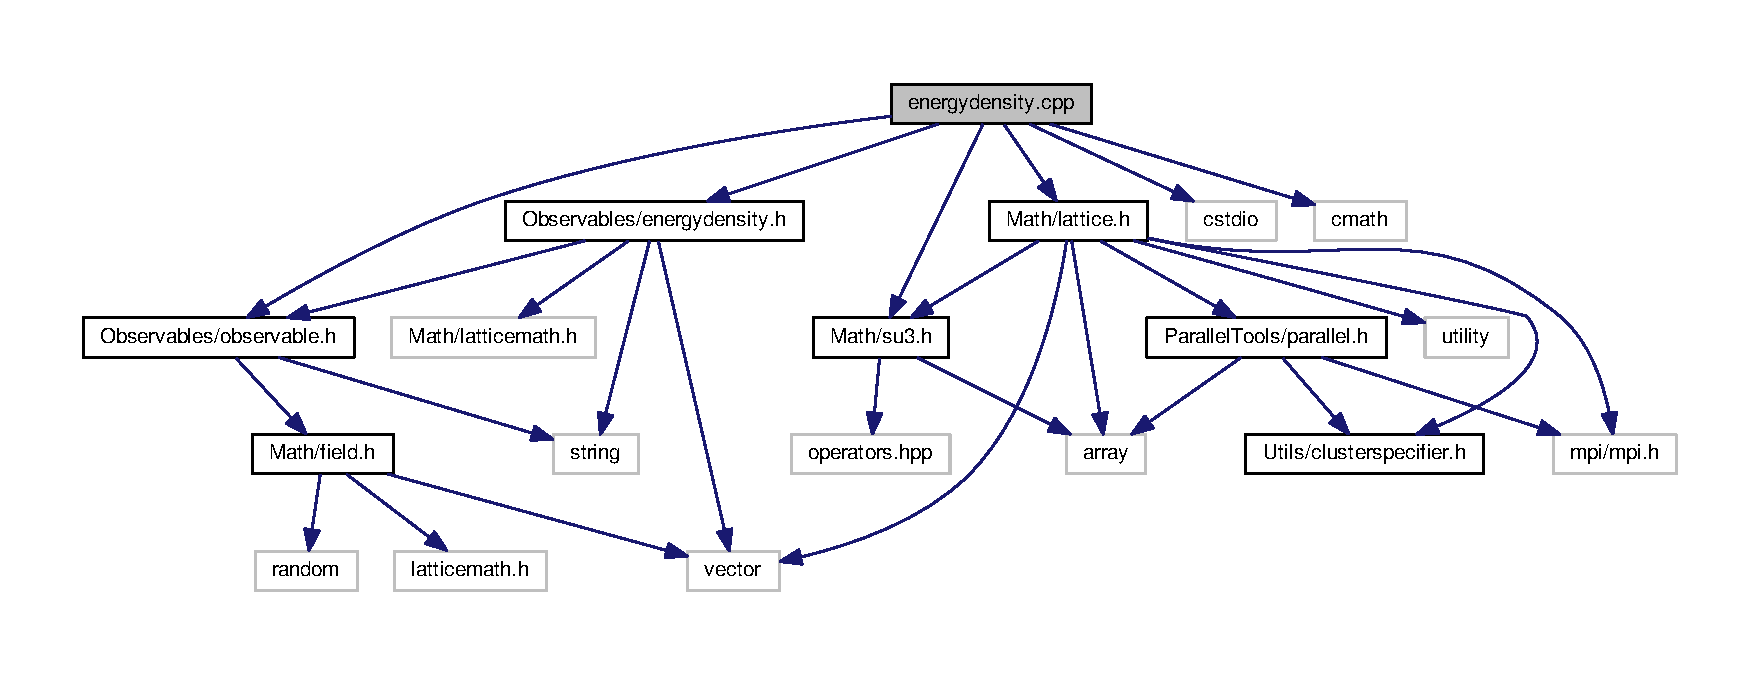
\includegraphics[width=350pt]{d3/d52/energydensity_8cpp__incl}
\end{center}
\end{figure}


\subsection{Detailed Description}
Details of the energy density observable class (old) 

\begin{DoxyAuthor}{Author}
Giovanni Pederiva 
\end{DoxyAuthor}
\begin{DoxyVersion}{Version}
0.\+1 
\end{DoxyVersion}
\begin{DoxyDate}{Date}
2017-\/2018 
\end{DoxyDate}
\begin{DoxyCopyright}{Copyright}
M\+IT License. 
\end{DoxyCopyright}

\hypertarget{energydensity_8h}{}\section{energydensity.\+h File Reference}
\label{energydensity_8h}\index{energydensity.\+h@{energydensity.\+h}}


Contains the definition of the \hyperlink{classEnergyDensity}{Energy\+Density} observable.  


{\ttfamily \#include $<$vector$>$}\\*
{\ttfamily \#include $<$string$>$}\\*
{\ttfamily \#include \char`\"{}Observables/observable.\+h\char`\"{}}\\*
{\ttfamily \#include \char`\"{}Math/latticemath.\+h\char`\"{}}\\*
Include dependency graph for energydensity.\+h\+:\nopagebreak
\begin{figure}[H]
\begin{center}
\leavevmode
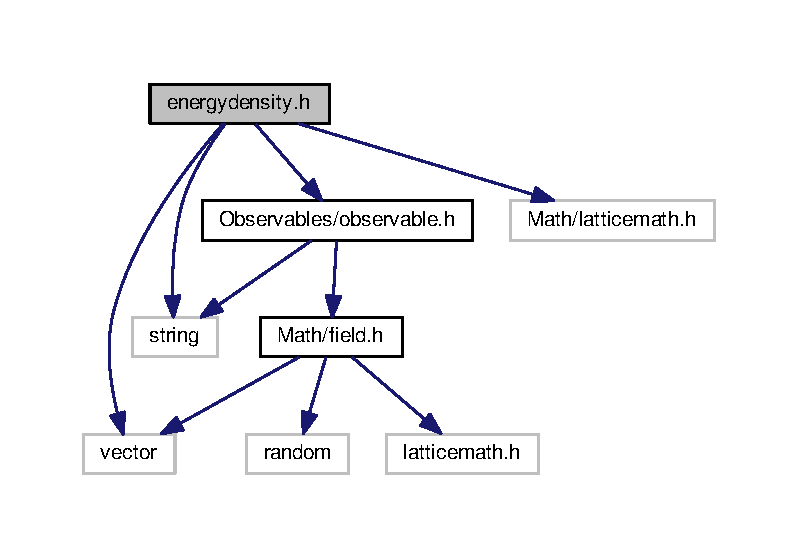
\includegraphics[width=350pt]{d2/daa/energydensity_8h__incl}
\end{center}
\end{figure}
This graph shows which files directly or indirectly include this file\+:\nopagebreak
\begin{figure}[H]
\begin{center}
\leavevmode
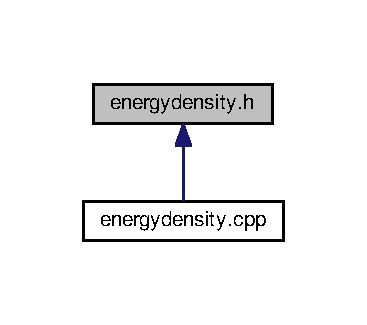
\includegraphics[width=176pt]{de/dd8/energydensity_8h__dep__incl}
\end{center}
\end{figure}
\subsection*{Classes}
\begin{DoxyCompactItemize}
\item 
class \hyperlink{classEnergyDensity}{Energy\+Density}
\begin{DoxyCompactList}\small\item\em Implementation of the Energy Density operator class. \end{DoxyCompactList}\end{DoxyCompactItemize}


\subsection{Detailed Description}
Contains the definition of the \hyperlink{classEnergyDensity}{Energy\+Density} observable. 

\begin{DoxyAuthor}{Author}
Giovanni Pederiva 
\end{DoxyAuthor}
\begin{DoxyVersion}{Version}
0.\+1 
\end{DoxyVersion}
\begin{DoxyDate}{Date}
2017-\/2018 
\end{DoxyDate}
\begin{DoxyCopyright}{Copyright}
M\+IT License. 
\end{DoxyCopyright}

\hypertarget{field_8h}{}\section{field.\+h File Reference}
\label{field_8h}\index{field.\+h@{field.\+h}}


Contains the definition of the \hyperlink{classField}{Field} class.  


{\ttfamily \#include $<$vector$>$}\\*
{\ttfamily \#include $<$random$>$}\\*
{\ttfamily \#include \char`\"{}latticemath.\+h\char`\"{}}\\*
Include dependency graph for field.\+h\+:\nopagebreak
\begin{figure}[H]
\begin{center}
\leavevmode
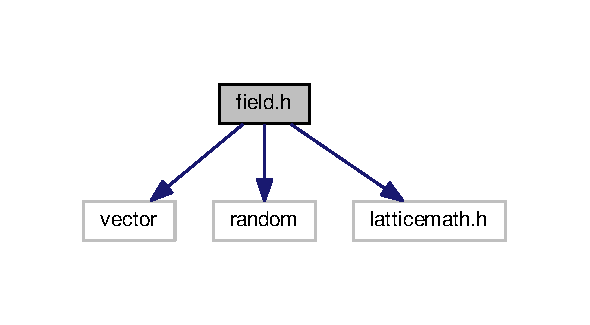
\includegraphics[width=283pt]{d7/d64/field_8h__incl}
\end{center}
\end{figure}
This graph shows which files directly or indirectly include this file\+:\nopagebreak
\begin{figure}[H]
\begin{center}
\leavevmode
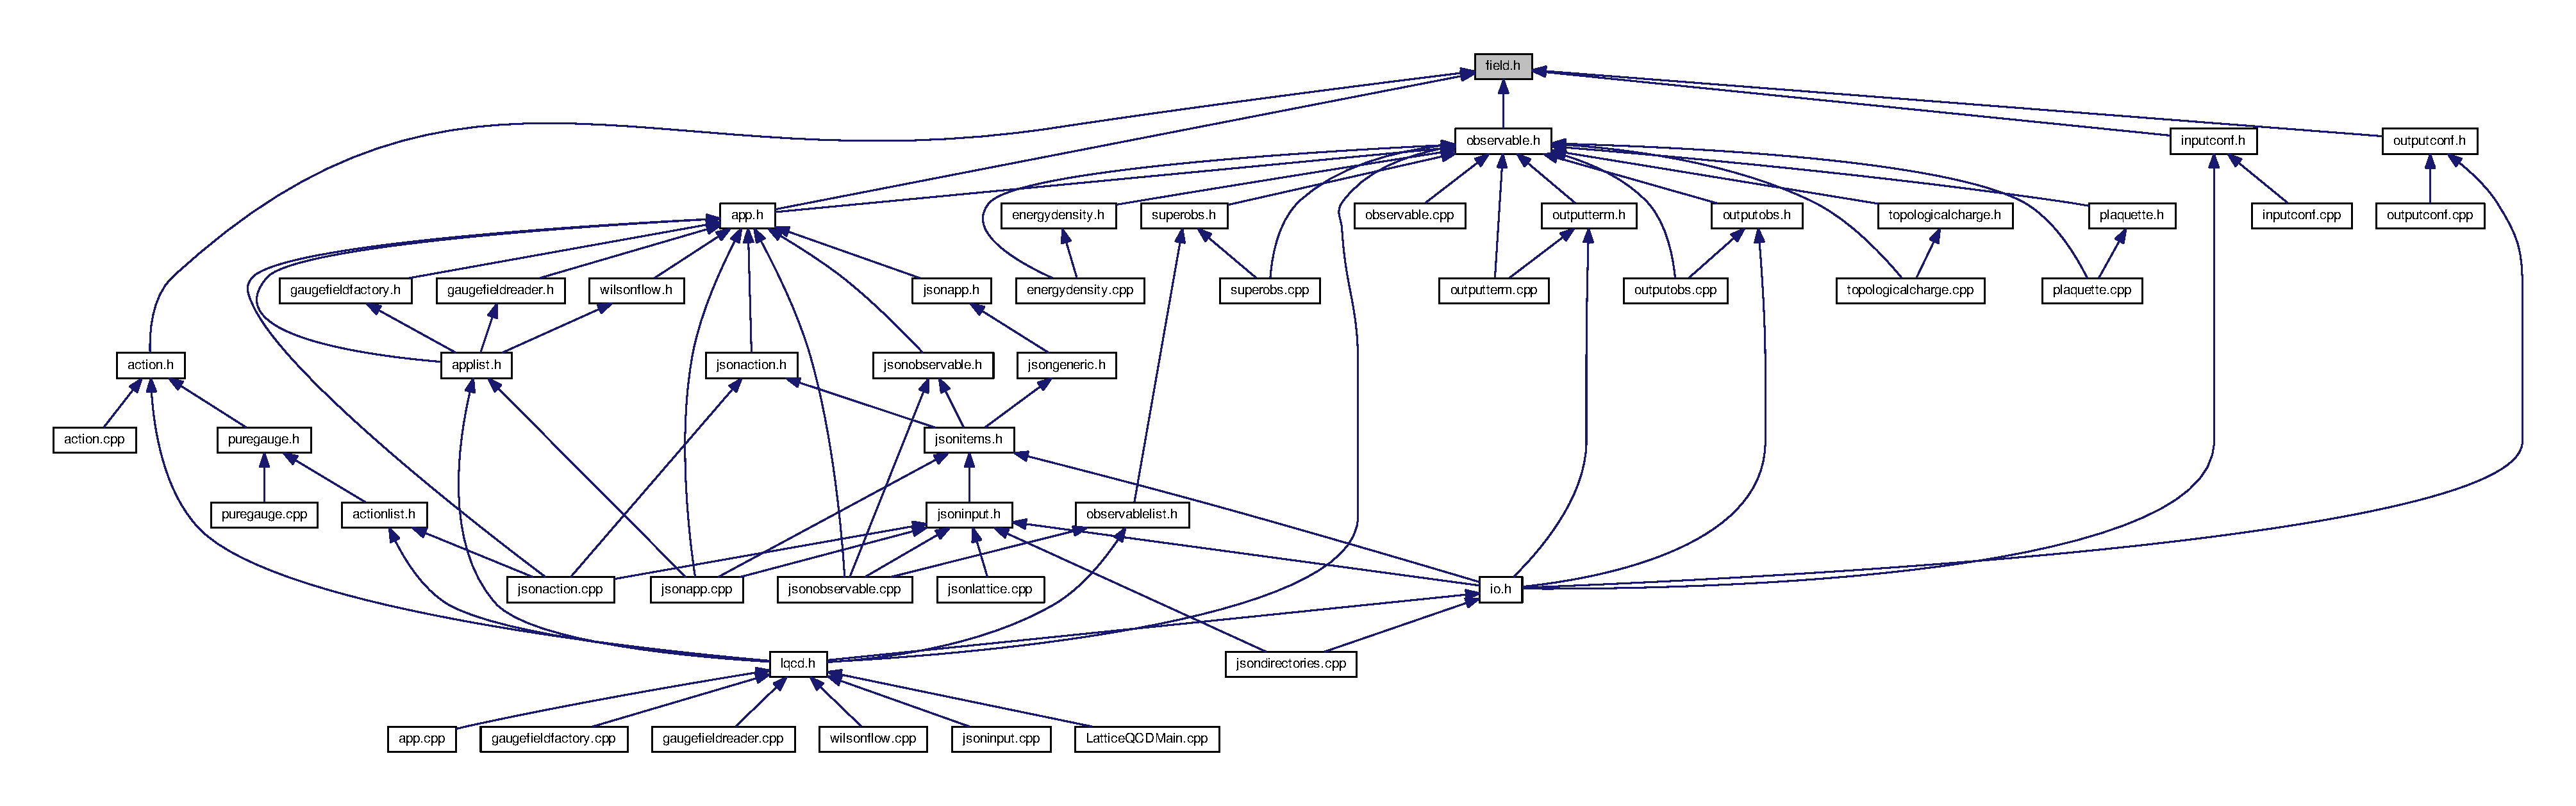
\includegraphics[width=350pt]{d6/d8f/field_8h__dep__incl}
\end{center}
\end{figure}
\subsection*{Classes}
\begin{DoxyCompactItemize}
\item 
class \hyperlink{classField}{Field$<$ T, N $>$}
\begin{DoxyCompactList}\small\item\em Class that represents the Q\+CD field as an array of 4 \hyperlink{structSU3}{S\+U3} lattices. \end{DoxyCompactList}\end{DoxyCompactItemize}
\subsection*{Typedefs}
\begin{DoxyCompactItemize}
\item 
typedef \hyperlink{classField}{Field}$<$ \hyperlink{structSU3}{S\+U3}, 4 $>$ \hyperlink{field_8h_afe80b127697eba6d6e7fbd8121c8d4ee}{Gluon\+Field}
\end{DoxyCompactItemize}


\subsection{Detailed Description}
Contains the definition of the \hyperlink{classField}{Field} class. 

\begin{DoxyAuthor}{Author}
Giovanni Pederiva 
\end{DoxyAuthor}
\begin{DoxyVersion}{Version}
1.\+0 
\end{DoxyVersion}
\begin{DoxyDate}{Date}
2017-\/2018 
\end{DoxyDate}
\begin{DoxyCopyright}{Copyright}
M\+IT License. 
\end{DoxyCopyright}


\subsection{Typedef Documentation}
\index{field.\+h@{field.\+h}!Gluon\+Field@{Gluon\+Field}}
\index{Gluon\+Field@{Gluon\+Field}!field.\+h@{field.\+h}}
\subsubsection[{\texorpdfstring{Gluon\+Field}{GluonField}}]{\setlength{\rightskip}{0pt plus 5cm}typedef {\bf Field}$<${\bf S\+U3},4$>$ {\bf Gluon\+Field}}\hypertarget{field_8h_afe80b127697eba6d6e7fbd8121c8d4ee}{}\label{field_8h_afe80b127697eba6d6e7fbd8121c8d4ee}
Convenience definition of the \hyperlink{structSU3}{S\+U3} case 4 dimensional case of a \hyperlink{classField}{Field} class, the Gluon\+Field 

Definition at line 76 of file field.\+h.


\hypertarget{gaugefieldfactory_8cpp}{}\section{gaugefieldfactory.\+cpp File Reference}
\label{gaugefieldfactory_8cpp}\index{gaugefieldfactory.\+cpp@{gaugefieldfactory.\+cpp}}


Contains the implementation of the \hyperlink{classGaugeFieldFactory}{Gauge\+Field\+Factory} class methods.  


{\ttfamily \#include $<$vector$>$}\\*
{\ttfamily \#include $<$cstdio$>$}\\*
{\ttfamily \#include $<$chrono$>$}\\*
{\ttfamily \#include \char`\"{}lqcd.\+h\char`\"{}}\\*
Include dependency graph for gaugefieldfactory.\+cpp\+:\nopagebreak
\begin{figure}[H]
\begin{center}
\leavevmode
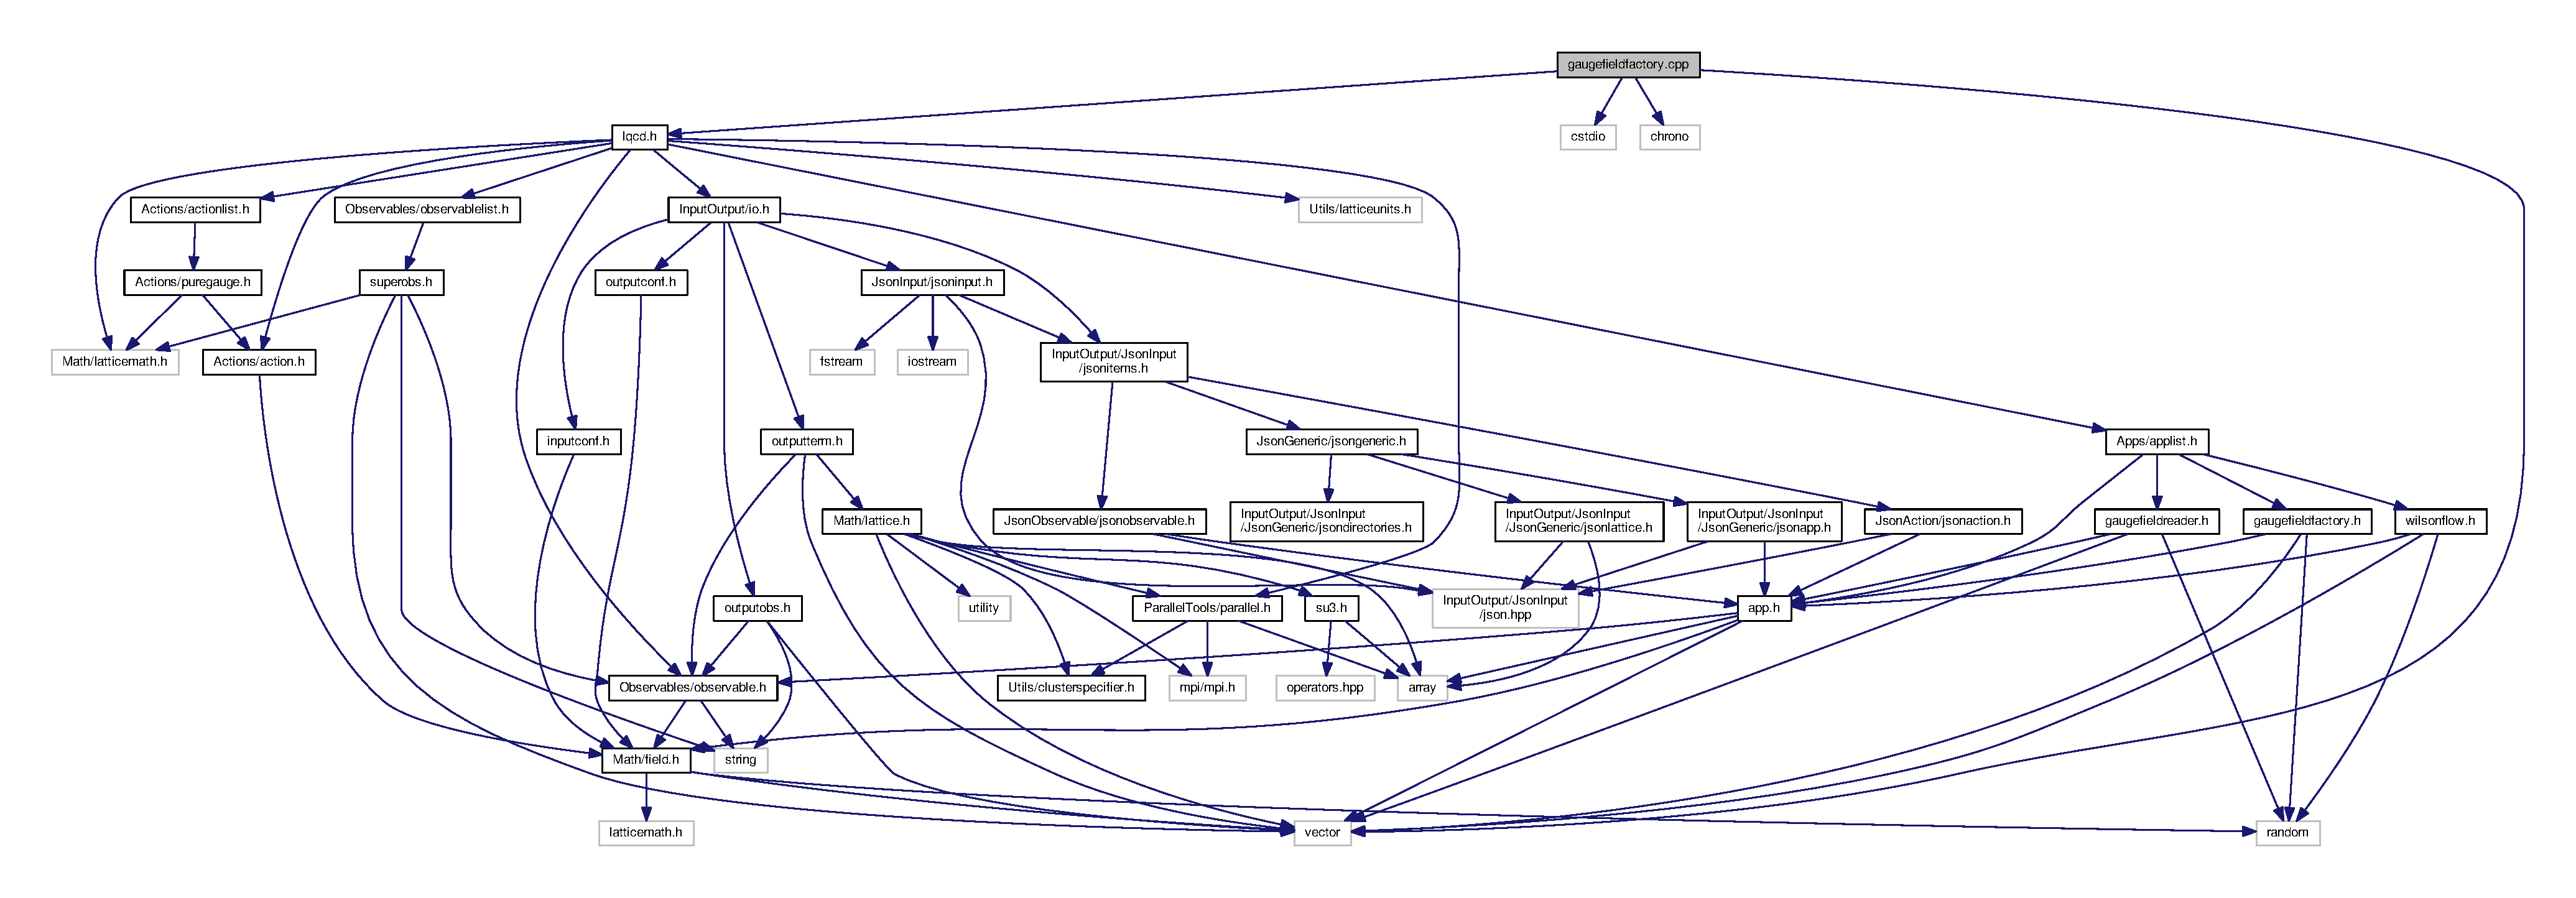
\includegraphics[width=350pt]{d0/dc1/gaugefieldfactory_8cpp__incl}
\end{center}
\end{figure}


\subsection{Detailed Description}
Contains the implementation of the \hyperlink{classGaugeFieldFactory}{Gauge\+Field\+Factory} class methods. 

\begin{DoxyAuthor}{Author}
Giovanni Pederiva 
\end{DoxyAuthor}
\begin{DoxyVersion}{Version}
1.\+0 
\end{DoxyVersion}
\begin{DoxyDate}{Date}
2017-\/2018 
\end{DoxyDate}
\begin{DoxyCopyright}{Copyright}
M\+IT License. 
\end{DoxyCopyright}

\hypertarget{gaugefieldfactory_8h}{}\section{gaugefieldfactory.\+h File Reference}
\label{gaugefieldfactory_8h}\index{gaugefieldfactory.\+h@{gaugefieldfactory.\+h}}


Contains the definition of the \hyperlink{classGaugeFieldFactory}{Gauge\+Field\+Factory} \hyperlink{classApp}{App} derived class.  


{\ttfamily \#include $<$vector$>$}\\*
{\ttfamily \#include $<$random$>$}\\*
{\ttfamily \#include \char`\"{}Apps/app.\+h\char`\"{}}\\*
Include dependency graph for gaugefieldfactory.\+h\+:\nopagebreak
\begin{figure}[H]
\begin{center}
\leavevmode
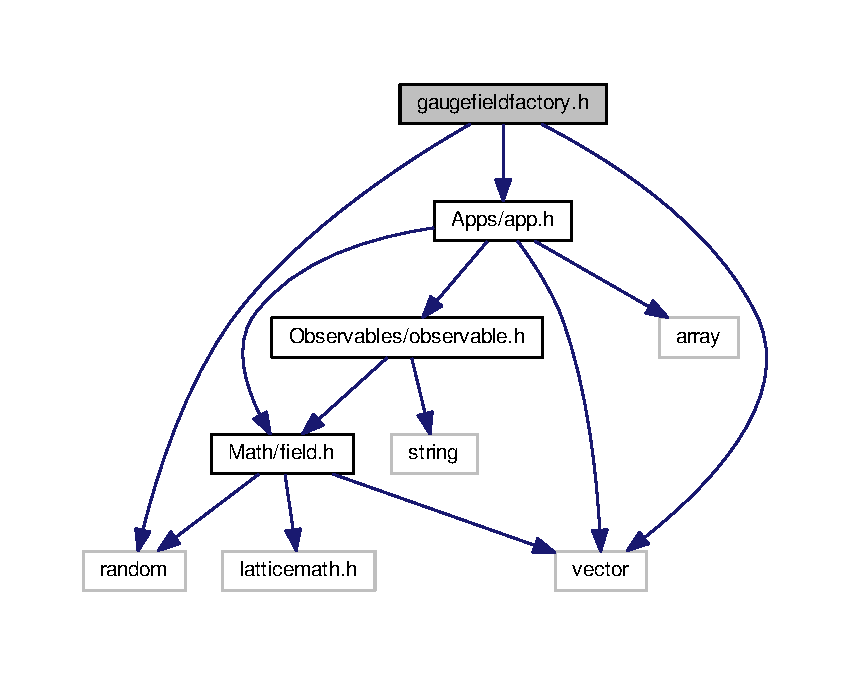
\includegraphics[width=350pt]{d6/d77/gaugefieldfactory_8h__incl}
\end{center}
\end{figure}
This graph shows which files directly or indirectly include this file\+:\nopagebreak
\begin{figure}[H]
\begin{center}
\leavevmode
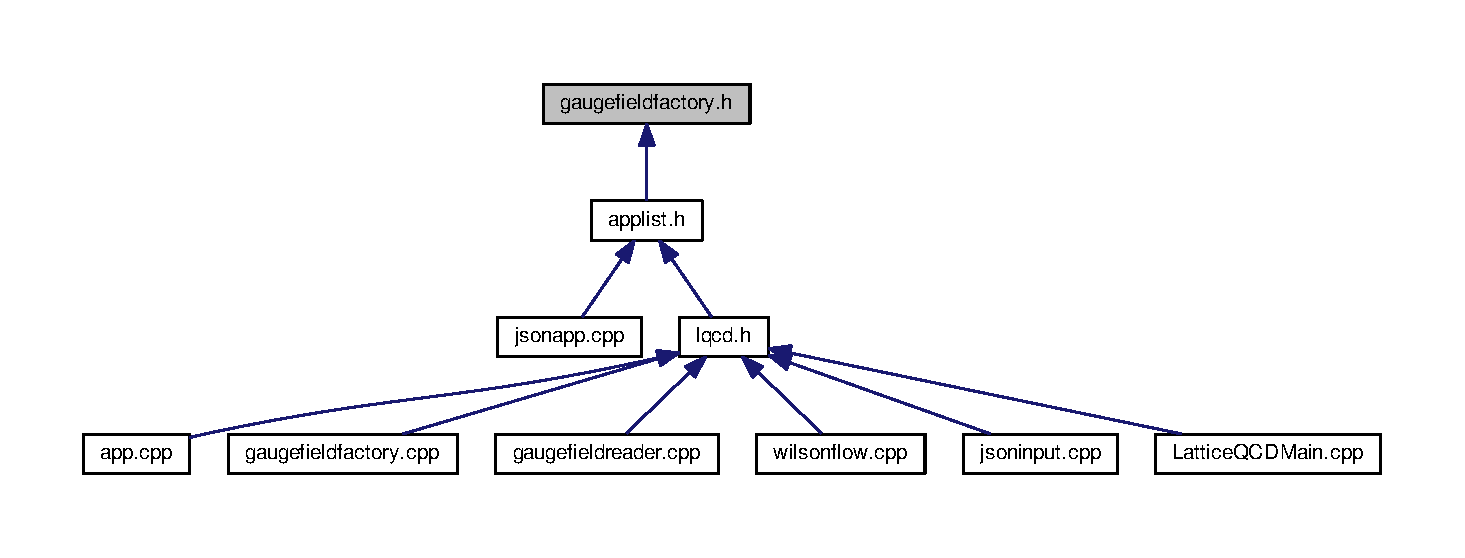
\includegraphics[width=350pt]{df/dc5/gaugefieldfactory_8h__dep__incl}
\end{center}
\end{figure}
\subsection*{Classes}
\begin{DoxyCompactItemize}
\item 
class \hyperlink{classGaugeFieldFactory}{Gauge\+Field\+Factory}
\begin{DoxyCompactList}\small\item\em Implementation of the \hyperlink{classGaugeFieldFactory}{Gauge\+Field\+Factory} \hyperlink{classApp}{App} class. \end{DoxyCompactList}\end{DoxyCompactItemize}


\subsection{Detailed Description}
Contains the definition of the \hyperlink{classGaugeFieldFactory}{Gauge\+Field\+Factory} \hyperlink{classApp}{App} derived class. 

\begin{DoxyAuthor}{Author}
Giovanni Pederiva 
\end{DoxyAuthor}
\begin{DoxyVersion}{Version}
1.\+0 
\end{DoxyVersion}
\begin{DoxyDate}{Date}
2017-\/2018 
\end{DoxyDate}
\begin{DoxyCopyright}{Copyright}
M\+IT License. 
\end{DoxyCopyright}

\hypertarget{gaugefieldreader_8cpp}{}\section{gaugefieldreader.\+cpp File Reference}
\label{gaugefieldreader_8cpp}\index{gaugefieldreader.\+cpp@{gaugefieldreader.\+cpp}}


Contains the implementation of the \hyperlink{classGaugeFieldReader}{Gauge\+Field\+Reader} class methods.  


{\ttfamily \#include \char`\"{}Utils/clusterspecifier.\+h\char`\"{}}\\*
{\ttfamily \#include $<$mpi/mpi.\+h$>$}\\*
{\ttfamily \#include $<$vector$>$}\\*
{\ttfamily \#include $<$cstdio$>$}\\*
{\ttfamily \#include $<$string$>$}\\*
{\ttfamily \#include $<$ctime$>$}\\*
{\ttfamily \#include $<$cmath$>$}\\*
{\ttfamily \#include $<$random$>$}\\*
{\ttfamily \#include \char`\"{}lqcd.\+h\char`\"{}}\\*
Include dependency graph for gaugefieldreader.\+cpp\+:
% FIG 0


\subsection{Detailed Description}
Contains the implementation of the \hyperlink{classGaugeFieldReader}{Gauge\+Field\+Reader} class methods. 

\begin{DoxyAuthor}{Author}
Giovanni Pederiva 
\end{DoxyAuthor}
\begin{DoxyVersion}{Version}
1.\+0 
\end{DoxyVersion}
\begin{DoxyDate}{Date}
2017-\/2018 
\end{DoxyDate}
\begin{DoxyCopyright}{Copyright}
M\+IT License. 
\end{DoxyCopyright}

\hypertarget{gaugefieldreader_8h}{}\section{gaugefieldreader.\+h File Reference}
\label{gaugefieldreader_8h}\index{gaugefieldreader.\+h@{gaugefieldreader.\+h}}


Contains the definition of the \hyperlink{classGaugeFieldReader}{Gauge\+Field\+Reader} \hyperlink{classApp}{App} derived class.  


{\ttfamily \#include $<$vector$>$}\\*
{\ttfamily \#include $<$random$>$}\\*
{\ttfamily \#include \char`\"{}Apps/app.\+h\char`\"{}}\\*
Include dependency graph for gaugefieldreader.\+h\+:\nopagebreak
\begin{figure}[H]
\begin{center}
\leavevmode
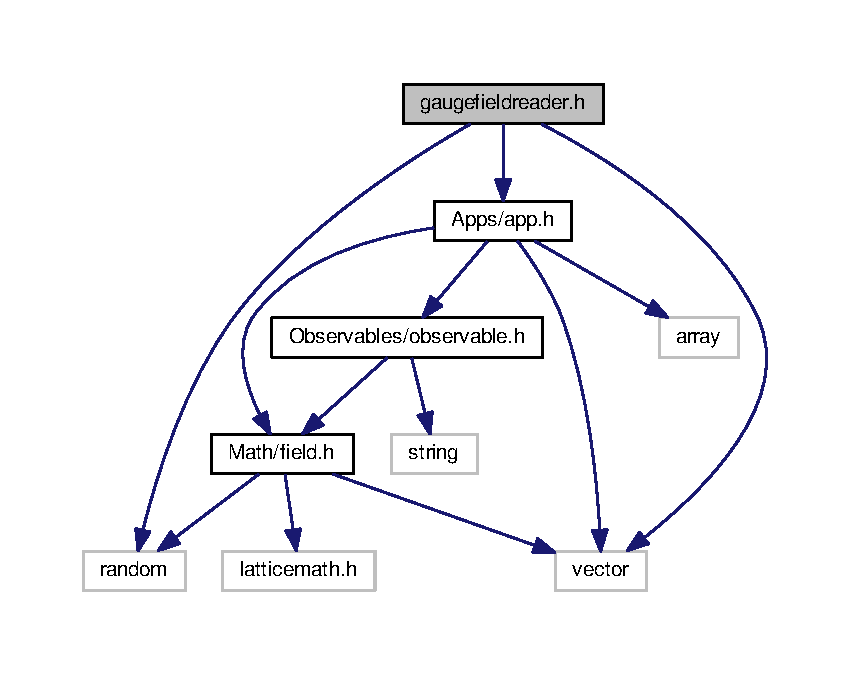
\includegraphics[width=350pt]{db/d9b/gaugefieldreader_8h__incl}
\end{center}
\end{figure}
This graph shows which files directly or indirectly include this file\+:\nopagebreak
\begin{figure}[H]
\begin{center}
\leavevmode
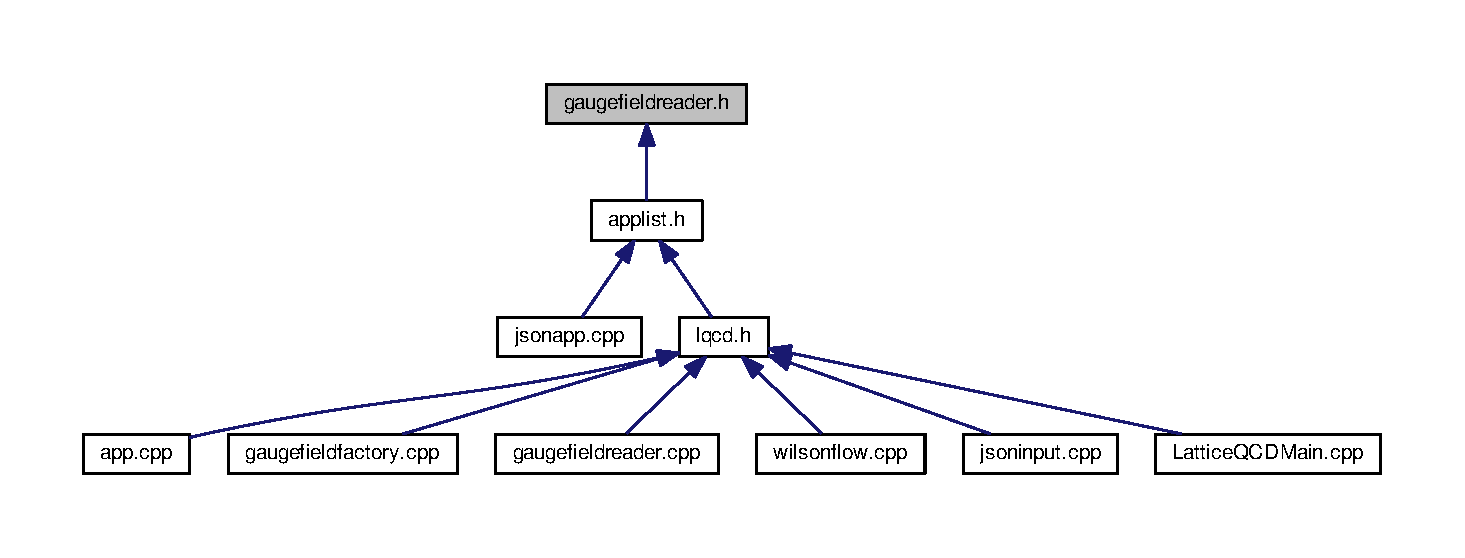
\includegraphics[width=350pt]{d4/d10/gaugefieldreader_8h__dep__incl}
\end{center}
\end{figure}
\subsection*{Classes}
\begin{DoxyCompactItemize}
\item 
class \hyperlink{classGaugeFieldReader}{Gauge\+Field\+Reader}
\begin{DoxyCompactList}\small\item\em Implementation of the \hyperlink{classGaugeFieldReader}{Gauge\+Field\+Reader} \hyperlink{classApp}{App} class. \end{DoxyCompactList}\end{DoxyCompactItemize}


\subsection{Detailed Description}
Contains the definition of the \hyperlink{classGaugeFieldReader}{Gauge\+Field\+Reader} \hyperlink{classApp}{App} derived class. 

\begin{DoxyAuthor}{Author}
Giovanni Pederiva 
\end{DoxyAuthor}
\begin{DoxyVersion}{Version}
1.\+0 
\end{DoxyVersion}
\begin{DoxyDate}{Date}
2017-\/2018 
\end{DoxyDate}
\begin{DoxyCopyright}{Copyright}
M\+IT License. 
\end{DoxyCopyright}

\hypertarget{inputconf_8cpp}{}\section{inputconf.\+cpp File Reference}
\label{inputconf_8cpp}\index{inputconf.\+cpp@{inputconf.\+cpp}}


Utilities for opening and reading gauge field configurations from disk in parallel.  


{\ttfamily \#include \char`\"{}Utils/clusterspecifier.\+h\char`\"{}}\\*
{\ttfamily \#include $<$mpi/mpi.\+h$>$}\\*
{\ttfamily \#include $<$cstdio$>$}\\*
{\ttfamily \#include $<$algorithm$>$}\\*
{\ttfamily \#include $<$boost/filesystem.\+hpp$>$}\\*
{\ttfamily \#include \char`\"{}Input\+Output/inputconf.\+h\char`\"{}}\\*
{\ttfamily \#include \char`\"{}Math/lattice.\+h\char`\"{}}\\*
{\ttfamily \#include \char`\"{}Parallel\+Tools/parallel.\+h\char`\"{}}\\*
Include dependency graph for inputconf.\+cpp\+:\nopagebreak
\begin{figure}[H]
\begin{center}
\leavevmode
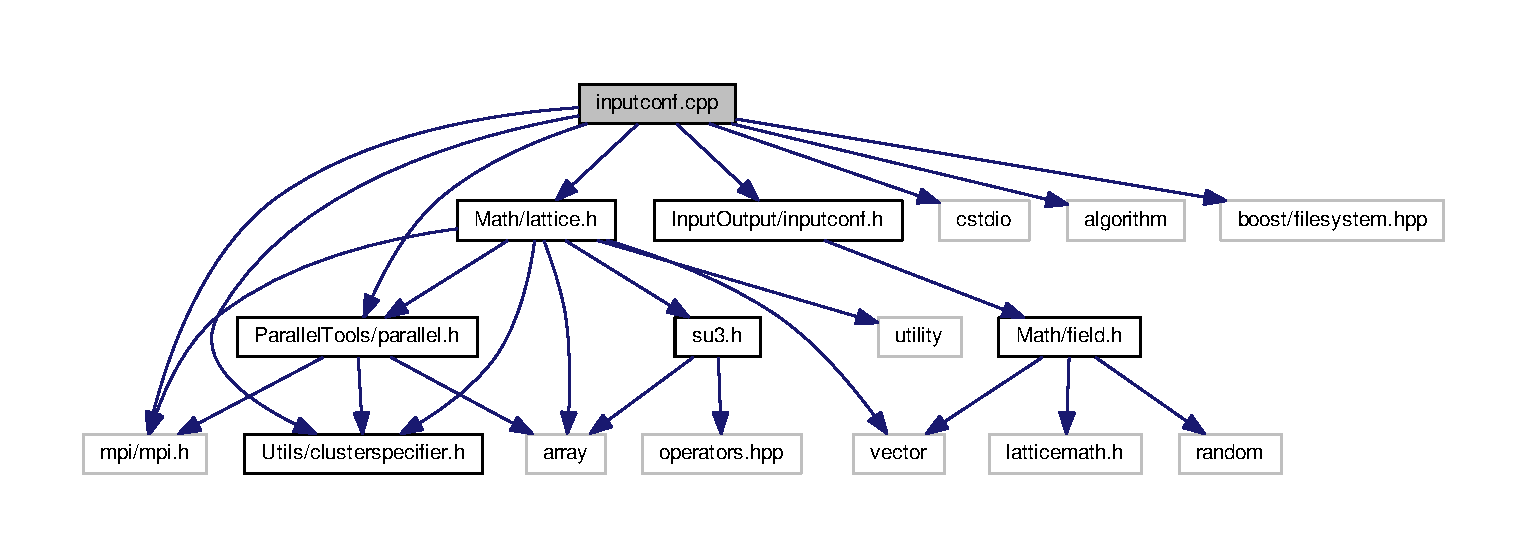
\includegraphics[width=350pt]{d1/dbe/inputconf_8cpp__incl}
\end{center}
\end{figure}
\subsection*{Functions}
\begin{DoxyCompactItemize}
\item 
double \hyperlink{inputconf_8cpp_aee292d5093340ed121095bbc184064eb}{Lattice\+I\+O\+::\+Reverse\+Float} (const double in\+Float)
\begin{DoxyCompactList}\small\item\em changes the endianess of a float variable \end{DoxyCompactList}\item 
double \hyperlink{inputconf_8cpp_a4f07f840c6b7a7e360c37d966e0294e6}{Lattice\+I\+O\+::\+Reverse\+Double} (const double in\+Double)
\begin{DoxyCompactList}\small\item\em changes the endianess of a double variable \end{DoxyCompactList}\end{DoxyCompactItemize}


\subsection{Detailed Description}
Utilities for opening and reading gauge field configurations from disk in parallel. 

\begin{DoxyAuthor}{Author}
Giovanni Pederiva 
\end{DoxyAuthor}
\begin{DoxyVersion}{Version}
1.\+0 
\end{DoxyVersion}
\begin{DoxyDate}{Date}
2017-\/2018 
\end{DoxyDate}
\begin{DoxyCopyright}{Copyright}
M\+IT License. 
\end{DoxyCopyright}


\subsection{Function Documentation}
\index{inputconf.\+cpp@{inputconf.\+cpp}!Reverse\+Double@{Reverse\+Double}}
\index{Reverse\+Double@{Reverse\+Double}!inputconf.\+cpp@{inputconf.\+cpp}}
\subsubsection[{\texorpdfstring{Reverse\+Double(const double in\+Double)}{ReverseDouble(const double inDouble)}}]{\setlength{\rightskip}{0pt plus 5cm}double Lattice\+I\+O\+::\+Reverse\+Double (
\begin{DoxyParamCaption}
\item[{const double}]{in\+Double}
\end{DoxyParamCaption}
)}\hypertarget{inputconf_8cpp_file_a4f07f840c6b7a7e360c37d966e0294e6}{}\label{inputconf_8cpp_file_a4f07f840c6b7a7e360c37d966e0294e6}


changes the endianess of a double variable 


\begin{DoxyParams}{Parameters}
{\em in\+Float} & a double variable \\
\hline
\end{DoxyParams}


Definition at line 75 of file inputconf.\+cpp.

\index{inputconf.\+cpp@{inputconf.\+cpp}!Reverse\+Float@{Reverse\+Float}}
\index{Reverse\+Float@{Reverse\+Float}!inputconf.\+cpp@{inputconf.\+cpp}}
\subsubsection[{\texorpdfstring{Reverse\+Float(const double in\+Float)}{ReverseFloat(const double inFloat)}}]{\setlength{\rightskip}{0pt plus 5cm}double Lattice\+I\+O\+::\+Reverse\+Float (
\begin{DoxyParamCaption}
\item[{const double}]{in\+Float}
\end{DoxyParamCaption}
)}\hypertarget{inputconf_8cpp_file_aee292d5093340ed121095bbc184064eb}{}\label{inputconf_8cpp_file_aee292d5093340ed121095bbc184064eb}


changes the endianess of a float variable 


\begin{DoxyParams}{Parameters}
{\em in\+Float} & a float variable \\
\hline
\end{DoxyParams}


Definition at line 54 of file inputconf.\+cpp.


\hypertarget{inputconf_8h}{}\section{inputconf.\+h File Reference}
\label{inputconf_8h}\index{inputconf.\+h@{inputconf.\+h}}


Contains classes for reading lattices from binary files.  


{\ttfamily \#include \char`\"{}Math/field.\+h\char`\"{}}\\*
Include dependency graph for inputconf.\+h\+:\nopagebreak
\begin{figure}[H]
\begin{center}
\leavevmode
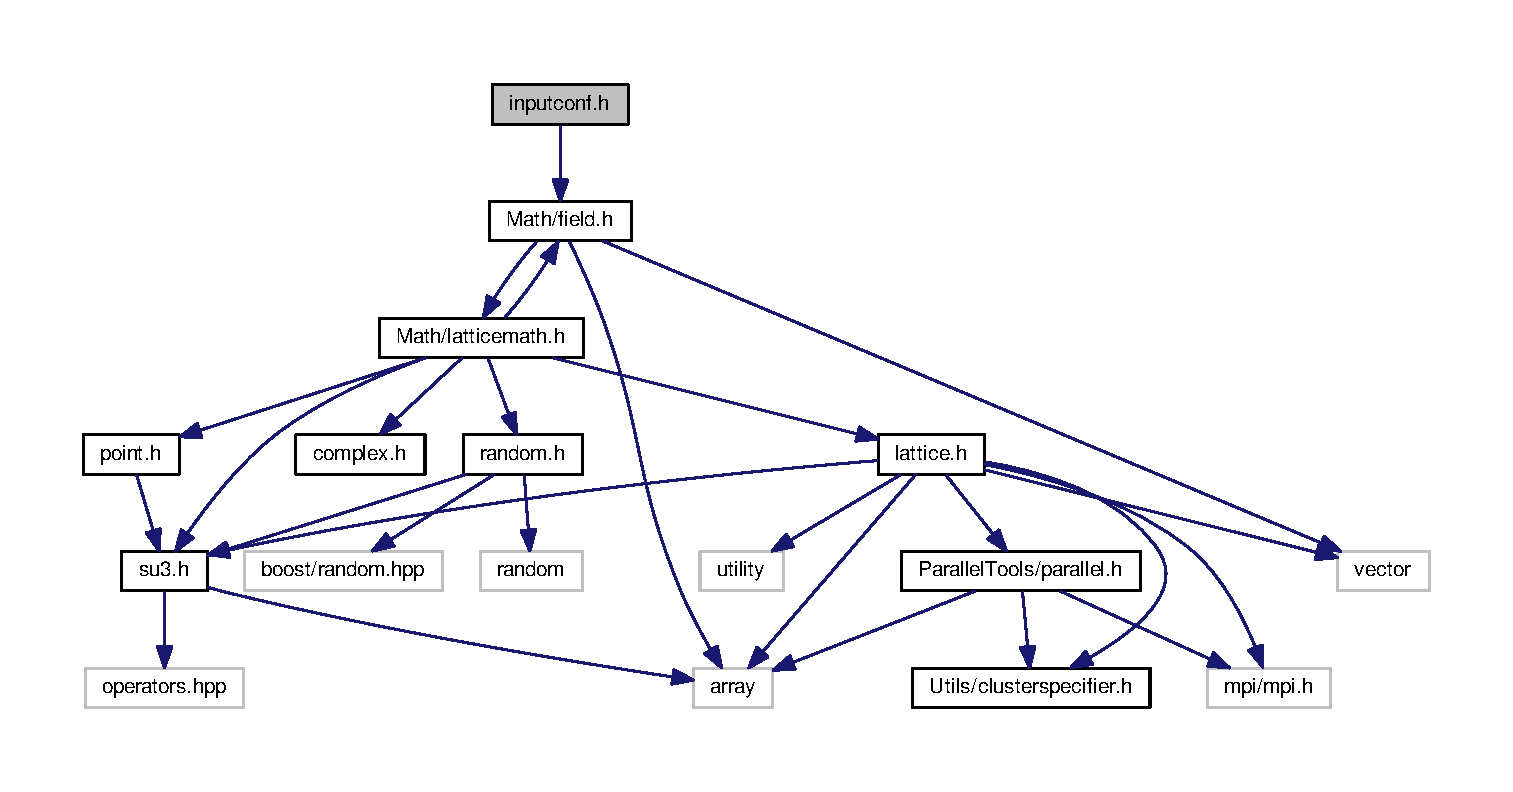
\includegraphics[width=350pt]{d0/d5b/inputconf_8h__incl}
\end{center}
\end{figure}
This graph shows which files directly or indirectly include this file\+:\nopagebreak
\begin{figure}[H]
\begin{center}
\leavevmode
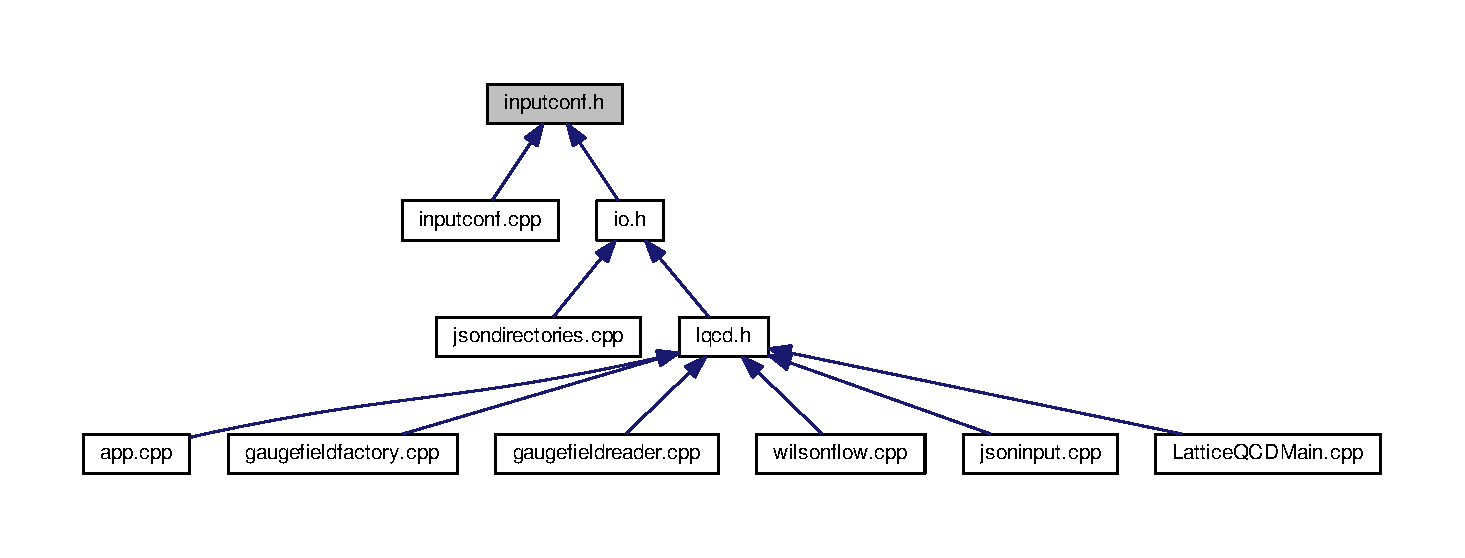
\includegraphics[width=350pt]{d9/d3e/inputconf_8h__dep__incl}
\end{center}
\end{figure}
\subsection*{Classes}
\begin{DoxyCompactItemize}
\item 
class \hyperlink{classLatticeIO_1_1InputConf}{Lattice\+I\+O\+::\+Input\+Conf}
\begin{DoxyCompactList}\small\item\em Class for reding lattices from binary files. \end{DoxyCompactList}\end{DoxyCompactItemize}


\subsection{Detailed Description}
Contains classes for reading lattices from binary files. 

\begin{DoxyAuthor}{Author}
Giovanni Pederiva 
\end{DoxyAuthor}
\begin{DoxyVersion}{Version}
1.\+0 
\end{DoxyVersion}
\begin{DoxyDate}{Date}
2017-\/2018 
\end{DoxyDate}
\begin{DoxyCopyright}{Copyright}
M\+IT License. 
\end{DoxyCopyright}

\hypertarget{io_8h}{}\section{io.\+h File Reference}
\label{io_8h}\index{io.\+h@{io.\+h}}


Main include file for input output related headers.  


{\ttfamily \#include \char`\"{}inputconf.\+h\char`\"{}}\\*
{\ttfamily \#include \char`\"{}outputconf.\+h\char`\"{}}\\*
{\ttfamily \#include \char`\"{}outputobs.\+h\char`\"{}}\\*
{\ttfamily \#include \char`\"{}outputterm.\+h\char`\"{}}\\*
{\ttfamily \#include \char`\"{}Json\+Input/jsoninput.\+h\char`\"{}}\\*
{\ttfamily \#include \char`\"{}Json\+Input/jsonitems.\+h\char`\"{}}\\*
Include dependency graph for io.\+h\+:\nopagebreak
\begin{figure}[H]
\begin{center}
\leavevmode
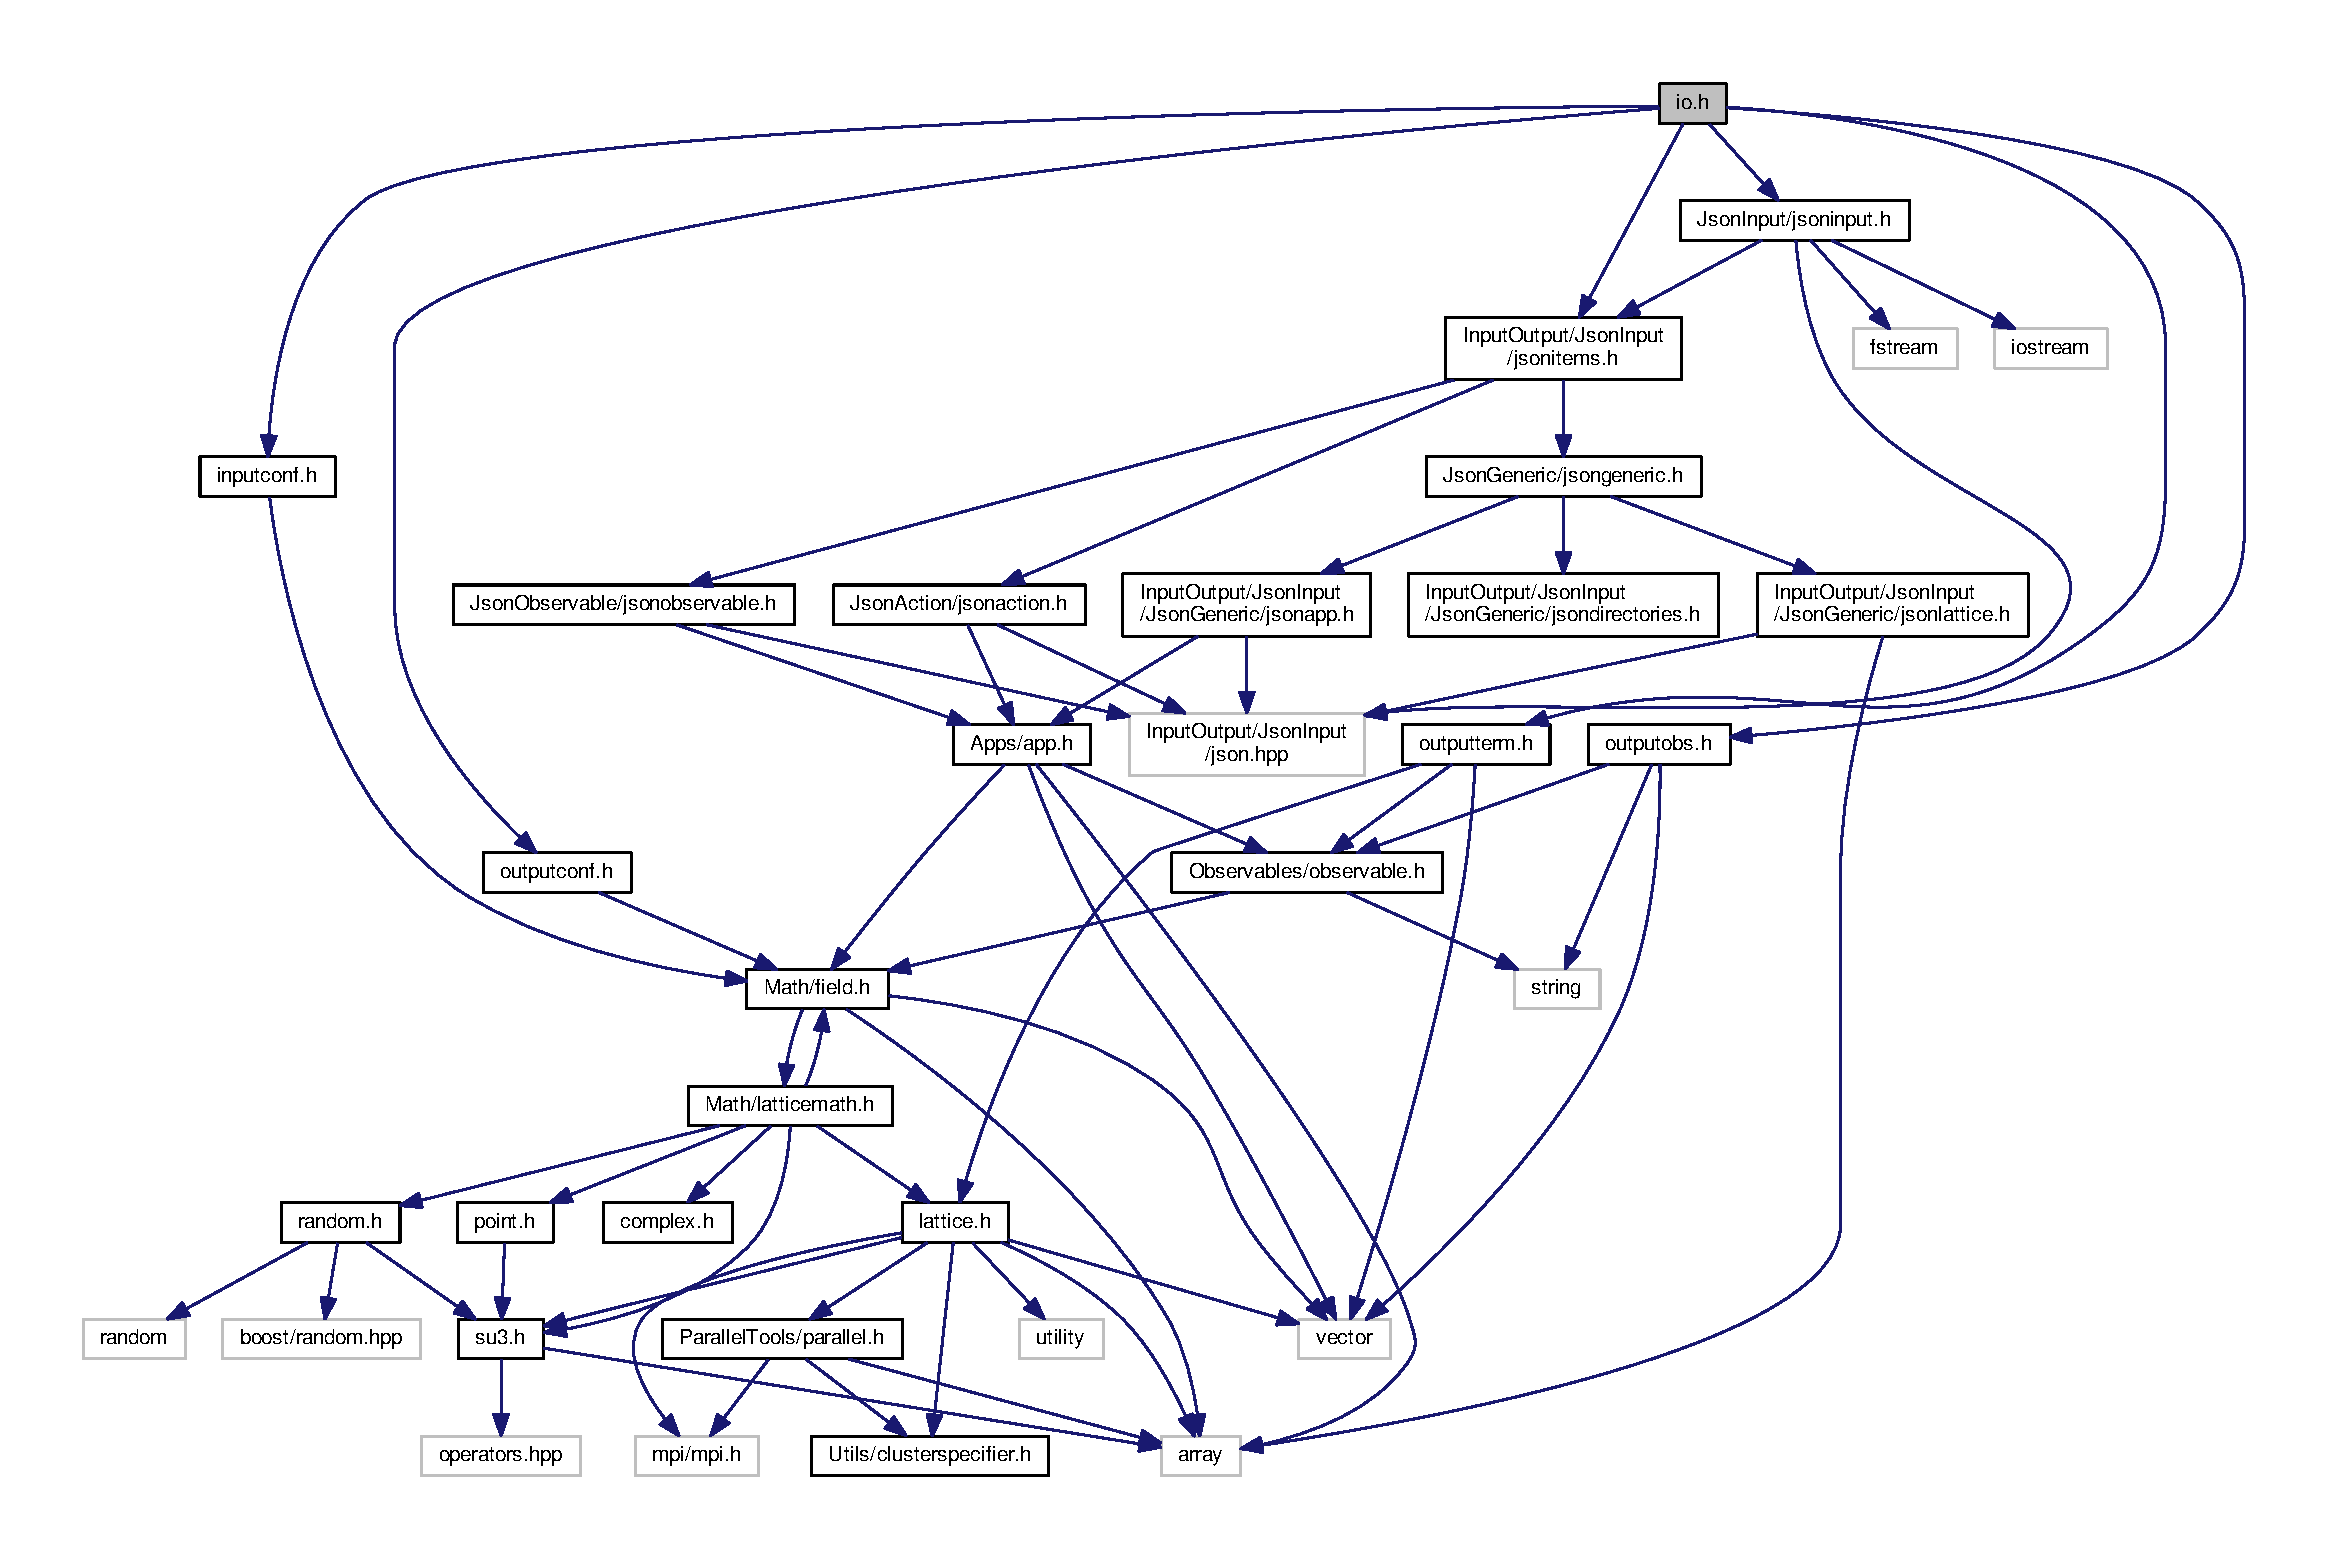
\includegraphics[width=350pt]{d8/da5/io_8h__incl}
\end{center}
\end{figure}
This graph shows which files directly or indirectly include this file\+:\nopagebreak
\begin{figure}[H]
\begin{center}
\leavevmode
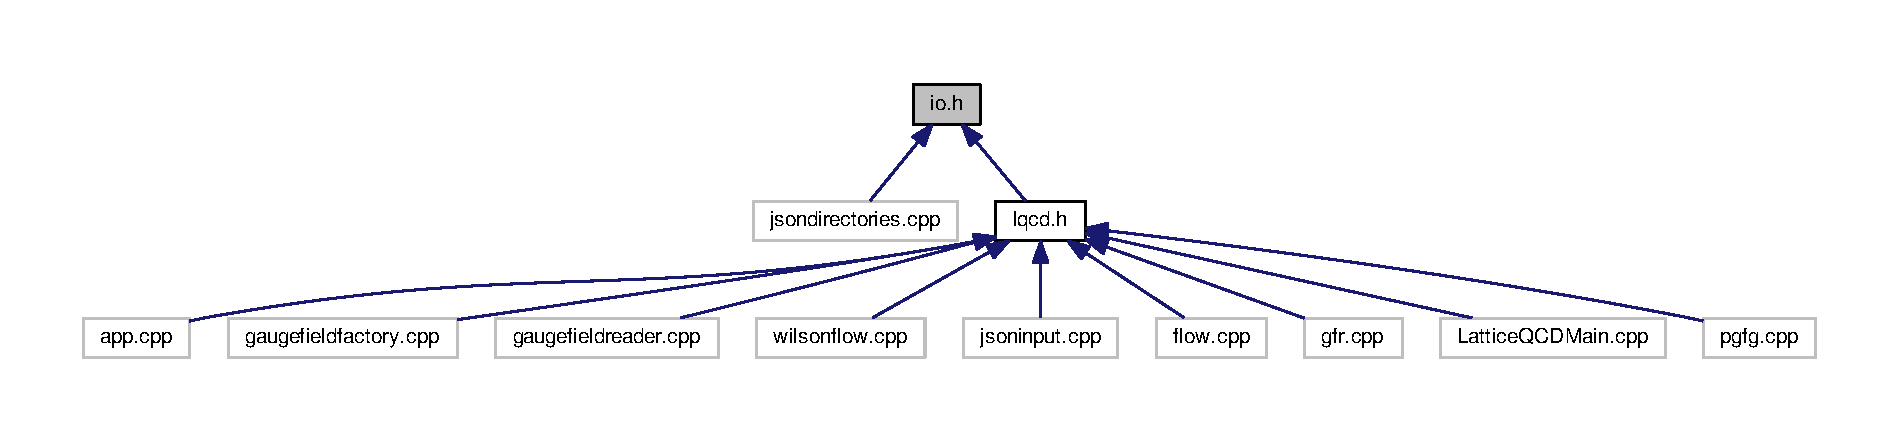
\includegraphics[width=350pt]{da/de4/io_8h__dep__incl}
\end{center}
\end{figure}


\subsection{Detailed Description}
Main include file for input output related headers. 

\begin{DoxyAuthor}{Author}
Giovanni Pederiva 
\end{DoxyAuthor}
\begin{DoxyVersion}{Version}
1.\+0 
\end{DoxyVersion}
\begin{DoxyDate}{Date}
2017-\/2018 
\end{DoxyDate}
\begin{DoxyCopyright}{Copyright}
M\+IT License.
\end{DoxyCopyright}
This file provides a simple access to all of the classes related to input output related routines. 
\hypertarget{lattice_8cpp}{}\section{lattice.\+cpp File Reference}
\label{lattice_8cpp}\index{lattice.\+cpp@{lattice.\+cpp}}


auxiliary functions of the \hyperlink{classLattice}{Lattice} class  


{\ttfamily \#include \char`\"{}Utils/clusterspecifier.\+h\char`\"{}}\\*
{\ttfamily \#include $<$mpi/mpi.\+h$>$}\\*
{\ttfamily \#include \char`\"{}Math/lattice.\+h\char`\"{}}\\*
{\ttfamily \#include \char`\"{}Math/point.\+h\char`\"{}}\\*
{\ttfamily \#include \char`\"{}Math/su3.\+h\char`\"{}}\\*
{\ttfamily \#include \char`\"{}Parallel\+Tools/parallel.\+h\char`\"{}}\\*
{\ttfamily \#include \char`\"{}Math/random.\+h\char`\"{}}\\*
{\ttfamily \#include $<$cstdio$>$}\\*
Include dependency graph for lattice.\+cpp\+:\nopagebreak
\begin{figure}[H]
\begin{center}
\leavevmode
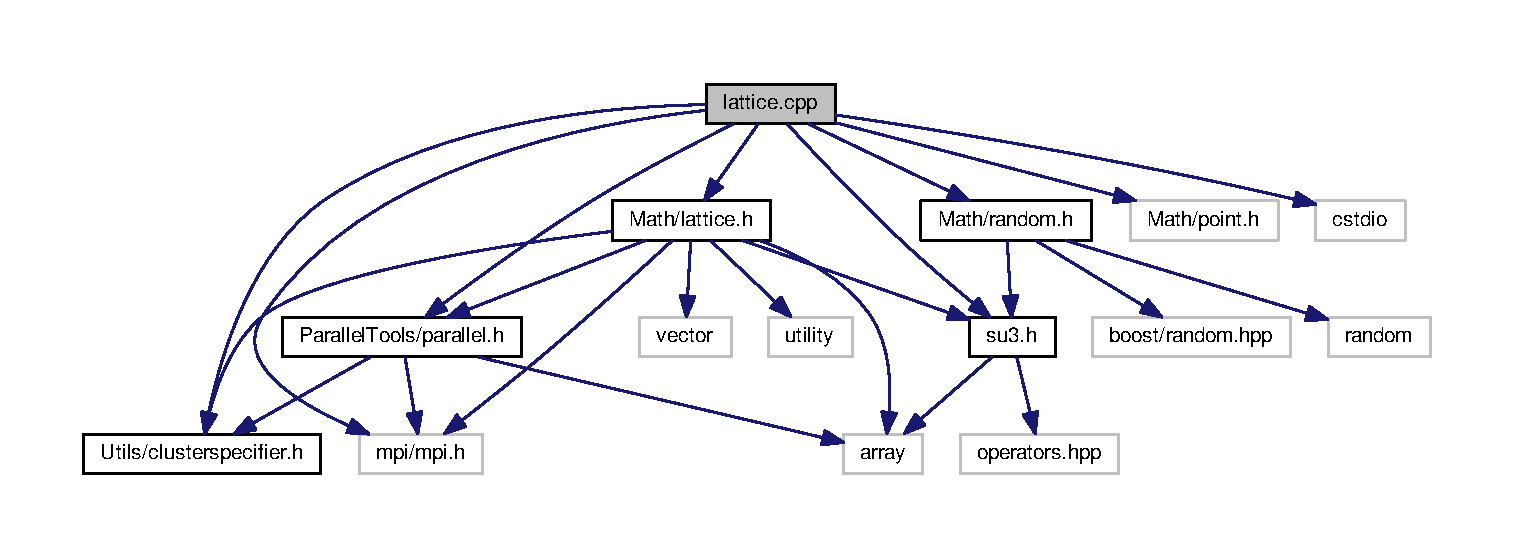
\includegraphics[width=350pt]{da/d81/lattice_8cpp__incl}
\end{center}
\end{figure}
\subsection*{Functions}
\begin{DoxyCompactItemize}
\item 
void \hyperlink{lattice_8cpp_a5def93dbbae6cc4897e9b0db15fbed86}{set\+Lattice\+Imag\+Identity\+Value} (\hyperlink{classLattice}{Lattice}$<$ \hyperlink{structSU3}{S\+U3} $>$ \&su3lat, const \hyperlink{classLattice}{Lattice}$<$ double $>$ \&lat)\hypertarget{lattice_8cpp_a5def93dbbae6cc4897e9b0db15fbed86}{}\label{lattice_8cpp_a5def93dbbae6cc4897e9b0db15fbed86}

\begin{DoxyCompactList}\small\item\em sets a lattice object to only diagonal matrices with complex values \end{DoxyCompactList}\item 
void {\bfseries set\+Lattice\+Imag\+Identity\+Value} (\hyperlink{classLattice}{Lattice}$<$ \hyperlink{structSU3}{S\+U3} $>$ \&su3lat, \hyperlink{classLattice}{Lattice}$<$ double $>$ \&\&lat)\hypertarget{lattice_8cpp_aa0b6c693b05ac17313064a8a419ca1e4}{}\label{lattice_8cpp_aa0b6c693b05ac17313064a8a419ca1e4}

\item 
void \hyperlink{lattice_8cpp_a8de3d17ae9ee16e9636b216f76c910e2}{set\+To\+Zero} (\hyperlink{classLattice}{Lattice}$<$ \hyperlink{structSU3}{S\+U3} $>$ \&su3lat)\hypertarget{lattice_8cpp_a8de3d17ae9ee16e9636b216f76c910e2}{}\label{lattice_8cpp_a8de3d17ae9ee16e9636b216f76c910e2}

\begin{DoxyCompactList}\small\item\em sets a lattice object to all zero matrices \end{DoxyCompactList}\item 
void \hyperlink{lattice_8cpp_ae4622adb92e4229ea06e6ec7ff60b973}{set\+To\+Identity} (\hyperlink{classLattice}{Lattice}$<$ \hyperlink{structSU3}{S\+U3} $>$ \&su3lat)\hypertarget{lattice_8cpp_ae4622adb92e4229ea06e6ec7ff60b973}{}\label{lattice_8cpp_ae4622adb92e4229ea06e6ec7ff60b973}

\begin{DoxyCompactList}\small\item\em sets a lattice object to all identity matrices \end{DoxyCompactList}\end{DoxyCompactItemize}


\subsection{Detailed Description}
auxiliary functions of the \hyperlink{classLattice}{Lattice} class 

\begin{DoxyAuthor}{Author}
Giovanni Pederiva 
\end{DoxyAuthor}
\begin{DoxyVersion}{Version}
1.\+0 
\end{DoxyVersion}
\begin{DoxyDate}{Date}
2017-\/2018 
\end{DoxyDate}
\begin{DoxyCopyright}{Copyright}
M\+IT License. 
\end{DoxyCopyright}

\hypertarget{lattice_8h}{}\section{lattice.\+h File Reference}
\label{lattice_8h}\index{lattice.\+h@{lattice.\+h}}


Contains the definition of the \hyperlink{classLattice}{Lattice} class.  


{\ttfamily \#include $<$vector$>$}\\*
{\ttfamily \#include $<$array$>$}\\*
{\ttfamily \#include $<$utility$>$}\\*
{\ttfamily \#include \char`\"{}su3.\+h\char`\"{}}\\*
{\ttfamily \#include \char`\"{}Utils/clusterspecifier.\+h\char`\"{}}\\*
{\ttfamily \#include $<$mpi/mpi.\+h$>$}\\*
{\ttfamily \#include \char`\"{}Parallel\+Tools/parallel.\+h\char`\"{}}\\*
Include dependency graph for lattice.\+h\+:
% FIG 0
This graph shows which files directly or indirectly include this file\+:
% FIG 1
\subsection*{Classes}
\begin{DoxyCompactItemize}
\item 
class \hyperlink{classLattice}{Lattice$<$ T $>$}
\begin{DoxyCompactList}\small\item\em Template class to store an array with 4 dimensional indices of a given datatype. Includes functionalities for parallel shifts. \end{DoxyCompactList}\end{DoxyCompactItemize}
\subsection*{Functions}
\begin{DoxyCompactItemize}
\item 
{\footnotesize template$<$typename T $>$ }\\\hyperlink{classLattice}{Lattice}$<$ T $>$ {\bfseries adj} (const \hyperlink{classLattice}{Lattice}$<$ T $>$ \&base)\hypertarget{lattice_8h_a05afa4123548656b402f62ccc413ab1d}{}\label{lattice_8h_a05afa4123548656b402f62ccc413ab1d}

\item 
{\footnotesize template$<$typename T $>$ }\\\hyperlink{classLattice}{Lattice}$<$ T $>$ {\bfseries adj} (\hyperlink{classLattice}{Lattice}$<$ T $>$ \&\&base)\hypertarget{lattice_8h_a383a84b4aee2453591a97e39cbc36570}{}\label{lattice_8h_a383a84b4aee2453591a97e39cbc36570}

\item 
{\footnotesize template$<$typename T $>$ }\\\hyperlink{classLattice}{Lattice}$<$ T $>$ {\bfseries exp} (const \hyperlink{classLattice}{Lattice}$<$ T $>$ \&base)\hypertarget{lattice_8h_ad197d2f28a71e181f799b36c215f02df}{}\label{lattice_8h_ad197d2f28a71e181f799b36c215f02df}

\item 
{\footnotesize template$<$typename T $>$ }\\\hyperlink{classLattice}{Lattice}$<$ T $>$ {\bfseries exp} (\hyperlink{classLattice}{Lattice}$<$ T $>$ \&\&base)\hypertarget{lattice_8h_a6389116ee142f144212ee764720d60b4}{}\label{lattice_8h_a6389116ee142f144212ee764720d60b4}

\item 
{\footnotesize template$<$typename T $>$ }\\T {\bfseries sum} (\hyperlink{classLattice}{Lattice}$<$ T $>$ \&base)\hypertarget{lattice_8h_a658434187e97cbc38659bae69ac2131e}{}\label{lattice_8h_a658434187e97cbc38659bae69ac2131e}

\item 
{\footnotesize template$<$$>$ }\\\hyperlink{structSU3}{S\+U3} {\bfseries sum} (\hyperlink{classLattice}{Lattice}$<$ \hyperlink{structSU3}{S\+U3} $>$ \&base)\hypertarget{lattice_8h_ae78399547c90209cf63a98a56b18e619}{}\label{lattice_8h_ae78399547c90209cf63a98a56b18e619}

\item 
{\footnotesize template$<$typename T $>$ }\\T {\bfseries sum} (\hyperlink{classLattice}{Lattice}$<$ T $>$ \&\&base)\hypertarget{lattice_8h_a84d140ceb525bd2cf9c566a4201333c8}{}\label{lattice_8h_a84d140ceb525bd2cf9c566a4201333c8}

\item 
{\footnotesize template$<$$>$ }\\\hyperlink{structSU3}{S\+U3} {\bfseries sum} (\hyperlink{classLattice}{Lattice}$<$ \hyperlink{structSU3}{S\+U3} $>$ \&\&base)\hypertarget{lattice_8h_a552295d833798f00b9f9d6bfef792f7b}{}\label{lattice_8h_a552295d833798f00b9f9d6bfef792f7b}

\item 
\hyperlink{classLattice}{Lattice}$<$ double $>$ {\bfseries real\+Trace} (\hyperlink{classLattice}{Lattice}$<$ \hyperlink{structSU3}{S\+U3} $>$ \&base)\hypertarget{lattice_8h_a38dbd7db933da29717c74be8c130a1e3}{}\label{lattice_8h_a38dbd7db933da29717c74be8c130a1e3}

\item 
\hyperlink{classLattice}{Lattice}$<$ double $>$ {\bfseries imag\+Trace} (\hyperlink{classLattice}{Lattice}$<$ \hyperlink{structSU3}{S\+U3} $>$ \&base)\hypertarget{lattice_8h_ae6f1cb48b3c7370bcf9e55e4bbea61db}{}\label{lattice_8h_ae6f1cb48b3c7370bcf9e55e4bbea61db}

\item 
\hyperlink{classLattice}{Lattice}$<$ double $>$ {\bfseries real\+Trace} (\hyperlink{classLattice}{Lattice}$<$ \hyperlink{structSU3}{S\+U3} $>$ \&\&base)\hypertarget{lattice_8h_a7678e5c7fd0381d978218253a5fb31e9}{}\label{lattice_8h_a7678e5c7fd0381d978218253a5fb31e9}

\item 
\hyperlink{classLattice}{Lattice}$<$ double $>$ {\bfseries imag\+Trace} (\hyperlink{classLattice}{Lattice}$<$ \hyperlink{structSU3}{S\+U3} $>$ \&\&base)\hypertarget{lattice_8h_a7336d85e24e4f20b77ee191573161752}{}\label{lattice_8h_a7336d85e24e4f20b77ee191573161752}

\item 
void {\bfseries set\+Lattice\+Imag\+Identity\+Value} (\hyperlink{classLattice}{Lattice}$<$ \hyperlink{structSU3}{S\+U3} $>$ \&su3lat, const \hyperlink{classLattice}{Lattice}$<$ double $>$ \&lat)\hypertarget{lattice_8h_a5def93dbbae6cc4897e9b0db15fbed86}{}\label{lattice_8h_a5def93dbbae6cc4897e9b0db15fbed86}

\item 
void {\bfseries set\+Lattice\+Imag\+Identity\+Value} (\hyperlink{classLattice}{Lattice}$<$ \hyperlink{structSU3}{S\+U3} $>$ \&su3lat, \hyperlink{classLattice}{Lattice}$<$ double $>$ \&\&lat)\hypertarget{lattice_8h_aa0b6c693b05ac17313064a8a419ca1e4}{}\label{lattice_8h_aa0b6c693b05ac17313064a8a419ca1e4}

\item 
void {\bfseries set\+To\+Zero} (\hyperlink{classLattice}{Lattice}$<$ \hyperlink{structSU3}{S\+U3} $>$ \&su3lat)\hypertarget{lattice_8h_a8de3d17ae9ee16e9636b216f76c910e2}{}\label{lattice_8h_a8de3d17ae9ee16e9636b216f76c910e2}

\item 
void {\bfseries set\+To\+Identity} (\hyperlink{classLattice}{Lattice}$<$ \hyperlink{structSU3}{S\+U3} $>$ \&su3lat)\hypertarget{lattice_8h_ae4622adb92e4229ea06e6ec7ff60b973}{}\label{lattice_8h_ae4622adb92e4229ea06e6ec7ff60b973}

\item 
{\footnotesize template$<$typename T $>$ }\\\hyperlink{classLattice}{Lattice}$<$ T $>$ {\bfseries shift} (const \hyperlink{classLattice}{Lattice}$<$ T $>$ \&lat, int shift\+Dir, int shift\+Step)\hypertarget{lattice_8h_aa8e188fda775fc8142f9358f39f7e9ab}{}\label{lattice_8h_aa8e188fda775fc8142f9358f39f7e9ab}

\item 
{\footnotesize template$<$typename T $>$ }\\\hyperlink{classLattice}{Lattice}$<$ T $>$ {\bfseries shift} (\hyperlink{classLattice}{Lattice}$<$ T $>$ \&\&lat, int shift\+Dir, int shift\+Step)\hypertarget{lattice_8h_adab76ff240514f99af5d7dabb3ee53c1}{}\label{lattice_8h_adab76ff240514f99af5d7dabb3ee53c1}

\end{DoxyCompactItemize}


\subsection{Detailed Description}
Contains the definition of the \hyperlink{classLattice}{Lattice} class. 

\begin{DoxyAuthor}{Author}
Giovanni Pederiva 
\end{DoxyAuthor}
\begin{DoxyVersion}{Version}
1.\+0 
\end{DoxyVersion}
\begin{DoxyDate}{Date}
2017-\/2018 
\end{DoxyDate}
\begin{DoxyCopyright}{Copyright}
M\+IT License. 
\end{DoxyCopyright}

\hypertarget{LatticeQCDMain_8cpp}{}\section{Lattice\+Q\+C\+D\+Main.\+cpp File Reference}
\label{LatticeQCDMain_8cpp}\index{Lattice\+Q\+C\+D\+Main.\+cpp@{Lattice\+Q\+C\+D\+Main.\+cpp}}


Main function of the program.  


{\ttfamily \#include $<$cstdio$>$}\\*
{\ttfamily \#include $<$chrono$>$}\\*
{\ttfamily \#include \char`\"{}lqcd.\+h\char`\"{}}\\*
Include dependency graph for Lattice\+Q\+C\+D\+Main.\+cpp\+:\nopagebreak
\begin{figure}[H]
\begin{center}
\leavevmode
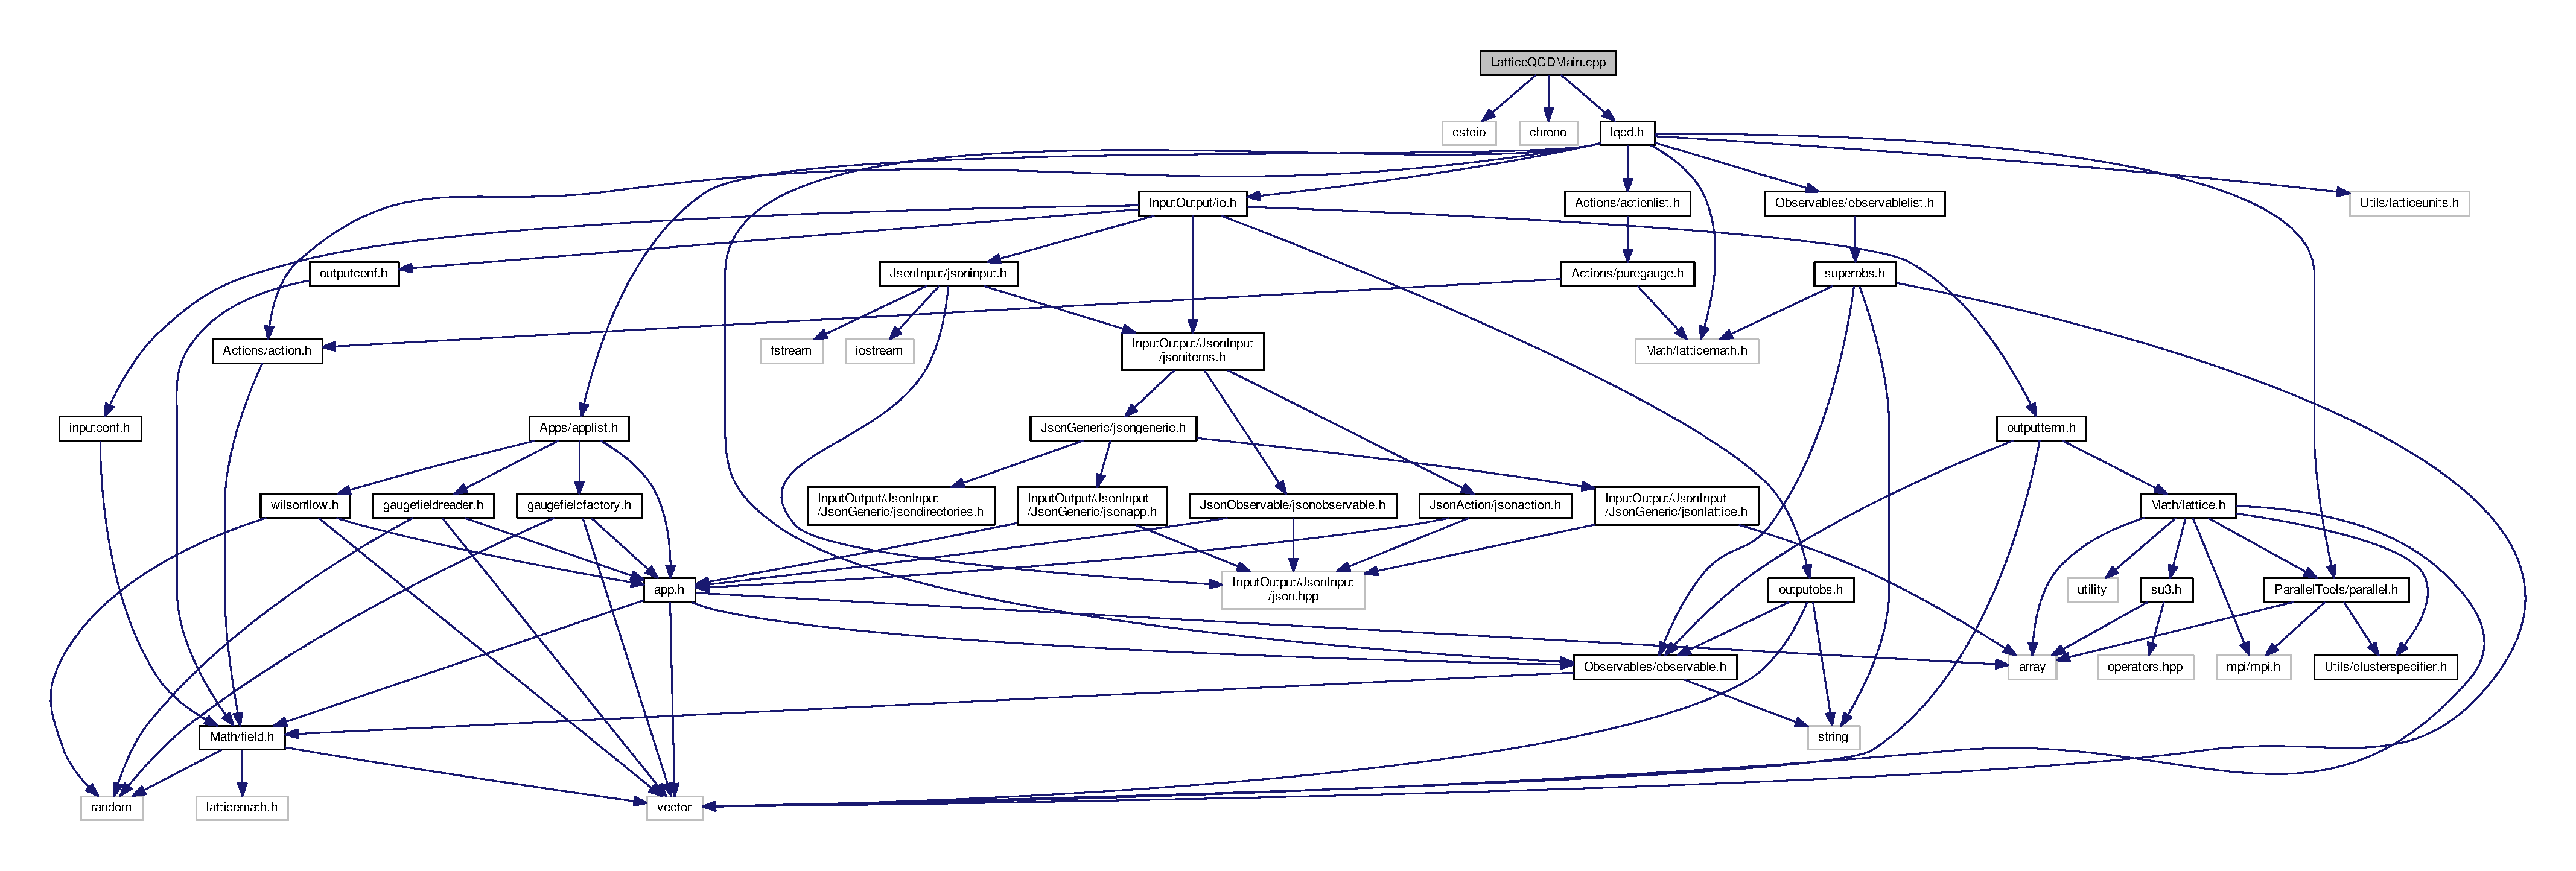
\includegraphics[width=350pt]{d7/d7e/LatticeQCDMain_8cpp__incl}
\end{center}
\end{figure}
\subsection*{Functions}
\begin{DoxyCompactItemize}
\item 
int {\bfseries main} (int argn, char $\ast$argv\mbox{[}$\,$\mbox{]})\hypertarget{LatticeQCDMain_8cpp_a31702bdafbf80639ac544c04a6733f52}{}\label{LatticeQCDMain_8cpp_a31702bdafbf80639ac544c04a6733f52}

\end{DoxyCompactItemize}


\subsection{Detailed Description}
Main function of the program. 

\begin{DoxyAuthor}{Author}
Giovanni Pederiva 
\end{DoxyAuthor}
\begin{DoxyVersion}{Version}
1.\+0 
\end{DoxyVersion}
\begin{DoxyDate}{Date}
2017-\/2018 
\end{DoxyDate}
\begin{DoxyCopyright}{Copyright}
M\+IT License. 
\end{DoxyCopyright}

\hypertarget{lqcd_8h}{}\section{lqcd.\+h File Reference}
\label{lqcd_8h}\index{lqcd.\+h@{lqcd.\+h}}


Main include file for all headers.  


{\ttfamily \#include \char`\"{}Actions/action.\+h\char`\"{}}\\*
{\ttfamily \#include \char`\"{}Actions/actionlist.\+h\char`\"{}}\\*
{\ttfamily \#include \char`\"{}Apps/applist.\+h\char`\"{}}\\*
{\ttfamily \#include \char`\"{}Input\+Output/io.\+h\char`\"{}}\\*
{\ttfamily \#include \char`\"{}Math/latticemath.\+h\char`\"{}}\\*
{\ttfamily \#include \char`\"{}Observables/observable.\+h\char`\"{}}\\*
{\ttfamily \#include \char`\"{}Observables/observablelist.\+h\char`\"{}}\\*
{\ttfamily \#include \char`\"{}Parallel\+Tools/parallel.\+h\char`\"{}}\\*
{\ttfamily \#include \char`\"{}Utils/latticeunits.\+h\char`\"{}}\\*
Include dependency graph for lqcd.\+h\+:
\nopagebreak
\begin{figure}[H]
\begin{center}
\leavevmode
\includegraphics[width=350pt]{dd/d16/lqcd_8h__incl}
\end{center}
\end{figure}
This graph shows which files directly or indirectly include this file\+:\nopagebreak
\begin{figure}[H]
\begin{center}
\leavevmode
\includegraphics[width=350pt]{df/d23/lqcd_8h__dep__incl}
\end{center}
\end{figure}


\subsection{Detailed Description}
Main include file for all headers. 

\begin{DoxyAuthor}{Author}
Giovanni Pederiva 
\end{DoxyAuthor}
\begin{DoxyVersion}{Version}
1.\+0 
\end{DoxyVersion}
\begin{DoxyDate}{Date}
2017-\/2018 
\end{DoxyDate}
\begin{DoxyCopyright}{Copyright}
M\+IT License.
\end{DoxyCopyright}
This file provides a simple access to all of the classes defined in the project. Includes all actions, apps, observables as well as base objects. 
\hypertarget{observable_8cpp}{}\section{observable.\+cpp File Reference}
\label{observable_8cpp}\index{observable.\+cpp@{observable.\+cpp}}


Base definition of the \hyperlink{classObservable}{Observable} prototype class.  


{\ttfamily \#include \char`\"{}Utils/clusterspecifier.\+h\char`\"{}}\\*
{\ttfamily \#include $<$mpi/mpi.\+h$>$}\\*
{\ttfamily \#include \char`\"{}Observables/observable.\+h\char`\"{}}\\*
{\ttfamily \#include \char`\"{}Math/lattice.\+h\char`\"{}}\\*
{\ttfamily \#include \char`\"{}Parallel\+Tools/parallel.\+h\char`\"{}}\\*
Include dependency graph for observable.\+cpp\+:\nopagebreak
\begin{figure}[H]
\begin{center}
\leavevmode
\includegraphics[width=350pt]{df/d78/observable_8cpp__incl}
\end{center}
\end{figure}


\subsection{Detailed Description}
Base definition of the \hyperlink{classObservable}{Observable} prototype class. 

\begin{DoxyAuthor}{Author}
Giovanni Pederiva 
\end{DoxyAuthor}
\begin{DoxyVersion}{Version}
1.\+0 
\end{DoxyVersion}
\begin{DoxyDate}{Date}
2017-\/2018 
\end{DoxyDate}
\begin{DoxyCopyright}{Copyright}
M\+IT License. 
\end{DoxyCopyright}

\hypertarget{observable_8h}{}\section{observable.\+h File Reference}
\label{observable_8h}\index{observable.\+h@{observable.\+h}}


Contains the definition of the \hyperlink{classObservable}{Observable} prototype.  


{\ttfamily \#include $<$string$>$}\\*
{\ttfamily \#include \char`\"{}Math/field.\+h\char`\"{}}\\*
Include dependency graph for observable.\+h\+:
% FIG 0
This graph shows which files directly or indirectly include this file\+:
% FIG 1
\subsection*{Classes}
\begin{DoxyCompactItemize}
\item 
class \hyperlink{classObservable}{Observable}
\begin{DoxyCompactList}\small\item\em Prototype for the \hyperlink{classObservable}{Observable} class group. \end{DoxyCompactList}\end{DoxyCompactItemize}


\subsection{Detailed Description}
Contains the definition of the \hyperlink{classObservable}{Observable} prototype. 

\begin{DoxyAuthor}{Author}
Giovanni Pederiva 
\end{DoxyAuthor}
\begin{DoxyVersion}{Version}
1.\+0 
\end{DoxyVersion}
\begin{DoxyDate}{Date}
2017-\/2018 
\end{DoxyDate}
\begin{DoxyCopyright}{Copyright}
M\+IT License. 
\end{DoxyCopyright}

\hypertarget{observablelist_8h}{}\section{observablelist.\+h File Reference}
\label{observablelist_8h}\index{observablelist.\+h@{observablelist.\+h}}


Main include file for \hyperlink{classObservable}{Observable} derived classes.  


{\ttfamily \#include \char`\"{}superobs.\+h\char`\"{}}\\*
Include dependency graph for observablelist.\+h\+:
% FIG 0
This graph shows which files directly or indirectly include this file\+:
% FIG 1


\subsection{Detailed Description}
Main include file for \hyperlink{classObservable}{Observable} derived classes. 

\begin{DoxyAuthor}{Author}
Giovanni Pederiva 
\end{DoxyAuthor}
\begin{DoxyVersion}{Version}
1.\+0 
\end{DoxyVersion}
\begin{DoxyDate}{Date}
2017-\/2018 
\end{DoxyDate}
\begin{DoxyCopyright}{Copyright}
M\+IT License.
\end{DoxyCopyright}
This file provides a simple access to all of the classes that implement the \hyperlink{classObservable}{Observable} type 
\hypertarget{outputconf_8cpp}{}\section{outputconf.\+cpp File Reference}
\label{outputconf_8cpp}\index{outputconf.\+cpp@{outputconf.\+cpp}}


Utilities for writing and saving gauge field configurations from disk in parallel.  


{\ttfamily \#include $<$boost/filesystem.\+hpp$>$}\\*
{\ttfamily \#include \char`\"{}Utils/clusterspecifier.\+h\char`\"{}}\\*
{\ttfamily \#include $<$mpi/mpi.\+h$>$}\\*
{\ttfamily \#include $<$cstdio$>$}\\*
{\ttfamily \#include \char`\"{}Input\+Output/outputconf.\+h\char`\"{}}\\*
{\ttfamily \#include \char`\"{}Math/lattice.\+h\char`\"{}}\\*
{\ttfamily \#include \char`\"{}Parallel\+Tools/parallel.\+h\char`\"{}}\\*
Include dependency graph for outputconf.\+cpp\+:\nopagebreak
\begin{figure}[H]
\begin{center}
\leavevmode
\includegraphics[width=350pt]{de/da4/outputconf_8cpp__incl}
\end{center}
\end{figure}


\subsection{Detailed Description}
Utilities for writing and saving gauge field configurations from disk in parallel. 

\begin{DoxyAuthor}{Author}
Giovanni Pederiva 
\end{DoxyAuthor}
\begin{DoxyVersion}{Version}
1.\+0 
\end{DoxyVersion}
\begin{DoxyDate}{Date}
2017-\/2018 
\end{DoxyDate}
\begin{DoxyCopyright}{Copyright}
M\+IT License. 
\end{DoxyCopyright}

\hypertarget{outputconf_8h}{}\section{outputconf.\+h File Reference}
\label{outputconf_8h}\index{outputconf.\+h@{outputconf.\+h}}


Contains classes for saving lattices to binary files.  


{\ttfamily \#include \char`\"{}Math/field.\+h\char`\"{}}\\*
Include dependency graph for outputconf.\+h\+:\nopagebreak
\begin{figure}[H]
\begin{center}
\leavevmode
\includegraphics[width=350pt]{dd/d28/outputconf_8h__incl}
\end{center}
\end{figure}
This graph shows which files directly or indirectly include this file\+:\nopagebreak
\begin{figure}[H]
\begin{center}
\leavevmode
\includegraphics[width=350pt]{dc/dd1/outputconf_8h__dep__incl}
\end{center}
\end{figure}
\subsection*{Classes}
\begin{DoxyCompactItemize}
\item 
class \hyperlink{classLatticeIO_1_1OutputConf}{Lattice\+I\+O\+::\+Output\+Conf}
\begin{DoxyCompactList}\small\item\em Class for saving lattices to binary files. \end{DoxyCompactList}\end{DoxyCompactItemize}


\subsection{Detailed Description}
Contains classes for saving lattices to binary files. 

\begin{DoxyAuthor}{Author}
Giovanni Pederiva 
\end{DoxyAuthor}
\begin{DoxyVersion}{Version}
1.\+0 
\end{DoxyVersion}
\begin{DoxyDate}{Date}
2017-\/2018 
\end{DoxyDate}
\begin{DoxyCopyright}{Copyright}
M\+IT License.
\end{DoxyCopyright}
This file mainly serves the purpose of providing an interface for saving Gluon\+Field objects into binary format. 
\hypertarget{outputobs_8cpp}{}\section{outputobs.\+cpp File Reference}
\label{outputobs_8cpp}\index{outputobs.\+cpp@{outputobs.\+cpp}}


Utilities to write output files containing observables values.  


{\ttfamily \#include $<$cstdio$>$}\\*
{\ttfamily \#include $<$boost/filesystem.\+hpp$>$}\\*
{\ttfamily \#include \char`\"{}Observables/observable.\+h\char`\"{}}\\*
{\ttfamily \#include \char`\"{}Input\+Output/outputobs.\+h\char`\"{}}\\*
{\ttfamily \#include \char`\"{}Math/lattice.\+h\char`\"{}}\\*
{\ttfamily \#include \char`\"{}Parallel\+Tools/parallel.\+h\char`\"{}}\\*
Include dependency graph for outputobs.\+cpp\+:\nopagebreak
\begin{figure}[H]
\begin{center}
\leavevmode
\includegraphics[width=350pt]{d2/d97/outputobs_8cpp__incl}
\end{center}
\end{figure}


\subsection{Detailed Description}
Utilities to write output files containing observables values. 

\begin{DoxyAuthor}{Author}
Giovanni Pederiva 
\end{DoxyAuthor}
\begin{DoxyVersion}{Version}
1.\+0 
\end{DoxyVersion}
\begin{DoxyDate}{Date}
2017-\/2018 
\end{DoxyDate}
\begin{DoxyCopyright}{Copyright}
M\+IT License. 
\end{DoxyCopyright}

\hypertarget{outputobs_8h}{}\section{outputobs.\+h File Reference}
\label{outputobs_8h}\index{outputobs.\+h@{outputobs.\+h}}


Contains classes for output to file of observables values.  


{\ttfamily \#include $<$vector$>$}\\*
{\ttfamily \#include $<$string$>$}\\*
{\ttfamily \#include \char`\"{}Observables/observable.\+h\char`\"{}}\\*
Include dependency graph for outputobs.\+h\+:\nopagebreak
\begin{figure}[H]
\begin{center}
\leavevmode
\includegraphics[width=350pt]{da/daa/outputobs_8h__incl}
\end{center}
\end{figure}
This graph shows which files directly or indirectly include this file\+:\nopagebreak
\begin{figure}[H]
\begin{center}
\leavevmode
\includegraphics[width=350pt]{d6/d15/outputobs_8h__dep__incl}
\end{center}
\end{figure}
\subsection*{Classes}
\begin{DoxyCompactItemize}
\item 
class \hyperlink{classLatticeIO_1_1OutputObs}{Lattice\+I\+O\+::\+Output\+Obs}
\begin{DoxyCompactList}\small\item\em Class for output to file of observables values. \end{DoxyCompactList}\end{DoxyCompactItemize}


\subsection{Detailed Description}
Contains classes for output to file of observables values. 

\begin{DoxyAuthor}{Author}
Giovanni Pederiva 
\end{DoxyAuthor}
\begin{DoxyVersion}{Version}
1.\+0 
\end{DoxyVersion}
\begin{DoxyDate}{Date}
2017-\/2018 
\end{DoxyDate}
\begin{DoxyCopyright}{Copyright}
M\+IT License.
\end{DoxyCopyright}
This file defines the class needed to file the values of the observables at different steps in the execution. It handles through M\+PI the acces to files depending on rank. 
\hypertarget{outputterm_8cpp}{}\section{outputterm.\+cpp File Reference}
\label{outputterm_8cpp}\index{outputterm.\+cpp@{outputterm.\+cpp}}


Utilities to write output to terminal during execution.  


{\ttfamily \#include $<$cstdio$>$}\\*
{\ttfamily \#include \char`\"{}Input\+Output/outputterm.\+h\char`\"{}}\\*
{\ttfamily \#include \char`\"{}Math/lattice.\+h\char`\"{}}\\*
{\ttfamily \#include \char`\"{}Parallel\+Tools/parallel.\+h\char`\"{}}\\*
{\ttfamily \#include \char`\"{}Observables/observable.\+h\char`\"{}}\\*
Include dependency graph for outputterm.\+cpp\+:\nopagebreak
\begin{figure}[H]
\begin{center}
\leavevmode
\includegraphics[width=350pt]{d0/d39/outputterm_8cpp__incl}
\end{center}
\end{figure}


\subsection{Detailed Description}
Utilities to write output to terminal during execution. 

\begin{DoxyAuthor}{Author}
Giovanni Pederiva 
\end{DoxyAuthor}
\begin{DoxyVersion}{Version}
1.\+0 
\end{DoxyVersion}
\begin{DoxyDate}{Date}
2017-\/2018 
\end{DoxyDate}
\begin{DoxyCopyright}{Copyright}
M\+IT License. 
\end{DoxyCopyright}

\hypertarget{outputterm_8h}{}\section{outputterm.\+h File Reference}
\label{outputterm_8h}\index{outputterm.\+h@{outputterm.\+h}}


Contains classes for output to standard command line interface.  


{\ttfamily \#include $<$vector$>$}\\*
{\ttfamily \#include \char`\"{}Math/lattice.\+h\char`\"{}}\\*
{\ttfamily \#include \char`\"{}Observables/observable.\+h\char`\"{}}\\*
Include dependency graph for outputterm.\+h\+:\nopagebreak
\begin{figure}[H]
\begin{center}
\leavevmode
\includegraphics[width=350pt]{da/d4d/outputterm_8h__incl}
\end{center}
\end{figure}
This graph shows which files directly or indirectly include this file\+:\nopagebreak
\begin{figure}[H]
\begin{center}
\leavevmode
\includegraphics[width=350pt]{d8/d44/outputterm_8h__dep__incl}
\end{center}
\end{figure}
\subsection*{Classes}
\begin{DoxyCompactItemize}
\item 
class \hyperlink{classLatticeIO_1_1OutputTerm}{Lattice\+I\+O\+::\+Output\+Term}
\begin{DoxyCompactList}\small\item\em Class for standard output. \end{DoxyCompactList}\end{DoxyCompactItemize}


\subsection{Detailed Description}
Contains classes for output to standard command line interface. 

\begin{DoxyAuthor}{Author}
Giovanni Pederiva 
\end{DoxyAuthor}
\begin{DoxyVersion}{Version}
1.\+0 
\end{DoxyVersion}
\begin{DoxyDate}{Date}
2017-\/2018 
\end{DoxyDate}
\begin{DoxyCopyright}{Copyright}
M\+IT License.
\end{DoxyCopyright}
This file defines the class needed for ouputting to standard command line interface, handling the multiprocess nature of the code. Namely it only allows one processor to output any data, preventing the others from doing anything. 
\hypertarget{parallel_8cpp}{}\section{parallel.\+cpp File Reference}
\label{parallel_8cpp}\index{parallel.\+cpp@{parallel.\+cpp}}


static class \hyperlink{classParallel}{Parallel} definitions and tools for parallelization  


{\ttfamily \#include \char`\"{}Utils/clusterspecifier.\+h\char`\"{}}\\*
{\ttfamily \#include $<$mpi/mpi.\+h$>$}\\*
{\ttfamily \#include \char`\"{}Parallel\+Tools/parallel.\+h\char`\"{}}\\*
{\ttfamily \#include $<$array$>$}\\*
Include dependency graph for parallel.\+cpp\+:\nopagebreak
\begin{figure}[H]
\begin{center}
\leavevmode
\includegraphics[width=350pt]{d8/d4f/parallel_8cpp__incl}
\end{center}
\end{figure}


\subsection{Detailed Description}
static class \hyperlink{classParallel}{Parallel} definitions and tools for parallelization 

\begin{DoxyAuthor}{Author}
Giovanni Pederiva 
\end{DoxyAuthor}
\begin{DoxyVersion}{Version}
1.\+0 
\end{DoxyVersion}
\begin{DoxyDate}{Date}
2017-\/2018 
\end{DoxyDate}
\begin{DoxyCopyright}{Copyright}
M\+IT License. 
\end{DoxyCopyright}

\hypertarget{parallel_8h}{}\section{parallel.\+h File Reference}
\label{parallel_8h}\index{parallel.\+h@{parallel.\+h}}


Utilities for parallelization.  


{\ttfamily \#include \char`\"{}Utils/clusterspecifier.\+h\char`\"{}}\\*
{\ttfamily \#include $<$mpi/mpi.\+h$>$}\\*
{\ttfamily \#include $<$array$>$}\\*
Include dependency graph for parallel.\+h\+:
% FIG 0
This graph shows which files directly or indirectly include this file\+:
% FIG 1
\subsection*{Classes}
\begin{DoxyCompactItemize}
\item 
class \hyperlink{classParallel}{Parallel}
\begin{DoxyCompactList}\small\item\em Class to manage the parallelization scheme. \end{DoxyCompactList}\end{DoxyCompactItemize}


\subsection{Detailed Description}
Utilities for parallelization. 

\begin{DoxyAuthor}{Author}
Giovanni Pederiva 
\end{DoxyAuthor}
\begin{DoxyVersion}{Version}
1.\+0 
\end{DoxyVersion}
\begin{DoxyDate}{Date}
2017-\/2018 
\end{DoxyDate}
\begin{DoxyCopyright}{Copyright}
M\+IT License. 
\end{DoxyCopyright}

\hypertarget{plaquette_8cpp}{}\section{plaquette.\+cpp File Reference}
\label{plaquette_8cpp}\index{plaquette.\+cpp@{plaquette.\+cpp}}


Details of the plaquette observable class (old)  


{\ttfamily \#include \char`\"{}Observables/plaquette.\+h\char`\"{}}\\*
{\ttfamily \#include \char`\"{}Observables/observable.\+h\char`\"{}}\\*
{\ttfamily \#include \char`\"{}Math/su3.\+h\char`\"{}}\\*
{\ttfamily \#include \char`\"{}Parallel\+Tools/parallel.\+h\char`\"{}}\\*
{\ttfamily \#include \char`\"{}Math/lattice.\+h\char`\"{}}\\*
{\ttfamily \#include $<$cstdio$>$}\\*
{\ttfamily \#include $<$cmath$>$}\\*
{\ttfamily \#include $<$string$>$}\\*
{\ttfamily \#include $<$iostream$>$}\\*
Include dependency graph for plaquette.\+cpp\+:\nopagebreak
\begin{figure}[H]
\begin{center}
\leavevmode
\includegraphics[width=350pt]{dc/dbf/plaquette_8cpp__incl}
\end{center}
\end{figure}


\subsection{Detailed Description}
Details of the plaquette observable class (old) 

\begin{DoxyAuthor}{Author}
Giovanni Pederiva 
\end{DoxyAuthor}
\begin{DoxyVersion}{Version}
0.\+1 
\end{DoxyVersion}
\begin{DoxyDate}{Date}
2017-\/2018 
\end{DoxyDate}
\begin{DoxyCopyright}{Copyright}
M\+IT License. 
\end{DoxyCopyright}

\hypertarget{plaquette_8h}{}\section{plaquette.\+h File Reference}
\label{plaquette_8h}\index{plaquette.\+h@{plaquette.\+h}}


Contains the definition of the \hyperlink{classPlaquette}{Plaquette} observable.  


{\ttfamily \#include $<$vector$>$}\\*
{\ttfamily \#include $<$string$>$}\\*
{\ttfamily \#include \char`\"{}Observables/observable.\+h\char`\"{}}\\*
{\ttfamily \#include \char`\"{}Math/latticemath.\+h\char`\"{}}\\*
Include dependency graph for plaquette.\+h\+:\nopagebreak
\begin{figure}[H]
\begin{center}
\leavevmode
\includegraphics[width=350pt]{d4/d96/plaquette_8h__incl}
\end{center}
\end{figure}
This graph shows which files directly or indirectly include this file\+:\nopagebreak
\begin{figure}[H]
\begin{center}
\leavevmode
\includegraphics[width=155pt]{da/d15/plaquette_8h__dep__incl}
\end{center}
\end{figure}
\subsection*{Classes}
\begin{DoxyCompactItemize}
\item 
class \hyperlink{classPlaquette}{Plaquette}
\begin{DoxyCompactList}\small\item\em Implementation of the \hyperlink{classPlaquette}{Plaquette} operator class. \end{DoxyCompactList}\end{DoxyCompactItemize}


\subsection{Detailed Description}
Contains the definition of the \hyperlink{classPlaquette}{Plaquette} observable. 

\begin{DoxyAuthor}{Author}
Giovanni Pederiva 
\end{DoxyAuthor}
\begin{DoxyVersion}{Version}
0.\+1 
\end{DoxyVersion}
\begin{DoxyDate}{Date}
2017-\/2018 
\end{DoxyDate}
\begin{DoxyCopyright}{Copyright}
M\+IT License. 
\end{DoxyCopyright}

\hypertarget{puregauge_8cpp}{}\section{puregauge.\+cpp File Reference}
\label{puregauge_8cpp}\index{puregauge.\+cpp@{puregauge.\+cpp}}


Details of the \hyperlink{classPureGauge}{Pure\+Gauge} action class.  


{\ttfamily \#include $<$cstdio$>$}\\*
{\ttfamily \#include $<$cmath$>$}\\*
{\ttfamily \#include \char`\"{}Actions/puregauge.\+h\char`\"{}}\\*
{\ttfamily \#include \char`\"{}Math/latticemath.\+h\char`\"{}}\\*
{\ttfamily \#include \char`\"{}Utils/latticeunits.\+h\char`\"{}}\\*
{\ttfamily \#include \char`\"{}Parallel\+Tools/parallel.\+h\char`\"{}}\\*
{\ttfamily \#include \char`\"{}Utils/clusterspecifier.\+h\char`\"{}}\\*
{\ttfamily \#include $<$mpi/mpi.\+h$>$}\\*
Include dependency graph for puregauge.\+cpp\+:\nopagebreak
\begin{figure}[H]
\begin{center}
\leavevmode
\includegraphics[width=350pt]{de/d6b/puregauge_8cpp__incl}
\end{center}
\end{figure}


\subsection{Detailed Description}
Details of the \hyperlink{classPureGauge}{Pure\+Gauge} action class. 

\begin{DoxyAuthor}{Author}
Giovanni Pederiva 
\end{DoxyAuthor}
\begin{DoxyVersion}{Version}
1.\+0 
\end{DoxyVersion}
\begin{DoxyDate}{Date}
2017-\/2018 
\end{DoxyDate}
\begin{DoxyCopyright}{Copyright}
M\+IT License. 
\end{DoxyCopyright}

\hypertarget{puregauge_8h}{}\section{puregauge.\+h File Reference}
\label{puregauge_8h}\index{puregauge.\+h@{puregauge.\+h}}


Contains the definition of the \hyperlink{classPureGauge}{Pure\+Gauge} action derived class.  


{\ttfamily \#include \char`\"{}Actions/action.\+h\char`\"{}}\\*
{\ttfamily \#include \char`\"{}Math/latticemath.\+h\char`\"{}}\\*
Include dependency graph for puregauge.\+h\+:
% FIG 0
This graph shows which files directly or indirectly include this file\+:
% FIG 1
\subsection*{Classes}
\begin{DoxyCompactItemize}
\item 
class \hyperlink{classPureGauge}{Pure\+Gauge}
\begin{DoxyCompactList}\small\item\em Implementation of the \hyperlink{classPureGauge}{Pure\+Gauge} derived \hyperlink{classAction}{Action} class. \end{DoxyCompactList}\end{DoxyCompactItemize}


\subsection{Detailed Description}
Contains the definition of the \hyperlink{classPureGauge}{Pure\+Gauge} action derived class. 

\begin{DoxyAuthor}{Author}
Giovanni Pederiva 
\end{DoxyAuthor}
\begin{DoxyVersion}{Version}
1.\+0 
\end{DoxyVersion}
\begin{DoxyDate}{Date}
2017-\/2018 
\end{DoxyDate}
\begin{DoxyCopyright}{Copyright}
M\+IT License. 
\end{DoxyCopyright}

\hypertarget{random_8cpp}{}\section{random.\+cpp File Reference}
\label{random_8cpp}\index{random.\+cpp@{random.\+cpp}}


Definition of the static random number and R\+NG related functions.  


{\ttfamily \#include \char`\"{}Math/su3.\+h\char`\"{}}\\*
{\ttfamily \#include \char`\"{}Math/random.\+h\char`\"{}}\\*
{\ttfamily \#include \char`\"{}Math/complex.\+h\char`\"{}}\\*
{\ttfamily \#include $<$random$>$}\\*
{\ttfamily \#include $<$boost/random.\+hpp$>$}\\*
Include dependency graph for random.\+cpp\+:\nopagebreak
\begin{figure}[H]
\begin{center}
\leavevmode
\includegraphics[width=350pt]{df/d07/random_8cpp__incl}
\end{center}
\end{figure}


\subsection{Detailed Description}
Definition of the static random number and R\+NG related functions. 

\begin{DoxyAuthor}{Author}
Giovanni Pederiva 
\end{DoxyAuthor}
\begin{DoxyVersion}{Version}
1.\+0 
\end{DoxyVersion}
\begin{DoxyDate}{Date}
2017-\/2018 
\end{DoxyDate}
\begin{DoxyCopyright}{Copyright}
M\+IT License. 
\end{DoxyCopyright}

\hypertarget{random_8h}{}\section{random.\+h File Reference}
\label{random_8h}\index{random.\+h@{random.\+h}}


Contains the definition of the \hyperlink{classRandom}{Random} class.  


{\ttfamily \#include $<$random$>$}\\*
{\ttfamily \#include $<$boost/random.\+hpp$>$}\\*
{\ttfamily \#include \char`\"{}Math/su3.\+h\char`\"{}}\\*
Include dependency graph for random.\+h\+:\nopagebreak
\begin{figure}[H]
\begin{center}
\leavevmode
\includegraphics[width=350pt]{db/dfa/random_8h__incl}
\end{center}
\end{figure}
This graph shows which files directly or indirectly include this file\+:\nopagebreak
\begin{figure}[H]
\begin{center}
\leavevmode
\includegraphics[width=228pt]{d0/d46/random_8h__dep__incl}
\end{center}
\end{figure}
\subsection*{Classes}
\begin{DoxyCompactItemize}
\item 
class \hyperlink{classRandom}{Random}
\begin{DoxyCompactList}\small\item\em Class providing interfaces for the R\+NG and other utilities. \end{DoxyCompactList}\end{DoxyCompactItemize}


\subsection{Detailed Description}
Contains the definition of the \hyperlink{classRandom}{Random} class. 

\begin{DoxyAuthor}{Author}
Giovanni Pederiva 
\end{DoxyAuthor}
\begin{DoxyVersion}{Version}
1.\+0 
\end{DoxyVersion}
\begin{DoxyDate}{Date}
2017-\/2018 
\end{DoxyDate}
\begin{DoxyCopyright}{Copyright}
M\+IT License. 
\end{DoxyCopyright}

\hypertarget{su3_8cpp}{}\section{su3.\+cpp File Reference}
\label{su3_8cpp}\index{su3.\+cpp@{su3.\+cpp}}


auxiliary functions of the \hyperlink{structSU3}{S\+U3} class  


{\ttfamily \#include \char`\"{}Math/su3.\+h\char`\"{}}\\*
{\ttfamily \#include \char`\"{}Math/complex.\+h\char`\"{}}\\*
{\ttfamily \#include $<$ctime$>$}\\*
{\ttfamily \#include $<$cmath$>$}\\*
{\ttfamily \#include $<$cstdio$>$}\\*
{\ttfamily \#include $<$utility$>$}\\*
{\ttfamily \#include $<$random$>$}\\*
Include dependency graph for su3.\+cpp\+:\nopagebreak
\begin{figure}[H]
\begin{center}
\leavevmode
\includegraphics[width=350pt]{d7/de1/su3_8cpp__incl}
\end{center}
\end{figure}
\subsection*{Functions}
\begin{DoxyCompactItemize}
\item 
\hyperlink{structSU3}{S\+U3} {\bfseries operator$\sim$} (const \hyperlink{structSU3}{S\+U3} \&a)\hypertarget{su3_8cpp_ab8ef5dd49aa33461b7976abf57fb68f9}{}\label{su3_8cpp_ab8ef5dd49aa33461b7976abf57fb68f9}

\item 
\hyperlink{structSU3}{S\+U3} {\bfseries operator$\sim$} (\hyperlink{structSU3}{S\+U3} \&\&a)\hypertarget{su3_8cpp_ae2b8c1d619b41a6483baac9ba3cf6177}{}\label{su3_8cpp_ae2b8c1d619b41a6483baac9ba3cf6177}

\item 
double \hyperlink{su3_8cpp_a93ca48d3b226ce6e4f0c04b21a1d96a5}{get\+Mult\+Sum\+Trace} (\hyperlink{structSU3}{S\+U3} \&a, \hyperlink{structSU3}{S\+U3} \&b)\hypertarget{su3_8cpp_a93ca48d3b226ce6e4f0c04b21a1d96a5}{}\label{su3_8cpp_a93ca48d3b226ce6e4f0c04b21a1d96a5}

\begin{DoxyCompactList}\small\item\em returns the real trace of the product of two \hyperlink{structSU3}{S\+U3} matrices a and b \end{DoxyCompactList}\item 
double {\bfseries get\+Mult\+Sum\+Trace} (\hyperlink{structSU3}{S\+U3} \&\&a, \hyperlink{structSU3}{S\+U3} \&b)\hypertarget{su3_8cpp_a768ca6875c83124f42fd975dc2ce9f4c}{}\label{su3_8cpp_a768ca6875c83124f42fd975dc2ce9f4c}

\item 
\hyperlink{structSU3}{S\+U3} \hyperlink{su3_8cpp_a5ab9f40710382d750c145cb417047435}{exp} (const \hyperlink{structSU3}{S\+U3} \&Q)
\begin{DoxyCompactList}\small\item\em exponential of a \hyperlink{structSU3}{S\+U3} algebra matrix \end{DoxyCompactList}\item 
\hyperlink{structSU3}{S\+U3} {\bfseries exp} (\hyperlink{structSU3}{S\+U3} \&\&Q)\hypertarget{su3_8cpp_af6cf0b7f0492cb2bdfee988040f00359}{}\label{su3_8cpp_af6cf0b7f0492cb2bdfee988040f00359}

\end{DoxyCompactItemize}
\subsection*{Variables}
\begin{DoxyCompactItemize}
\item 
\hyperlink{structSU3}{S\+U3} {\bfseries I}\hypertarget{su3_8cpp_a85f91b6be5a0f09cff8b48109611ca25}{}\label{su3_8cpp_a85f91b6be5a0f09cff8b48109611ca25}

\item 
\hyperlink{structSU3}{S\+U3} {\bfseries Q2}\hypertarget{su3_8cpp_a9b555f4db9d8b3cee9897bf4ccf39ea8}{}\label{su3_8cpp_a9b555f4db9d8b3cee9897bf4ccf39ea8}

\item 
\hyperlink{structSU3}{S\+U3} {\bfseries Q3}\hypertarget{su3_8cpp_a7fda57e9379f791b732352d50a3104e1}{}\label{su3_8cpp_a7fda57e9379f791b732352d50a3104e1}

\end{DoxyCompactItemize}


\subsection{Detailed Description}
auxiliary functions of the \hyperlink{structSU3}{S\+U3} class 

\begin{DoxyAuthor}{Author}
Giovanni Pederiva 
\end{DoxyAuthor}
\begin{DoxyVersion}{Version}
1.\+0 
\end{DoxyVersion}
\begin{DoxyDate}{Date}
2017-\/2018 
\end{DoxyDate}
\begin{DoxyCopyright}{Copyright}
M\+IT License. 
\end{DoxyCopyright}


\subsection{Function Documentation}
\index{su3.\+cpp@{su3.\+cpp}!exp@{exp}}
\index{exp@{exp}!su3.\+cpp@{su3.\+cpp}}
\subsubsection[{\texorpdfstring{exp(const S\+U3 \&\+Q)}{exp(const SU3 &Q)}}]{\setlength{\rightskip}{0pt plus 5cm}{\bf S\+U3} exp (
\begin{DoxyParamCaption}
\item[{const {\bf S\+U3} \&}]{Q}
\end{DoxyParamCaption}
)}\hypertarget{su3_8cpp_a5ab9f40710382d750c145cb417047435}{}\label{su3_8cpp_a5ab9f40710382d750c145cb417047435}


exponential of a \hyperlink{structSU3}{S\+U3} algebra matrix 

exponential of a \hyperlink{structSU3}{S\+U3} algebra matrix as described in \href{https://arxiv.org/abs/hep-lat/0311018}{\tt https\+://arxiv.\+org/abs/hep-\/lat/0311018} 

Definition at line 136 of file su3.\+cpp.


\hypertarget{su3_8h}{}\section{su3.\+h File Reference}
\label{su3_8h}\index{su3.\+h@{su3.\+h}}


Basic library to implement \hyperlink{structSU3}{S\+U3} matrix arithmetics and functions.  


{\ttfamily \#include $<$array$>$}\\*
{\ttfamily \#include \char`\"{}operators.\+hpp\char`\"{}}\\*
Include dependency graph for su3.\+h\+:\nopagebreak
\begin{figure}[H]
\begin{center}
\leavevmode
\includegraphics[width=212pt]{d1/d6e/su3_8h__incl}
\end{center}
\end{figure}
This graph shows which files directly or indirectly include this file\+:\nopagebreak
\begin{figure}[H]
\begin{center}
\leavevmode
\includegraphics[width=350pt]{dc/d84/su3_8h__dep__incl}
\end{center}
\end{figure}
\subsection*{Classes}
\begin{DoxyCompactItemize}
\item 
class \hyperlink{structSU3}{S\+U3}
\begin{DoxyCompactList}\small\item\em Implementation of a $SU(3)$ class to perform arithmetics between links. \end{DoxyCompactList}\end{DoxyCompactItemize}
\subsection*{Functions}
\begin{DoxyCompactItemize}
\item 
\hyperlink{structSU3}{S\+U3} {\bfseries operator$\sim$} (const \hyperlink{structSU3}{S\+U3} \&a)\hypertarget{su3_8h_ab8ef5dd49aa33461b7976abf57fb68f9}{}\label{su3_8h_ab8ef5dd49aa33461b7976abf57fb68f9}

\item 
\hyperlink{structSU3}{S\+U3} {\bfseries operator$\sim$} (\hyperlink{structSU3}{S\+U3} \&\&a)\hypertarget{su3_8h_ae2b8c1d619b41a6483baac9ba3cf6177}{}\label{su3_8h_ae2b8c1d619b41a6483baac9ba3cf6177}

\item 
\hyperlink{structSU3}{S\+U3} \hyperlink{su3_8h_a5ab9f40710382d750c145cb417047435}{exp} (const \hyperlink{structSU3}{S\+U3} \&Q)
\begin{DoxyCompactList}\small\item\em exponential of a \hyperlink{structSU3}{S\+U3} algebra matrix \end{DoxyCompactList}\item 
\hyperlink{structSU3}{S\+U3} {\bfseries exp} (\hyperlink{structSU3}{S\+U3} \&\&Q)\hypertarget{su3_8h_af6cf0b7f0492cb2bdfee988040f00359}{}\label{su3_8h_af6cf0b7f0492cb2bdfee988040f00359}

\item 
\hyperlink{structSU3}{S\+U3} {\bfseries get\+Random\+Transformation} (double epsilon)\hypertarget{su3_8h_a3383eff2c13ddeaa74f05145b55bff69}{}\label{su3_8h_a3383eff2c13ddeaa74f05145b55bff69}

\item 
double \hyperlink{su3_8h_a93ca48d3b226ce6e4f0c04b21a1d96a5}{get\+Mult\+Sum\+Trace} (\hyperlink{structSU3}{S\+U3} \&a, \hyperlink{structSU3}{S\+U3} \&b)\hypertarget{su3_8h_a93ca48d3b226ce6e4f0c04b21a1d96a5}{}\label{su3_8h_a93ca48d3b226ce6e4f0c04b21a1d96a5}

\begin{DoxyCompactList}\small\item\em returns the real trace of the product of two \hyperlink{structSU3}{S\+U3} matrices a and b \end{DoxyCompactList}\item 
double {\bfseries get\+Mult\+Sum\+Trace} (\hyperlink{structSU3}{S\+U3} \&\&a, \hyperlink{structSU3}{S\+U3} \&b)\hypertarget{su3_8h_a768ca6875c83124f42fd975dc2ce9f4c}{}\label{su3_8h_a768ca6875c83124f42fd975dc2ce9f4c}

\end{DoxyCompactItemize}


\subsection{Detailed Description}
Basic library to implement \hyperlink{structSU3}{S\+U3} matrix arithmetics and functions. 

\begin{DoxyAuthor}{Author}
Giovanni Pederiva 
\end{DoxyAuthor}
\begin{DoxyVersion}{Version}
1.\+0 
\end{DoxyVersion}
\begin{DoxyDate}{Date}
2017-\/2018 
\end{DoxyDate}
\begin{DoxyCopyright}{Copyright}
M\+IT License. 
\end{DoxyCopyright}


\subsection{Function Documentation}
\index{su3.\+h@{su3.\+h}!exp@{exp}}
\index{exp@{exp}!su3.\+h@{su3.\+h}}
\subsubsection[{\texorpdfstring{exp(const S\+U3 \&\+Q)}{exp(const SU3 &Q)}}]{\setlength{\rightskip}{0pt plus 5cm}{\bf S\+U3} exp (
\begin{DoxyParamCaption}
\item[{const {\bf S\+U3} \&}]{Q}
\end{DoxyParamCaption}
)}\hypertarget{su3_8h_a5ab9f40710382d750c145cb417047435}{}\label{su3_8h_a5ab9f40710382d750c145cb417047435}


exponential of a \hyperlink{structSU3}{S\+U3} algebra matrix 

exponential of a \hyperlink{structSU3}{S\+U3} algebra matrix as described in \href{https://arxiv.org/abs/hep-lat/0311018}{\tt https\+://arxiv.\+org/abs/hep-\/lat/0311018} 

Definition at line 136 of file su3.\+cpp.


\hypertarget{superobs_8cpp}{}\section{superobs.\+cpp File Reference}
\label{superobs_8cpp}\index{superobs.\+cpp@{superobs.\+cpp}}


Details of the Super\+Obse observable class (to be improved...)  


{\ttfamily \#include \char`\"{}Observables/superobs.\+h\char`\"{}}\\*
{\ttfamily \#include \char`\"{}Observables/observable.\+h\char`\"{}}\\*
{\ttfamily \#include \char`\"{}Math/su3.\+h\char`\"{}}\\*
{\ttfamily \#include \char`\"{}Parallel\+Tools/parallel.\+h\char`\"{}}\\*
{\ttfamily \#include \char`\"{}Math/lattice.\+h\char`\"{}}\\*
{\ttfamily \#include $<$cstdio$>$}\\*
{\ttfamily \#include $<$cmath$>$}\\*
Include dependency graph for superobs.\+cpp\+:\nopagebreak
\begin{figure}[H]
\begin{center}
\leavevmode
\includegraphics[width=350pt]{d7/d45/superobs_8cpp__incl}
\end{center}
\end{figure}
\subsection*{Functions}
\begin{DoxyCompactItemize}
\item 
int \hyperlink{superobs_8cpp_a26c15eb3bc1a5640a32252cb2f4827ad}{levi\+Civit} (int i, int j, int k, int l)\hypertarget{superobs_8cpp_a26c15eb3bc1a5640a32252cb2f4827ad}{}\label{superobs_8cpp_a26c15eb3bc1a5640a32252cb2f4827ad}

\begin{DoxyCompactList}\small\item\em levi-\/civita symbol evaluator \end{DoxyCompactList}\end{DoxyCompactItemize}


\subsection{Detailed Description}
Details of the Super\+Obse observable class (to be improved...) 

\begin{DoxyAuthor}{Author}
Giovanni Pederiva 
\end{DoxyAuthor}
\begin{DoxyVersion}{Version}
1.\+0 
\end{DoxyVersion}
\begin{DoxyDate}{Date}
2017-\/2018 
\end{DoxyDate}
\begin{DoxyCopyright}{Copyright}
M\+IT License. 
\end{DoxyCopyright}

\hypertarget{superobs_8h}{}\section{superobs.\+h File Reference}
\label{superobs_8h}\index{superobs.\+h@{superobs.\+h}}


Contains the definition of the \hyperlink{classSuperObs}{Super\+Obs} class.  


{\ttfamily \#include $<$vector$>$}\\*
{\ttfamily \#include $<$string$>$}\\*
{\ttfamily \#include \char`\"{}Observables/observable.\+h\char`\"{}}\\*
{\ttfamily \#include \char`\"{}Math/latticemath.\+h\char`\"{}}\\*
Include dependency graph for superobs.\+h\+:
% FIG 0
This graph shows which files directly or indirectly include this file\+:
% FIG 1
\subsection*{Classes}
\begin{DoxyCompactItemize}
\item 
class \hyperlink{classSuperObs}{Super\+Obs}
\begin{DoxyCompactList}\small\item\em Class to compute the plaquette, the energy density and the topological charge. \end{DoxyCompactList}\end{DoxyCompactItemize}


\subsection{Detailed Description}
Contains the definition of the \hyperlink{classSuperObs}{Super\+Obs} class. 

\begin{DoxyAuthor}{Author}
Giovanni Pederiva 
\end{DoxyAuthor}
\begin{DoxyVersion}{Version}
1.\+0 
\end{DoxyVersion}
\begin{DoxyDate}{Date}
2017-\/2018 
\end{DoxyDate}
\begin{DoxyCopyright}{Copyright}
M\+IT License. 
\end{DoxyCopyright}

\hypertarget{topologicalcharge_8cpp}{}\section{topologicalcharge.\+cpp File Reference}
\label{topologicalcharge_8cpp}\index{topologicalcharge.\+cpp@{topologicalcharge.\+cpp}}


Details of the topological charge observable class (old)  


{\ttfamily \#include \char`\"{}Observables/topologicalcharge.\+h\char`\"{}}\\*
{\ttfamily \#include \char`\"{}Observables/observable.\+h\char`\"{}}\\*
{\ttfamily \#include \char`\"{}Math/su3.\+h\char`\"{}}\\*
{\ttfamily \#include \char`\"{}Parallel\+Tools/parallel.\+h\char`\"{}}\\*
{\ttfamily \#include \char`\"{}Math/lattice.\+h\char`\"{}}\\*
{\ttfamily \#include $<$cstdio$>$}\\*
{\ttfamily \#include $<$cmath$>$}\\*
Include dependency graph for topologicalcharge.\+cpp\+:\nopagebreak
\begin{figure}[H]
\begin{center}
\leavevmode
\includegraphics[width=350pt]{d5/d37/topologicalcharge_8cpp__incl}
\end{center}
\end{figure}
\subsection*{Functions}
\begin{DoxyCompactItemize}
\item 
int \hyperlink{topologicalcharge_8cpp_ad6de17b1717551f956f82c34b9e2a0db}{levi\+Civita} (int i, int j, int k, int l)\hypertarget{topologicalcharge_8cpp_ad6de17b1717551f956f82c34b9e2a0db}{}\label{topologicalcharge_8cpp_ad6de17b1717551f956f82c34b9e2a0db}

\begin{DoxyCompactList}\small\item\em levi-\/civita symbol evaluator \end{DoxyCompactList}\end{DoxyCompactItemize}


\subsection{Detailed Description}
Details of the topological charge observable class (old) 

\begin{DoxyAuthor}{Author}
Giovanni Pederiva 
\end{DoxyAuthor}
\begin{DoxyVersion}{Version}
0.\+1 
\end{DoxyVersion}
\begin{DoxyDate}{Date}
2017-\/2018 
\end{DoxyDate}
\begin{DoxyCopyright}{Copyright}
M\+IT License. 
\end{DoxyCopyright}

\hypertarget{topologicalcharge_8h}{}\section{topologicalcharge.\+h File Reference}
\label{topologicalcharge_8h}\index{topologicalcharge.\+h@{topologicalcharge.\+h}}


Contains the definition of the \hyperlink{classTopologicalCharge}{Topological\+Charge} observable.  


{\ttfamily \#include $<$vector$>$}\\*
{\ttfamily \#include $<$string$>$}\\*
{\ttfamily \#include \char`\"{}Observables/observable.\+h\char`\"{}}\\*
{\ttfamily \#include \char`\"{}Math/latticemath.\+h\char`\"{}}\\*
Include dependency graph for topologicalcharge.\+h\+:\nopagebreak
\begin{figure}[H]
\begin{center}
\leavevmode
\includegraphics[width=350pt]{d3/d44/topologicalcharge_8h__incl}
\end{center}
\end{figure}
This graph shows which files directly or indirectly include this file\+:\nopagebreak
\begin{figure}[H]
\begin{center}
\leavevmode
\includegraphics[width=191pt]{d1/d97/topologicalcharge_8h__dep__incl}
\end{center}
\end{figure}
\subsection*{Classes}
\begin{DoxyCompactItemize}
\item 
class \hyperlink{classTopologicalCharge}{Topological\+Charge}
\begin{DoxyCompactList}\small\item\em Implementation of the Topological Charge operator class. \end{DoxyCompactList}\end{DoxyCompactItemize}


\subsection{Detailed Description}
Contains the definition of the \hyperlink{classTopologicalCharge}{Topological\+Charge} observable. 

\begin{DoxyAuthor}{Author}
Giovanni Pederiva 
\end{DoxyAuthor}
\begin{DoxyVersion}{Version}
0.\+1 
\end{DoxyVersion}
\begin{DoxyDate}{Date}
2017-\/2018 
\end{DoxyDate}
\begin{DoxyCopyright}{Copyright}
M\+IT License. 
\end{DoxyCopyright}

\hypertarget{wilsonflow_8cpp}{}\section{wilsonflow.\+cpp File Reference}
\label{wilsonflow_8cpp}\index{wilsonflow.\+cpp@{wilsonflow.\+cpp}}


Contains the implementation of the \hyperlink{classWilsonFlow}{Wilson\+Flow} class methods.  


{\ttfamily \#include \char`\"{}Utils/clusterspecifier.\+h\char`\"{}}\\*
{\ttfamily \#include $<$mpi/mpi.\+h$>$}\\*
{\ttfamily \#include $<$vector$>$}\\*
{\ttfamily \#include $<$cstdio$>$}\\*
{\ttfamily \#include $<$string$>$}\\*
{\ttfamily \#include $<$ctime$>$}\\*
{\ttfamily \#include $<$cmath$>$}\\*
{\ttfamily \#include $<$random$>$}\\*
{\ttfamily \#include \char`\"{}lqcd.\+h\char`\"{}}\\*
Include dependency graph for wilsonflow.\+cpp\+:\nopagebreak
\begin{figure}[H]
\begin{center}
\leavevmode
\includegraphics[width=350pt]{d6/d50/wilsonflow_8cpp__incl}
\end{center}
\end{figure}


\subsection{Detailed Description}
Contains the implementation of the \hyperlink{classWilsonFlow}{Wilson\+Flow} class methods. 

\begin{DoxyAuthor}{Author}
Giovanni Pederiva 
\end{DoxyAuthor}
\begin{DoxyVersion}{Version}
1.\+0 
\end{DoxyVersion}
\begin{DoxyDate}{Date}
2017-\/2018 
\end{DoxyDate}
\begin{DoxyCopyright}{Copyright}
M\+IT License. 
\end{DoxyCopyright}

\hypertarget{wilsonflow_8h}{}\section{wilsonflow.\+h File Reference}
\label{wilsonflow_8h}\index{wilsonflow.\+h@{wilsonflow.\+h}}


Contains the definition of the \hyperlink{classWilsonFlow}{Wilson\+Flow} \hyperlink{classApp}{App} derived class.  


{\ttfamily \#include $<$vector$>$}\\*
{\ttfamily \#include $<$random$>$}\\*
{\ttfamily \#include \char`\"{}Apps/app.\+h\char`\"{}}\\*
Include dependency graph for wilsonflow.\+h\+:
% FIG 0
This graph shows which files directly or indirectly include this file\+:
% FIG 1
\subsection*{Classes}
\begin{DoxyCompactItemize}
\item 
class \hyperlink{classWilsonFlow}{Wilson\+Flow}
\begin{DoxyCompactList}\small\item\em Implementation of the \hyperlink{classWilsonFlow}{Wilson\+Flow} \hyperlink{classApp}{App} class. \end{DoxyCompactList}\end{DoxyCompactItemize}


\subsection{Detailed Description}
Contains the definition of the \hyperlink{classWilsonFlow}{Wilson\+Flow} \hyperlink{classApp}{App} derived class. 

\begin{DoxyAuthor}{Author}
Giovanni Pederiva 
\end{DoxyAuthor}
\begin{DoxyVersion}{Version}
1.\+0 
\end{DoxyVersion}
\begin{DoxyDate}{Date}
2017-\/2018 
\end{DoxyDate}
\begin{DoxyCopyright}{Copyright}
M\+IT License. 
\end{DoxyCopyright}

%--- End generated contents ---

% Index
\backmatter
\newpage
\phantomsection
\clearemptydoublepage
\addcontentsline{toc}{chapter}{Index}
\printindex

\end{document}
